%%
%% Copyright (c) 2018-2019 Weitian LI <liweitianux@sjtu.edu.cn>
%% Creative Commons BY 4.0
%%

\acuse{freq,wavelength}

\chapter{射电天文学基础}
\label{chap:radio-astronomy}

%=====================================================================
\section{射电天文学简介}
\label{sec:radio-astro-intro}

%---------------------------------------------------------------------
\subsection{简介和历史}

我们对宇宙的几乎所有认识都来自于观测并研究所接收到的电磁辐射。
在射电波段对天体和宇宙开展研究的天文学分支称为射电天文学。
对于地面上的射电望远镜,观测频率的下限约为 $\nu_{\R{min}} \sim \SI{10}{\MHz}$
(对应于最长波长 $\lambda_{\R{max}} \sim \SI{30}{\meter}$),
取决于\ac{ionosphere}的截断频率,
低于该频率的电磁波将被\ac{ionosphere}反射而无法到达地面。
观测频率的上限约为 $\nu_{\R{max}} \sim \SI{1000}{\GHz}$
(对应于最短波长 $\lambda_{\R{min}} \sim \SI{0.3}{\mm}$),
更高频率的电磁波将被\ac{troposphere}中的 $\mathrm{H_2 O}$
和 $\mathrm{O_2}$ 等分子吸收。
大气层对电磁辐射的吸收情况还会随时间和地理位置而变化。
\autoref{fig:atmospheric-emt} 显示了大气层的
电磁辐射\ac{transmittance}随波长的变化情况以及射电观测窗口。

\begin{figure}[htp]
  \centering
  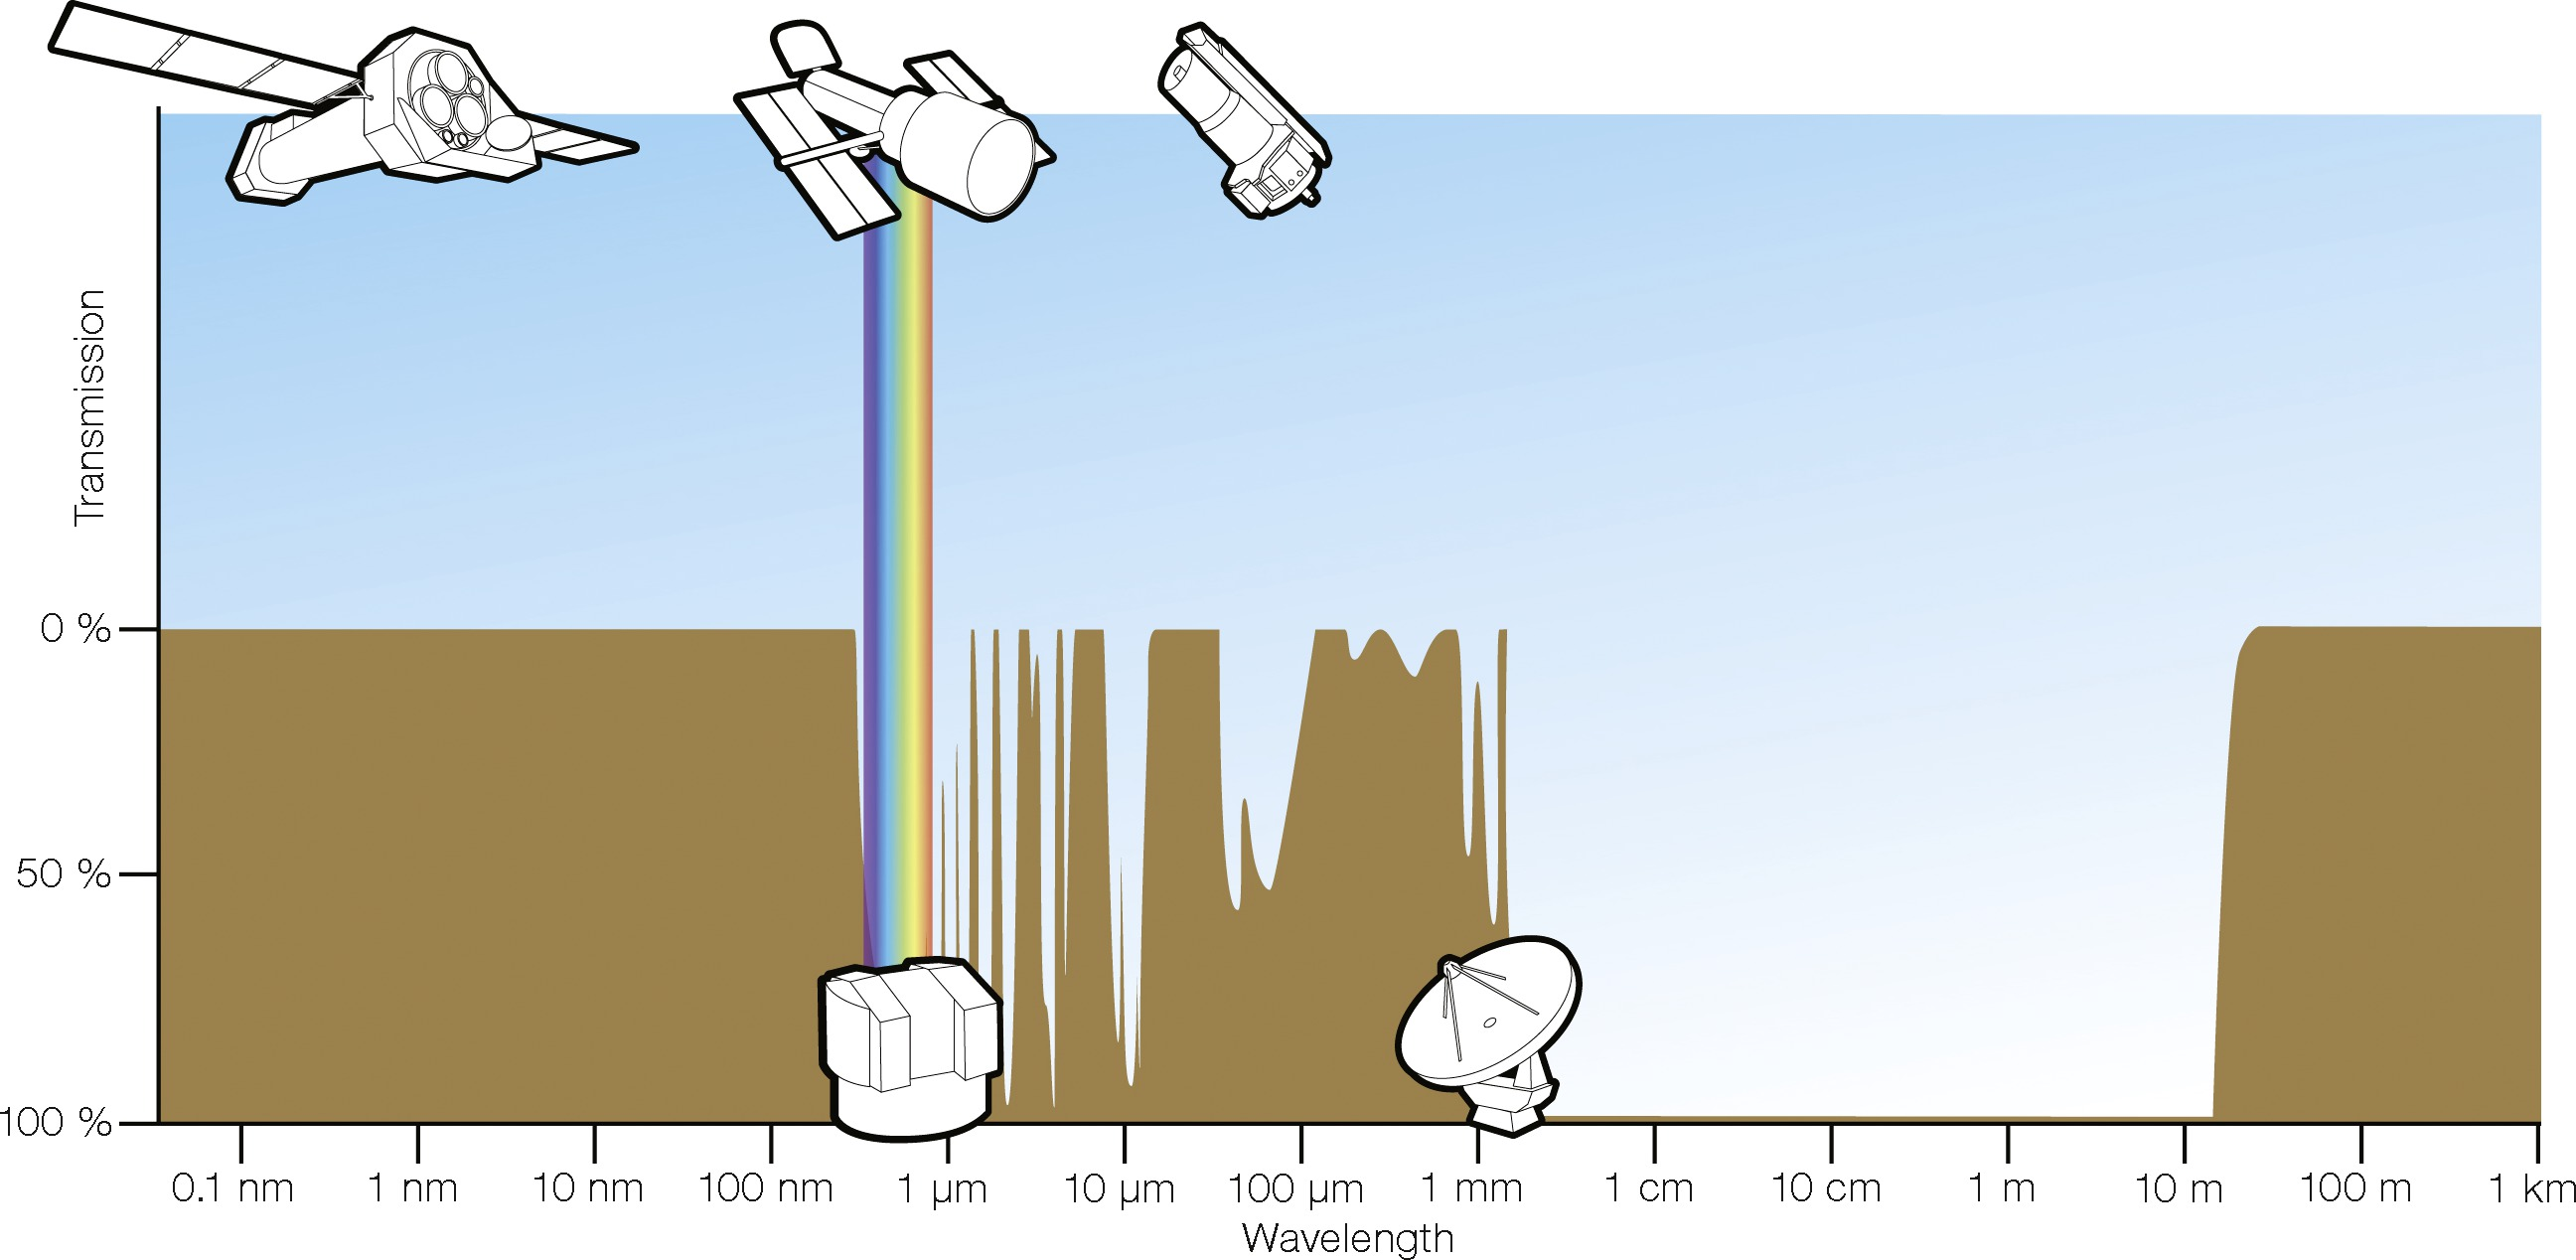
\includegraphics[width=\textwidth]{atmospheric-em-transmittance}
  \bicaption[大气层的电磁辐射透射率随波长的变化]{%
    大气层的电磁辐射\acs*{transmittance}随波长 $\lambda$(即频率 $\nu$)的变化。
    除了光学窗口,大气层还有一个更宽的射电窗口,
    从 $\lambda \sim \SI{0.3}{\mm}$ ($\nu \sim \SI{1000}{\GHz}$)
    延伸到 $\lambda \sim \SI{30}{\meter}$ ($\nu \sim \SI{10}{\MHz}$)。
  }{%
    Electromagnetic transmittance of the Earth's atmosphere.
    In addition to the visible optical window, there is another
    much wider radio window, which spans from
    $\lambda \sim \SI{0.3}{\mm}$ ($\nu \sim \SI{1000}{\GHz}$)
    to $\lambda \sim \SI{30}{\meter}$ ($\nu \sim \SI{10}{\MHz}$).
    \\来源/Credit:
    \citeay{condon2016}, \S\,1.1.2
  }
  \label{fig:atmospheric-emt}
\end{figure}

首次发现源自地球之外的射电辐射是在 1932 年被 Bell 电话实验室的工程师
Karl G. Jansky 意外得到的。
上世纪 20 年代,Bell 电话公司基于 $\lambda \sim \SI{15}{\meter}$
的短波传输建设了跨洋电话服务,但是发现通话受到了强烈的干扰,因此派 Jansky 去查明干扰来源。
Jansky 建造了一个对方向敏感的可转动天线(如\autoref{fig:jansky-antenna} 所示)
用来监测 \SI{20.5}{\MHz} ($\lambda \approx \SI{14.6}{\meter}$) 处的射电辐射。
经过观测,他发现绝大部分的干扰源自暴风雨的闪电。
但是除此之外,他还发现有一个较弱的不明噪声,其强度在每天发生周期性的变化。
因此 Jansky 怀疑该噪声可能是太阳的射电辐射。
但是持续的观测显示这个不明噪声的准确周期为 \SI{23}{\hour}\,\SI{56}{\minute},
并不是恰好 \SI{24}{\hour}。
将此困惑与他的一个天文学家朋友 Albert M. Skellett 讨论后,
Jansky 了解到该噪声来自太阳系之外,并进一步确认其来源是银河系中心 \cite{jansky1933}。

\begin{figure}[htp]
  \centering
  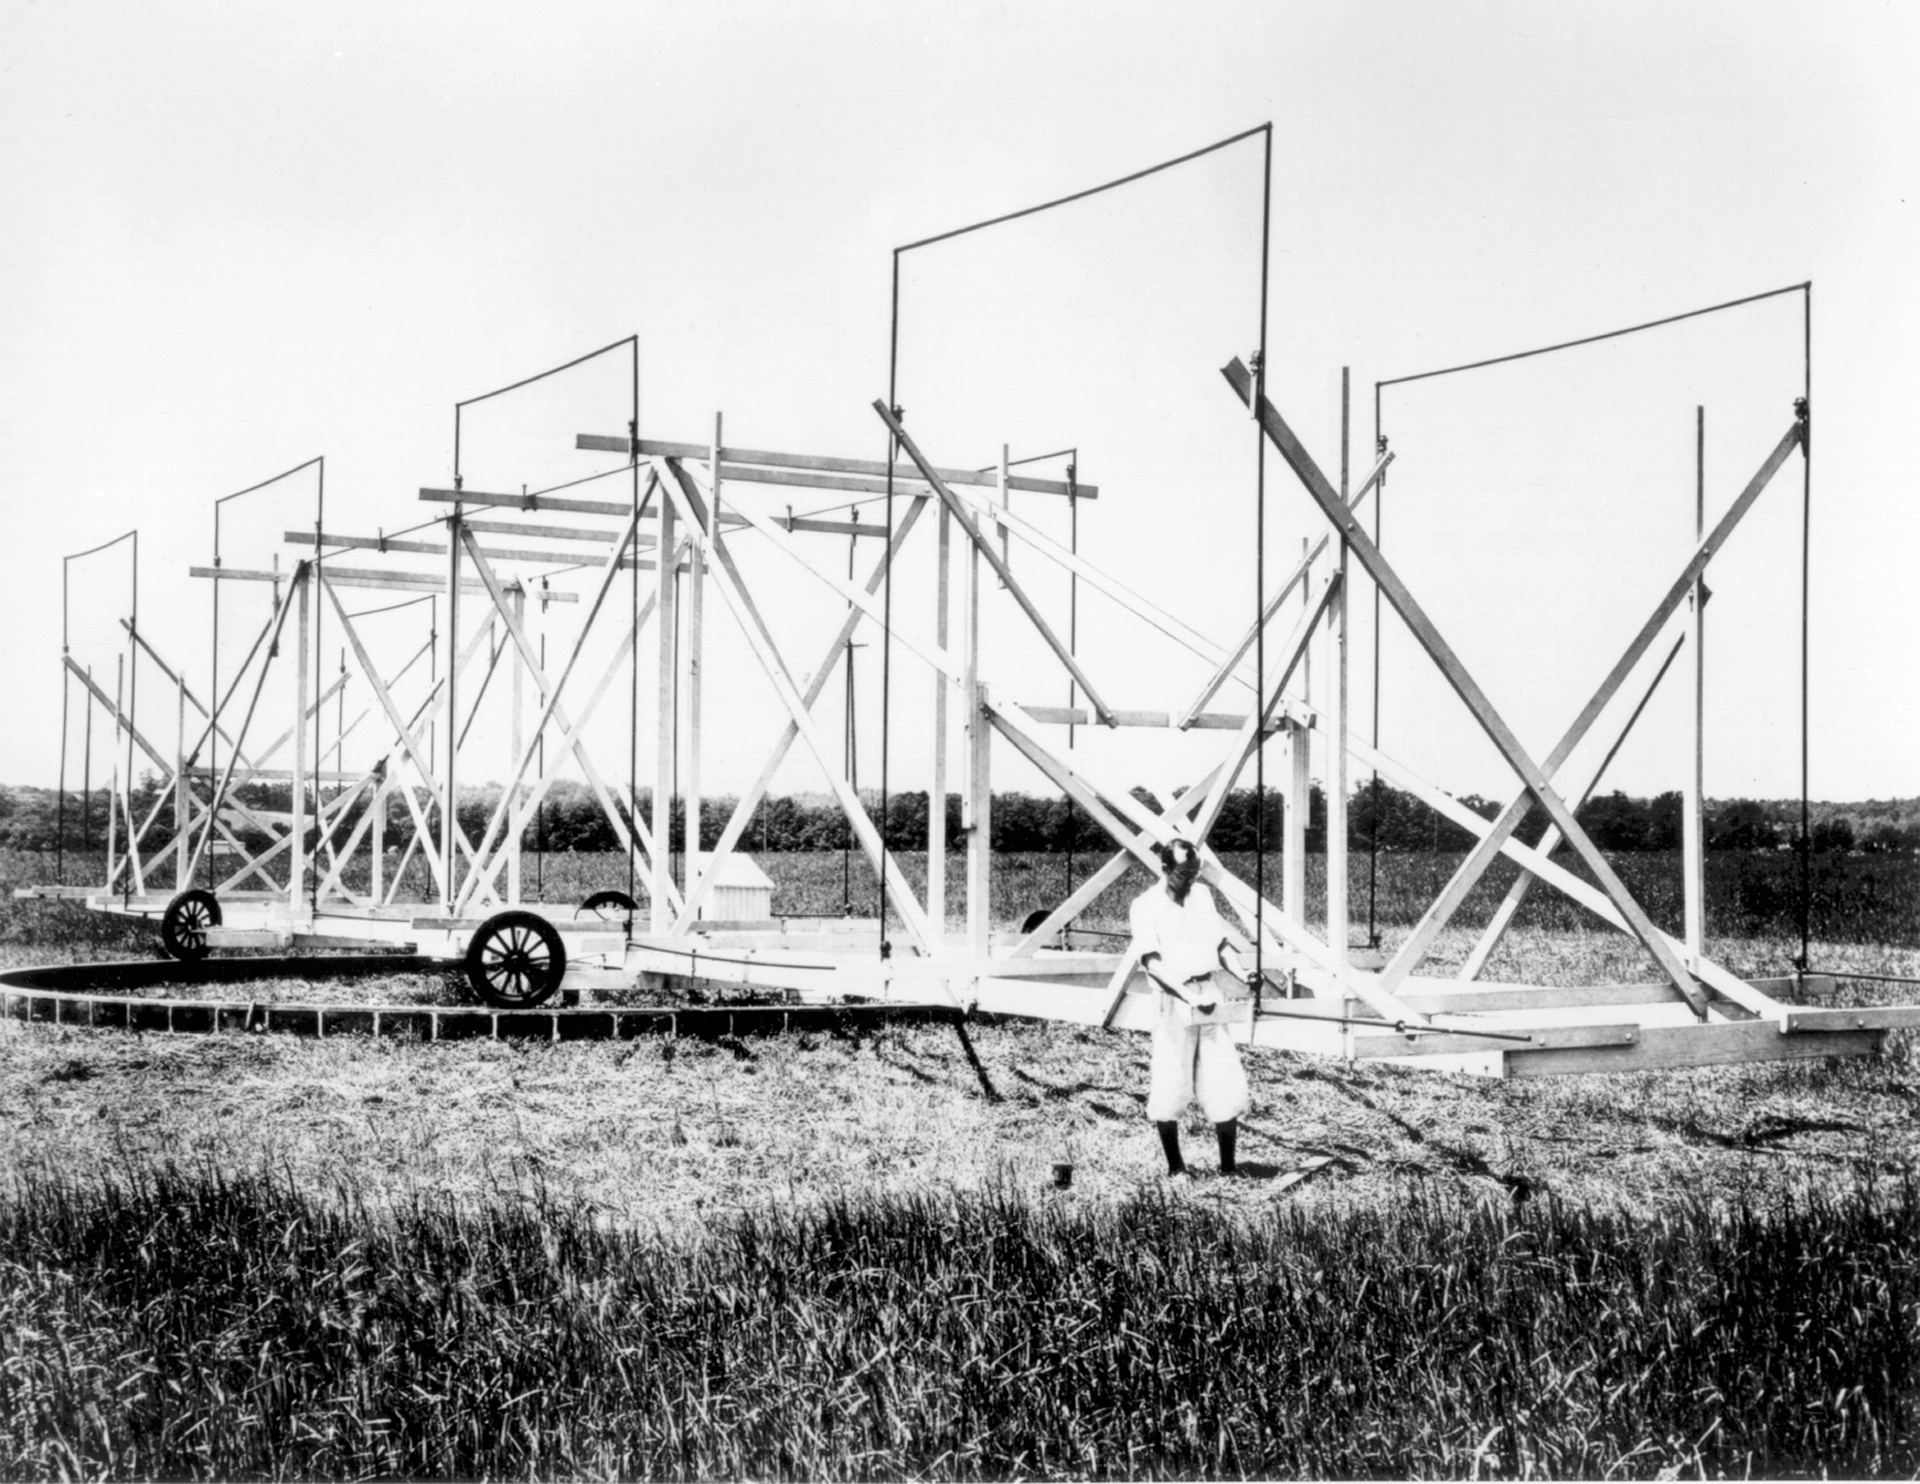
\includegraphics[width=0.8\textwidth]{KarlJansky-antenna}
  \bicaption[Karl G. Jansky 和他的天线]{%
    Karl G. Jansky 和帮助他发现银河系射电辐射的天线。
    该天线可转动,主要接收水平方向的辐射。
  }{%
    Karl G. Jansky and the antenna that discovered the
    Galactic radio emission.
    The antenna can rotate in azimuth and mainly receive horizontal
    emissions.
    \\来源/Credit:
    \ac{nrao}/\ac{aui}/\ac{nsf}
  }
  \label{fig:jansky-antenna}
\end{figure}

然而 Jansky 的发现未能得到足够的关注和重视,
他本人也被分配到其他项目而无法继续研究银河系的射电辐射。
另一位无线电工程师 Grote Reber 恰好对 Jansky 的发现产生了极大兴趣,
于是耗时数年在自家后院建造了世界第一台抛物面射电望远镜
(\autoref{fig:reber-telescope}),
并在 1938 年成功地在 \SI{160}{\MHz} 探测到了银河系的射电辐射。
Reber 接着进一步开展了银河系的第一次射电巡天观测,并将结果发表于专业的天文学期刊
\textit{The Astrophysical Journal} \cite{reber1940}。
自此,射电天文学登上了天文学的舞台。

\begin{figure}[htp]
  \centering
  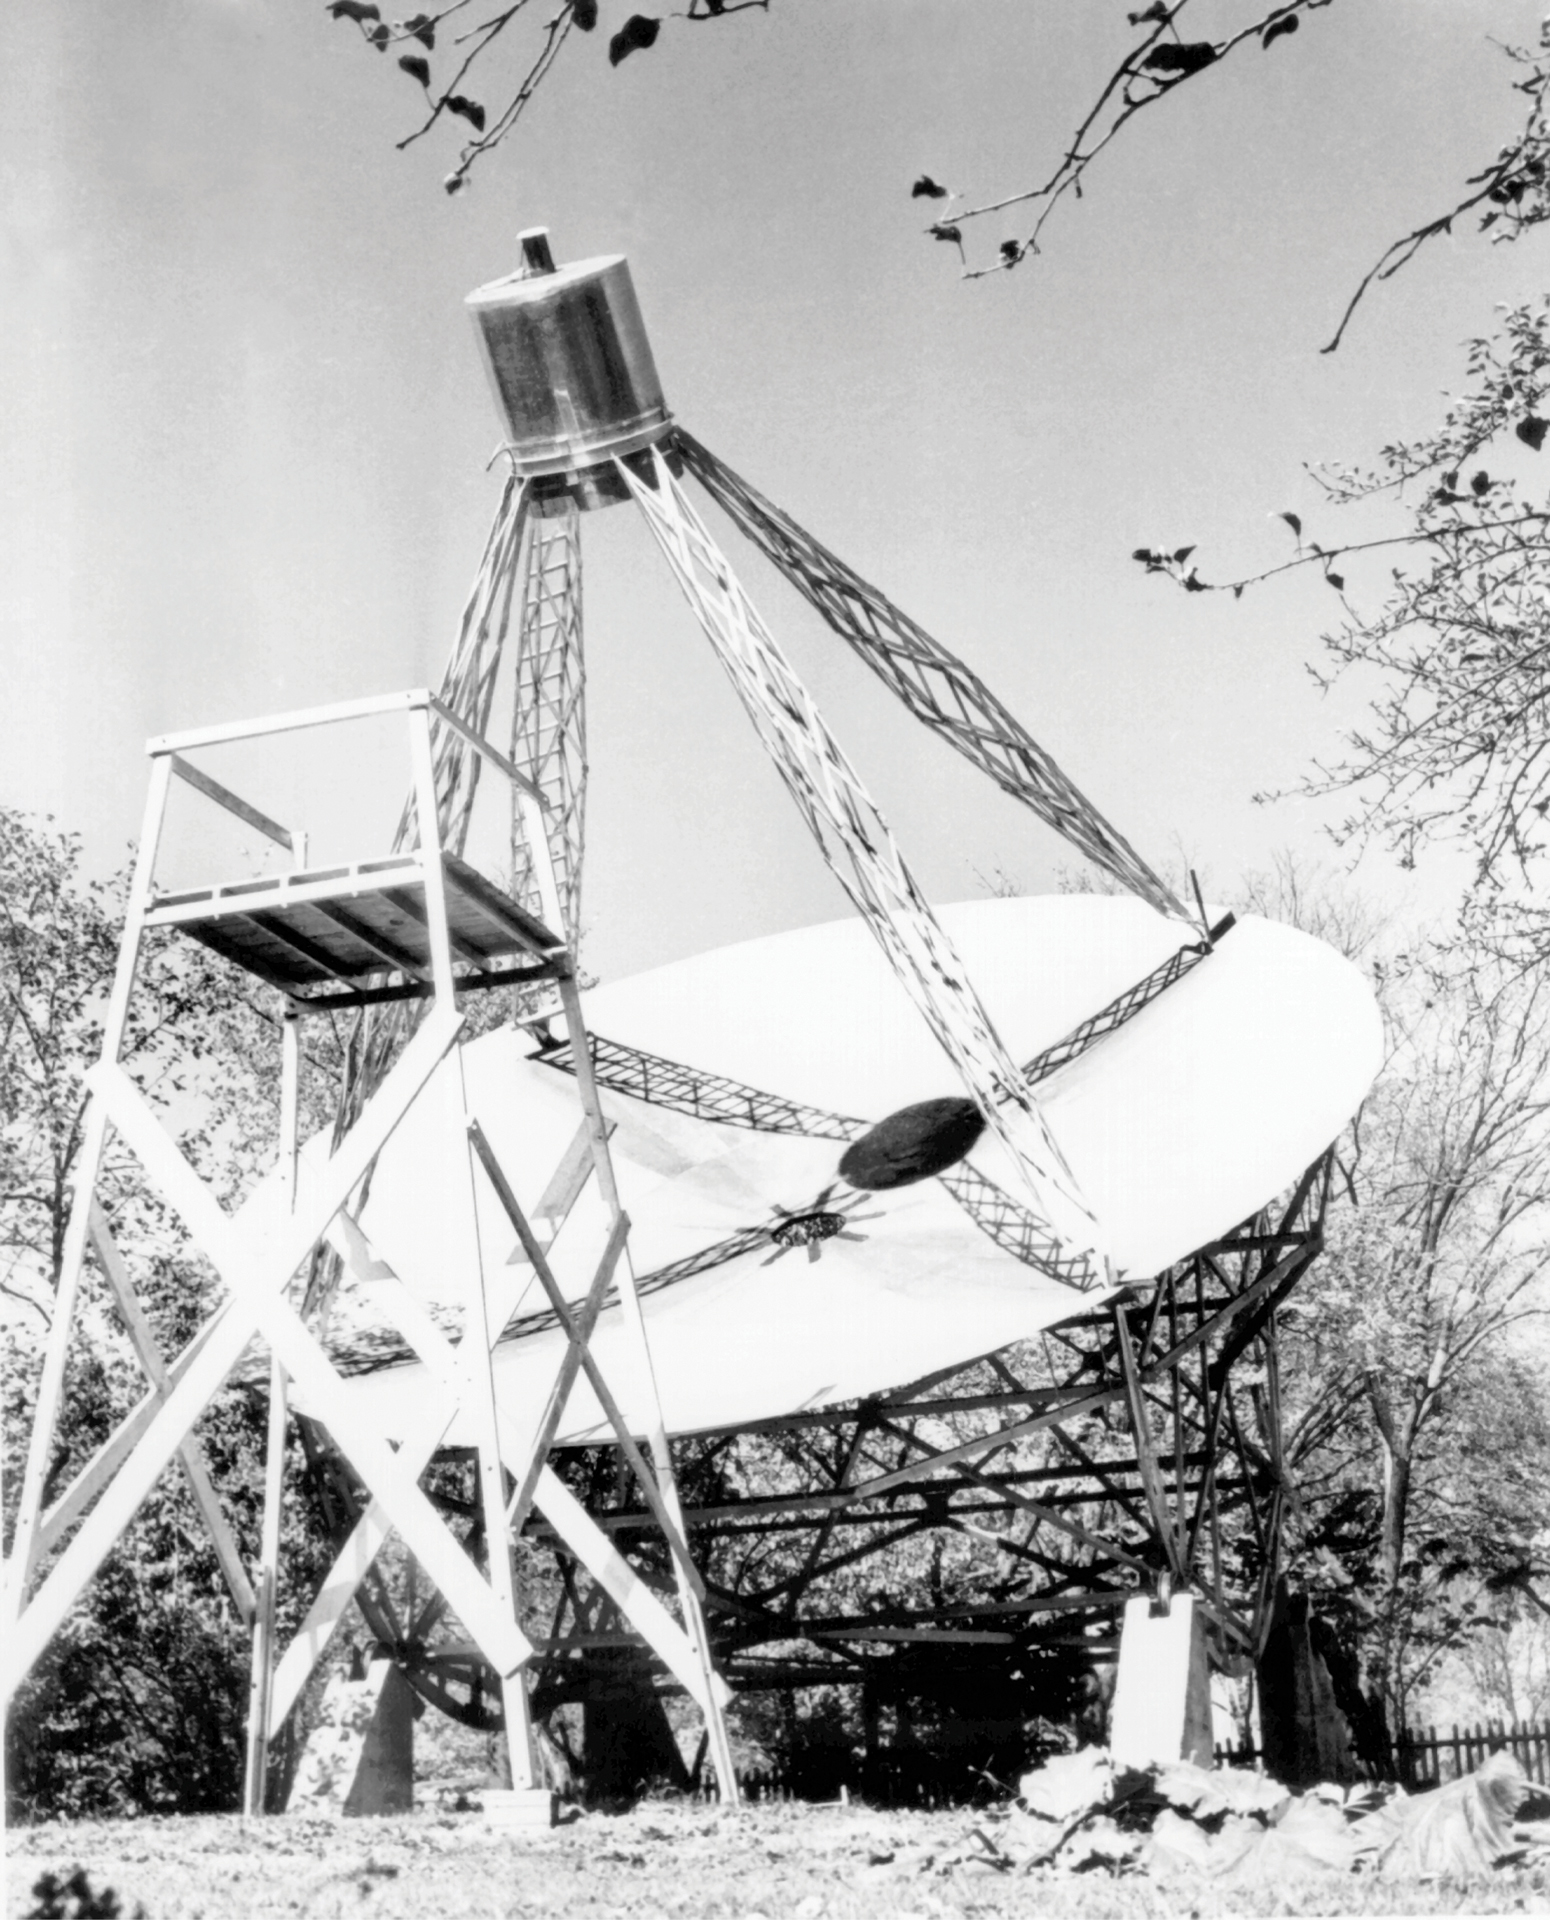
\includegraphics[width=0.6\textwidth]{GroteReber-telescope}
  \bicaption[Grote Reber 建造的抛物面射电望远镜]{%
    Grote Reber 在自家后院建造的射电望远镜,使用了直径约 \SI{10}{\meter} 的抛物面。
  }{%
    Grote Reber's backyard radio telescope using a parabolic reflector
    of diameter about \SI{10}{\meter}.
    \\来源/Credit:
    \acs{nrao}/\acs{aui}/\acs{nsf}
  }
  \label{fig:reber-telescope}
\end{figure}

在后续的几年里,尽管第二次世界大战阻碍了射电天文学的发展,
但是刺激了无线电技术和雷达设备的研发。
这些方面的成果在战争结束后给射电天文学带去了长足的进步,开创了一系列新技术和新方法。
其中最值得一提的是由 Martin Ryle 和 Antony Hewish 发明的\ac{as}技术 \cite{ryle1960},
使射电观测的角分辨率得到了空前的提高。

自射电窗口被打开以来,射电天文学已取得了一系列激动人心的发现,
其中代表性的发现包括:
银河系和其他多种天体的非热 (non-thermal) 辐射 \cite{reber1940}、
由超大质量黑洞驱动的射电星系\cite{baade1954}
和\ac{quasar}\cite{hazard1963,schmidt1963}、
冷\ac{ism}的热辐射谱线、
星际分子的\ac{maser} \cite{weaver1965}、
宇宙大爆炸的 \ac{cmb} \cite{penzias1965}、
\ac{pulsar}和中子星 \cite{hewish1968}、
星系中的\ac{dm} \cite{roberts1975}、
\ac{gl-strong} \cite{walsh1979}。
总之,射电天文学揭开了宇宙的全新一面(如\autoref{fig:radio-sky} 所示),
拓展了我们对宇宙的认识,深刻地改变了我们对宇宙的理解。

\begin{figure}[htp]
  \centering
  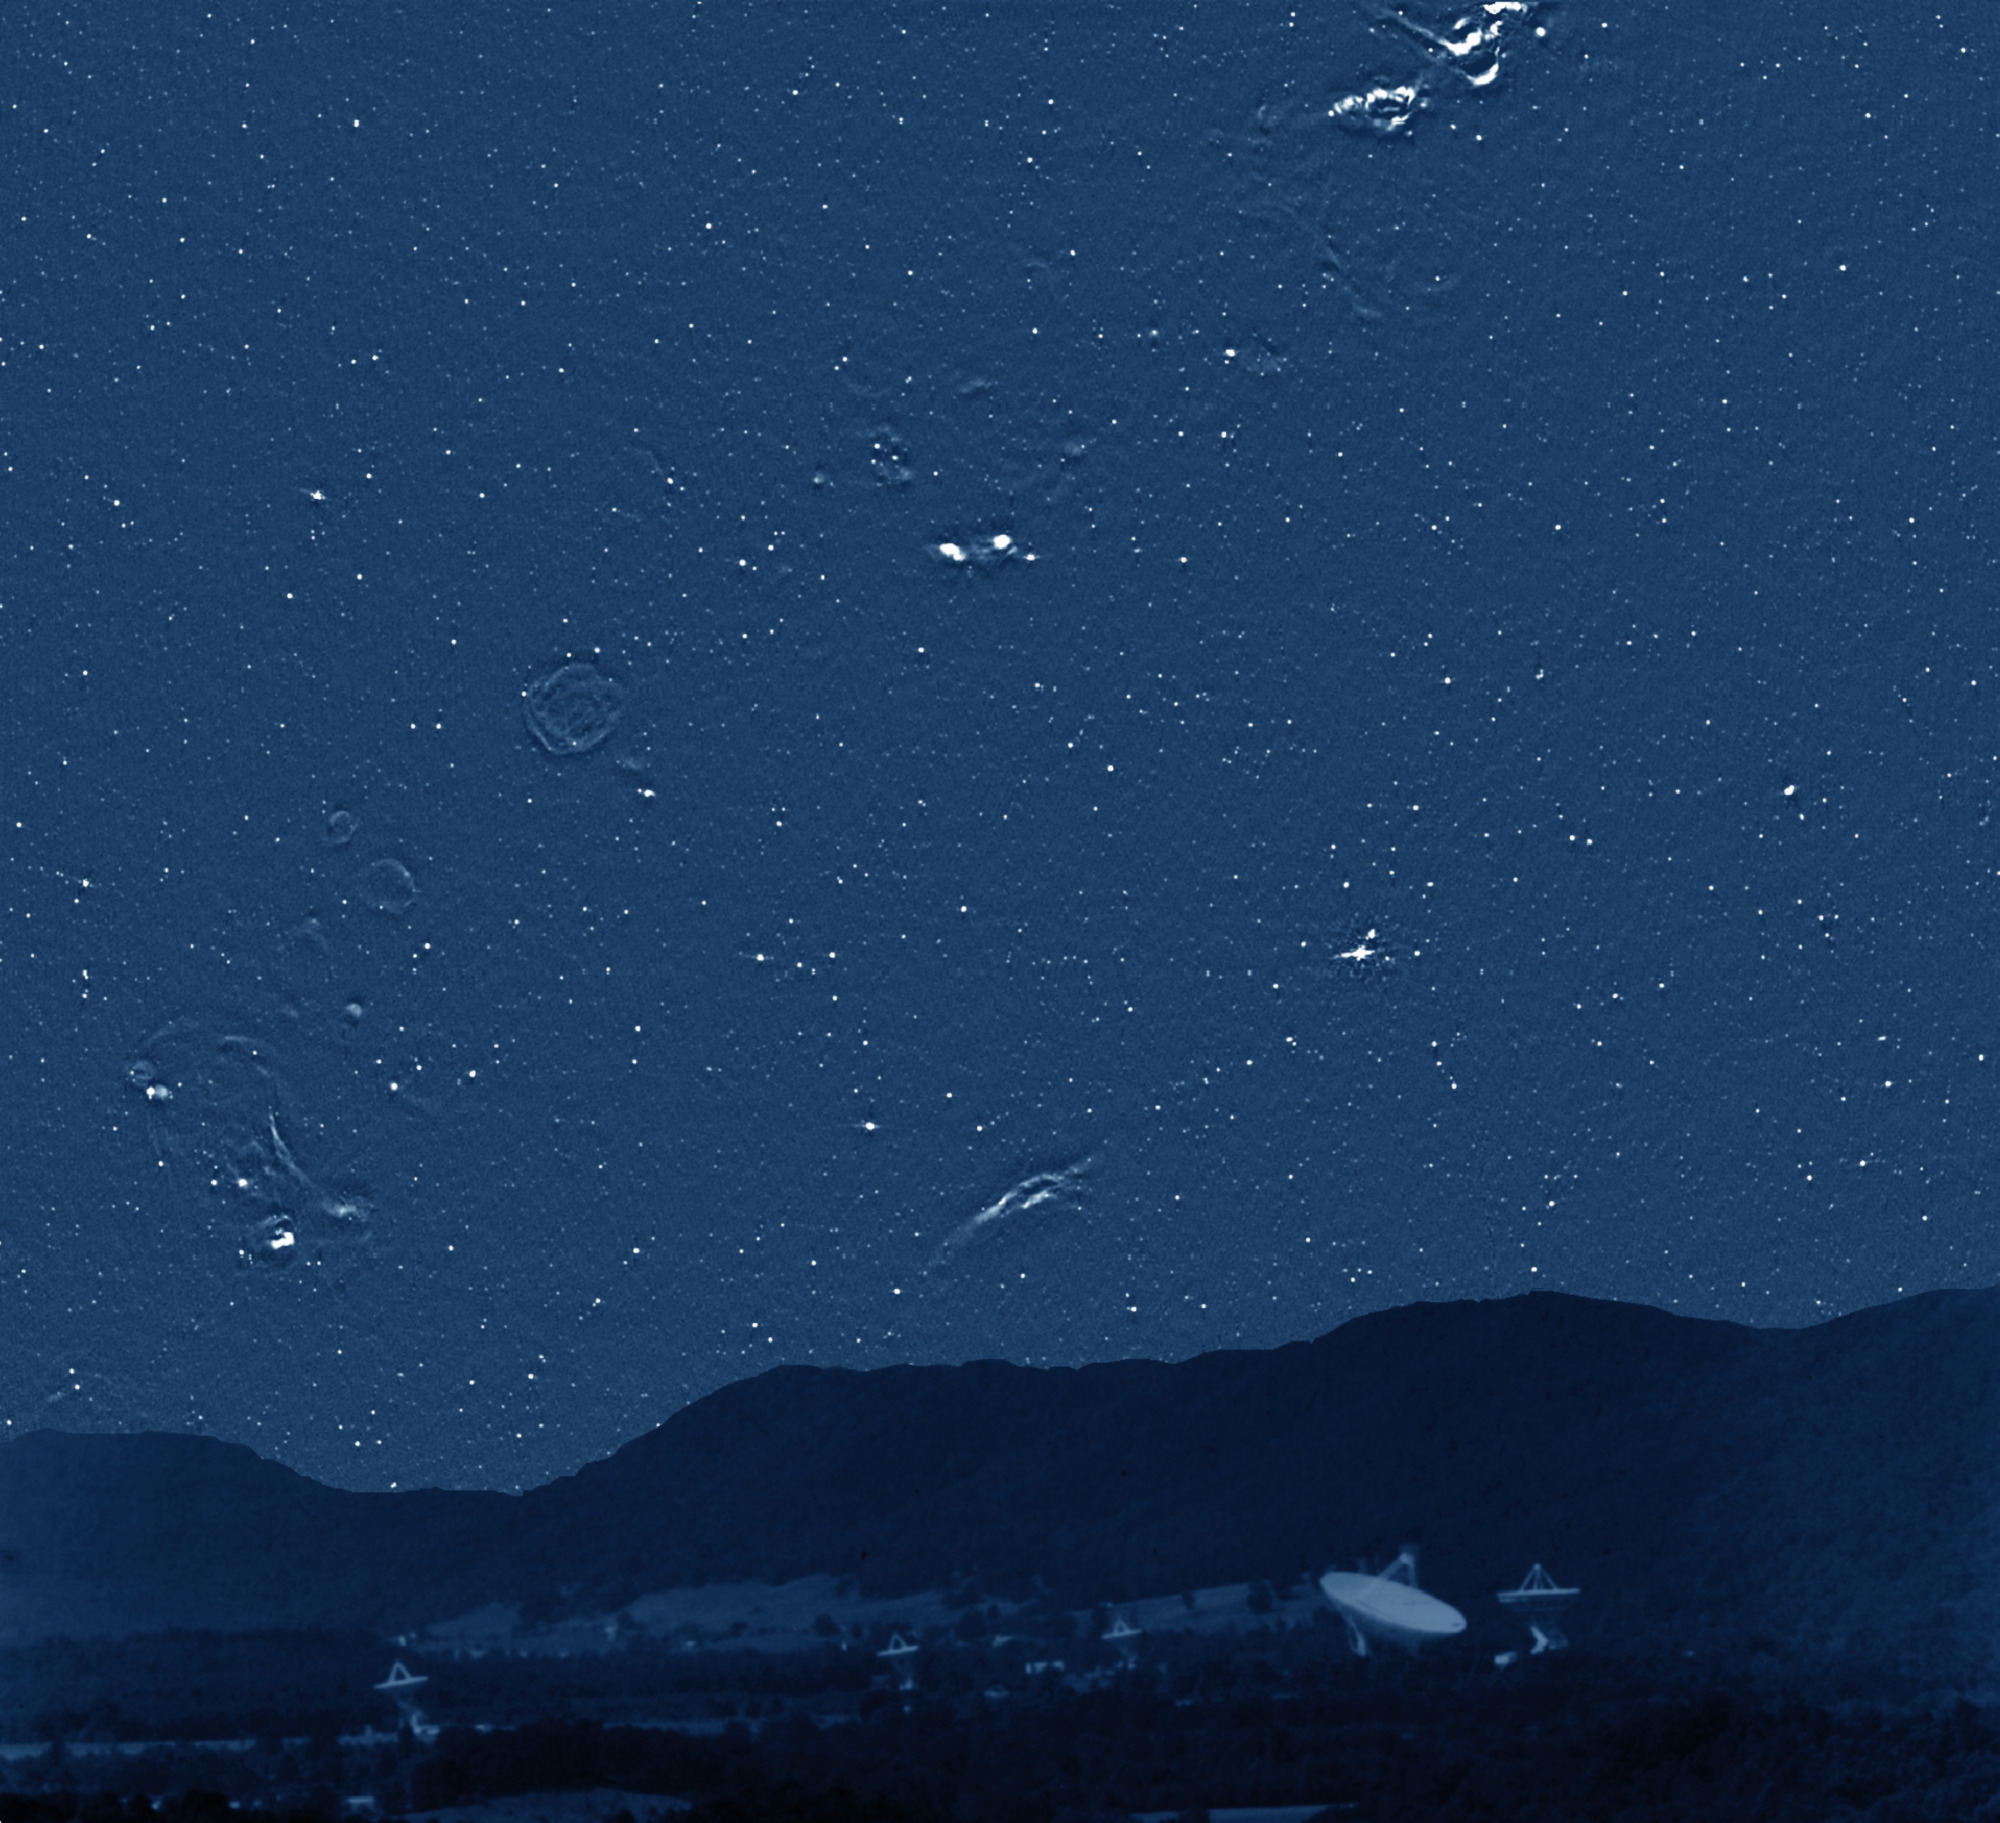
\includegraphics[width=0.8\textwidth]{nrao-radio-sky}
  \bicaption[与光学波段所见完全不同的射电天空]{%
    在 NRAO 台址的照片上方显示了由 NRAO 昔日的 \SI{91}{\meter} 射电望远镜
    获得的 \SI{4.85}{\GHz} 射电天空图像,展示了与光学波段所见完全不同的景象。
  }{%
    The \SI{4.85}{\GHz} radio sky made with the NRAO former \SI{91}{\meter}
    telescope is shown above an old photograph of the NRAO site,
    showing a very different scene from seeing in the optical band.
    \\来源/Credit:
    \acs{nrao}/\acs{aui}/\acs{nsf}
  }
  \label{fig:radio-sky}
\end{figure}

%---------------------------------------------------------------------
\subsection{低频波段的机遇和挑战}

尽管大气层的射电窗口允许低至 $\sim$\,\SI{10}{\MHz} 的观测,但由于各种技术和条件的限制,
以往的射电观测和研究主要在 $\gtrsim$\,\SI{1}{\GHz} 的中高频波段。
相比中高频波段,低频波段主要拥有以下几个优势:
\begin{itemize}
  \item 源自 EoR 的\ac{hi} \ac{21cmline}是目前研究该时期的最直接而有效的探针
    \cite{morales2010}。
    EoR 信号经过显著红移后将出现在 $\sim$\,\SIrange{90}{200}{\MHz}
    的低频射电波段,因此在此波段开展 EoR 信号探测实验具有重要意义
    \cite{mellema2013,mellema2015,koopmans2015}
    (详见 \autoref{sec:eor-signal})。
  \item 低频波段对应的辐射波长更长,受尘埃的影响更小,所以能够观测到星系更核心的区域。
  \item \ac{rad-syn}在低频波段更明亮而且寿命更长,因此更利于探测\ac{gc}、
    \ac{sc}甚至\ac{lsf}的弥散射电辐射 \cite{cassano2015,vazza2015,kale2016}。
  \item 多种等离子体效应(如散射、色散、Faraday 旋转)的强度按 $\nu^{-2}$ 变化,
    因此在低频波段更适合研究星际电子密度、磁场分布、等等
    \cite{johnston2015,roy2016,vanEck2017}。
  \item 低频射电望远镜通常具有大视场,能够显著提高巡天速度,
    便于搜寻脉冲星、暂现源、等等 \cite{stappers2011,fender2015}。
\end{itemize}

近十多年来,与低频射电相关的工程技术已取得长足的进步。
在射电天文学领域,低频射电波段也得到了重点关注,
目前已建成一批工作在此波段的干涉阵列,
主要包括 \ac{21cma}、\ac{gmrt}、\ac{mwa}、\ac{lofar}。
此外还有若干正在积极建设的新型低频干涉阵列,比如 \ac{lwa}、\ac{hera}、\ac{ska}。
可见,低频射电波段正在成为射电天文乃至整个天文领域的热点和前沿。

另一方面,在低频波段开展观测也面临更大的挑战。
为了实现较高的空间分辨率和灵敏度,通常需要建设较大规模的低频射电干涉阵列,
因此需要解决更复杂的仪器效应校准、研发更有效的数据处理方法。
此外,低频射电观测还需要应对更明亮的前景(如银河系的弥散辐射)干扰、
更强烈的人工源 \ac{rfi}、更剧烈的电离层扰动、等等
(参见 \autoref{sec:det-difficulties})。
尽管如此,可以肯定低频射电天文将成为射电天文领域的重要力量,
并为整个天文学的发展作出贡献。


%=====================================================================
\section{辐射理论基础}
\label{sec:radiation}

%---------------------------------------------------------------------
\subsection{\acl*{I-nu}、\acl*{S-nu}和\acl*{u-nu}}

\begin{figure}[htp]
  \centering
  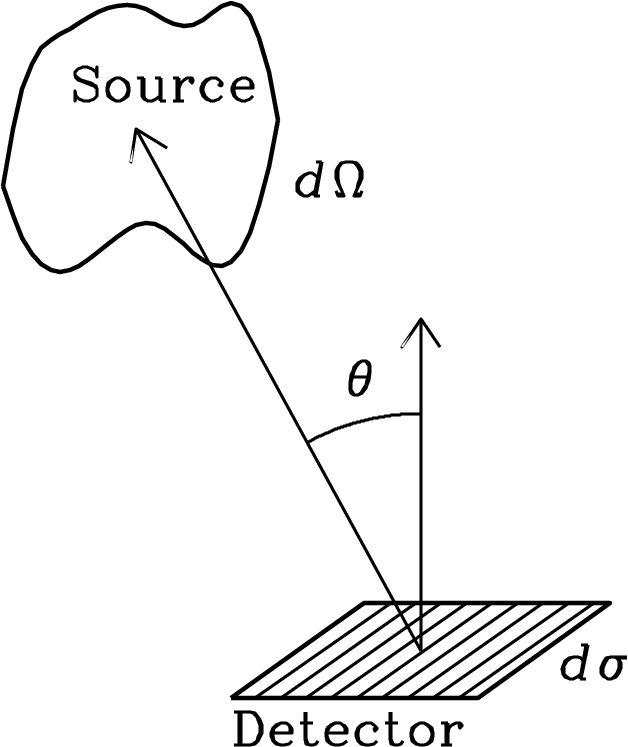
\includegraphics[width=0.3\textwidth]{specific-intensity}
  \bicaption{%
    \acl*{I-nu} \acs*{I-nu} 的测量示意图
  }{%
    The specific intensity \acs*{I-nu} measured by a detector of area
    $\D{\sigma}$ to a source extending a solid angle of $\D{\Omega}$.
    \\来源/Credit:
    \citeay{condon2016}, \S\,2.1
  }
  \label{fig:intensity}
\end{figure}

考虑一个面积为 $\D{\sigma}$ 的探测器,测量一个与其法线方向呈 $\theta$ 角度、
所张立体角为 $\D{\Omega}$ 的辐射源,如\autoref{fig:intensity} 所示。
若探测器在频率范围 $[\nu, \,\nu+\D{\nu}]$ 内接收到的功率为 $\D{P_{\nu}}$,
则这个源的\acl{I-nu} (specific intensity) \ac{I-nu} 定义为:
\begin{equation}
  \label{eq:intensity}
  \ac{I-nu} \equiv
    \frac{\D{P_{\nu}}}{(\cos\theta\,\D{\sigma}) \,\D{\nu} \,\D{\Omega}} \,,
\end{equation}
其 \ac{si} 单位是 [\si{\watt\per\square\meter\per\hertz\per\steradian}]。
\acl{I-nu} \ac{I-nu} 亦被称为\ac{spec-brightness},
有时也被简称为强度或亮度。

\begin{figure}[htp]
  \centering
  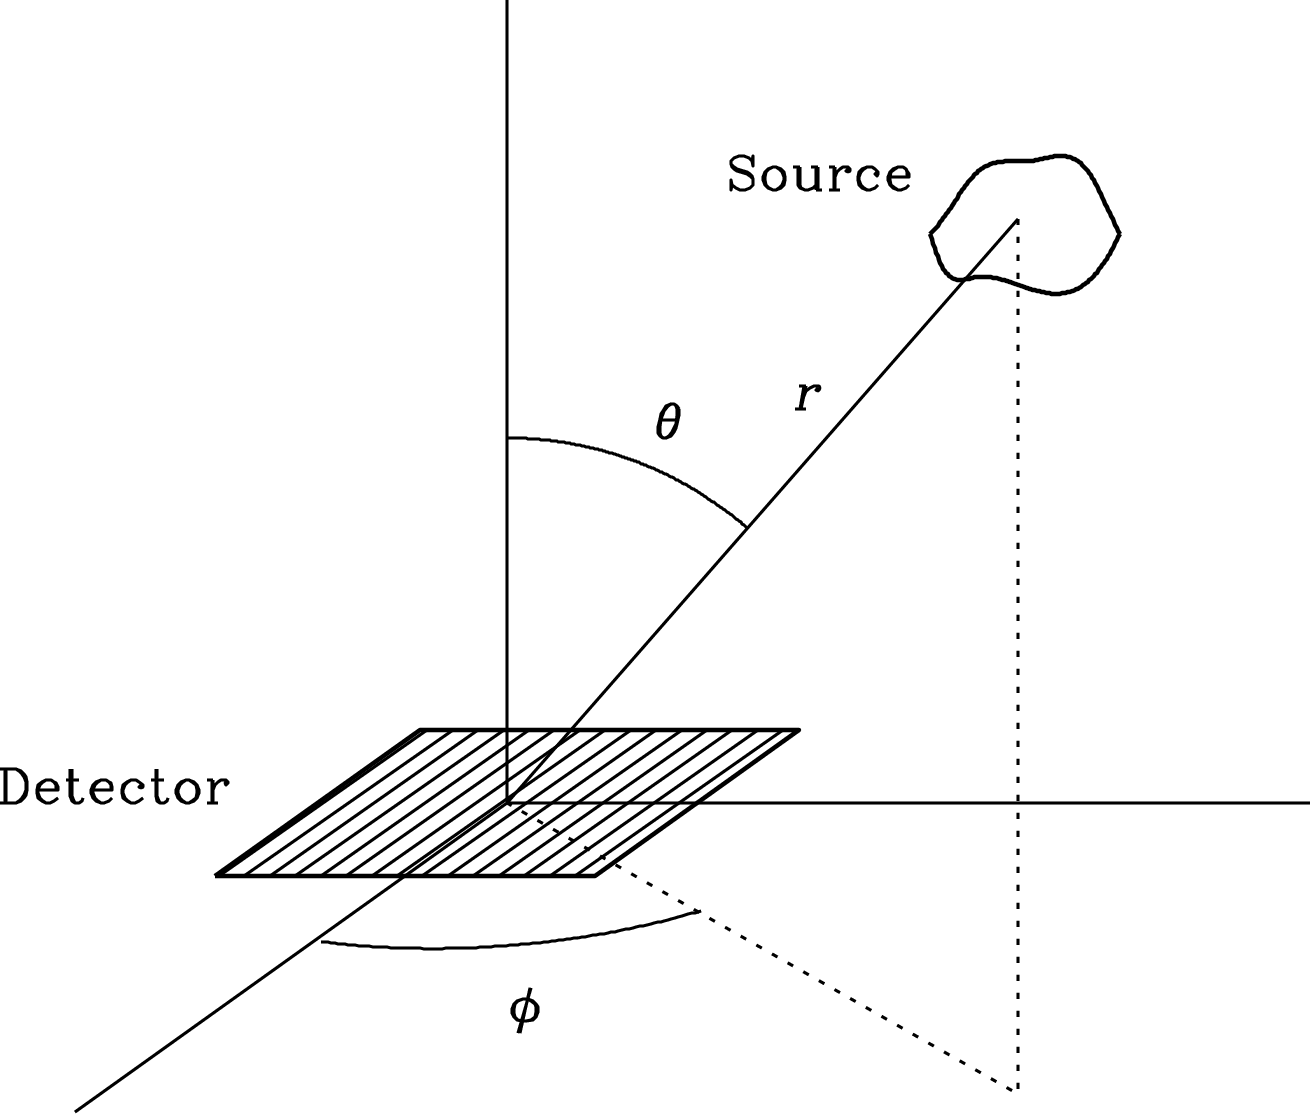
\includegraphics[width=0.6\textwidth]{flux-density}
  \bicaption{%
    \acl*{S-nu} \acs*{S-nu} 的定义示意图
  }{%
    An illustration of the definition of flux density \acs*{S-nu}.
    \\来源/Credit:
    \citeay{condon2016}, \S\,2.1
  }
  \label{fig:flux-density}
\end{figure}

一个\ac{src-discrete}所张的立体角是确定的(如\autoref{fig:flux-density} 所示),
因此探测器单位投影面积上接收到的\ac{spec-power}即为
这个源的\acl{S-nu} (flux density) \ac{S-nu}:
\begin{equation}
  \label{eq:flux-density}
  \ac{S-nu} \equiv
    \int_{\R{source}} \ac{I-nu}(\theta,\phi) \cos\theta \,\D{\Omega} ,
\end{equation}
其 \ac{si} 单位是 [\si{\watt\per\square\meter\per\hertz}]。
实际中常用单位 [\si{\jansky}],换算关系为
$\SI{1}{\jansky} = \SI{e-26}{\watt\per\square\meter\per\hertz}$。

一个辐射场的\acl{u-nu} (spectral energy density) 是指
每单位体积的\ac{spec-energy},具有 \ac{si} 单位
[\si{\joule\per\cubic\meter\per\hertz}]。
取辐射场中的一个体积元 $\D{V}$,
对于一束大小为 $\D{\Omega}$ 的辐射 $\ac{I-nu}(\theta,\phi)$,
可认为该体积元 $\D{V}$ 具有长度 $\D{s}$ 以及横截面积 $\D{\sigma}$,
即 $\D{V} = \D{s}\,\D{\sigma}$,
于是这束辐射 $\acs{I-nu}(\theta,\phi)$ 贡献给这个体积元的谱能量为:
\begin{equation}
  \D{\acs{u-nu}}\,\D{V}
    = \acs{I-nu}(\theta,\phi) \,\D{\Omega}\,\D{\sigma}
      \left( \frac{\D{s}}{\acs{speed-light}} \right) ,
\end{equation}
其中 \acs{speed-light} 是\acl{speed-light}。
所以源自 $\D{\Omega}$ 方向的辐射 $\acs{I-nu}(\theta,\phi)$
在体积元 $\D{V}$ 的位置贡献的\acl{u-nu}为:
\begin{equation}
  \D{\acs{u-nu}}
    = \frac{\acs{I-nu}(\theta,\phi)}{\acs{speed-light}} \,\D{\Omega} ,
\end{equation}
将上式对所有方向积分,即得辐射场的\acl{u-nu}:
\begin{equation}
  \label{eq:spectral-energy-density}
  \acs{u-nu}
    = \int_{4\Cpi} \D{\acs{u-nu}}
    = \frac{1}{\acs{speed-light}}
      \int_{4\Cpi} \acs{I-nu}(\theta,\phi) \,\D{\Omega} .
\end{equation}
如果辐射场是各向同性的,即 $\acs{I-nu}(\theta,\phi) = \acs{I-nu}$,则有:
\begin{equation}
  \label{eq:spectral-energy-density-iso}
  \acs{u-nu} = \frac{4\Cpi \, \acs{I-nu}}{\acs{speed-light}} .
\end{equation}

%---------------------------------------------------------------------
\subsection{辐射转移方程和光深}
\label{sec:radiative-transfer}

\begin{figure}[htp]
  \centering
  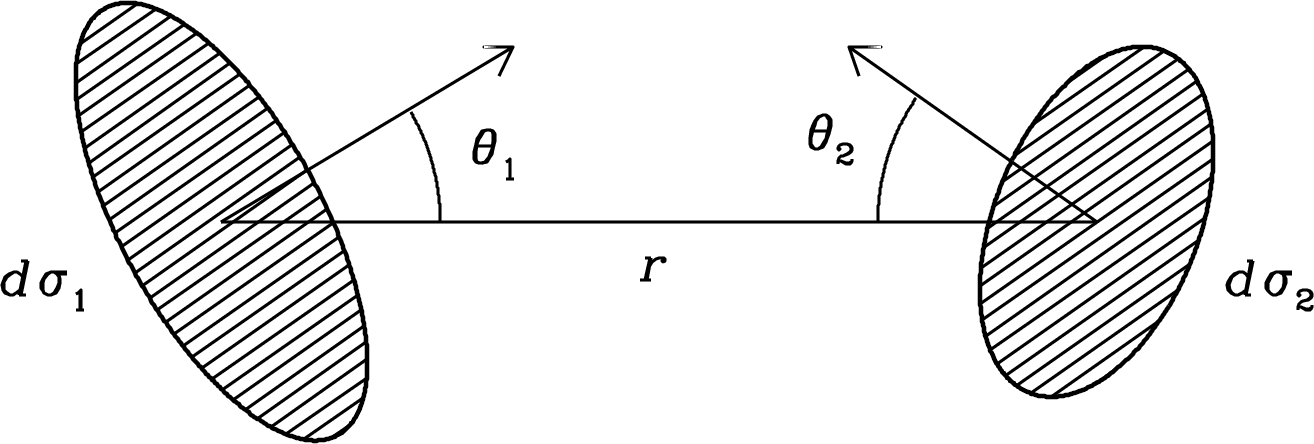
\includegraphics[width=0.6\textwidth]{specific-intensity-conservation}
  \bicaption{%
    \acl*{I-nu} \acs*{I-nu} 在自由空间里沿光线保持不变
  }{%
    The specific intensity \acs*{I-nu} conserved along a ray in empty space.
    \\来源/Credit:
    \citeay{condon2016}, \S\,2.1
  }
  \label{fig:intensity-conservation}
\end{figure}

辐射在不存在吸收和发射的自由空间里传播时,其强度保持不变,
即辐射的\acl*{I-nu} \acs*{I-nu} 与传播距离无关。
为了说明这一点,考虑由源发射的一束光线,
设 $\D{\sigma_1}$ 和 $\D{\sigma_2}$ 是光线上相距为 $r$ 的两个面元
(如\autoref{fig:intensity-conservation} 所示),
则两个面元相互所张的立体角分别为:
\begin{align}
  \D{\Omega_1} & = \frac{\cos\theta_2 \,\D{\sigma_2}}{r^2} , \\
  \D{\Omega_2} & = \frac{\cos\theta_1 \,\D{\sigma_1}}{r^2} .
\end{align}
于是可知在频率范围 $[\nu, \,\nu+\D{\nu}]$ 以及立体角 $\D{\Omega_1}$ 之内
流过面元 $\D{\sigma_1}$ 的功率为:
\begin{align}
  \D{P_1} & = (\acs{I-nu})_1 \cos\theta_1
      \,\D{\Omega_1} \,\D{\sigma_1} \,\D{\nu}  \\
    & = (\acs{I-nu})_1 \left( \frac{\cos\theta_1 \cos\theta_2}{r^2} \right)
      \,\D{\sigma_1} \,\D{\sigma_2} \,\D{\nu} ,
\end{align}
类似地,流过面元 $\D{\sigma_2}$ 的功率为:
\begin{align}
  \D{P_2} & = (\acs{I-nu})_2 \cos\theta_2
      \,\D{\Omega_2} \,\D{\sigma_2} \,\D{\nu}  \\
    & = (\acs{I-nu})_2 \left( \frac{\cos\theta_1 \cos\theta_2}{r^2} \right)
      \,\D{\sigma_1} \,\D{\sigma_2} \,\D{\nu} .
\end{align}
根据能量守恒,即 $\D{P_1}\,\D{t} = \D{P_2}\,\D{t}$,
可得:
\begin{equation}
  \label{eq:intensity-conservation}
  (\acs{I-nu})_1 = (\acs{I-nu})_2 .
\end{equation}

\begin{figure}[htp]
  \centering
  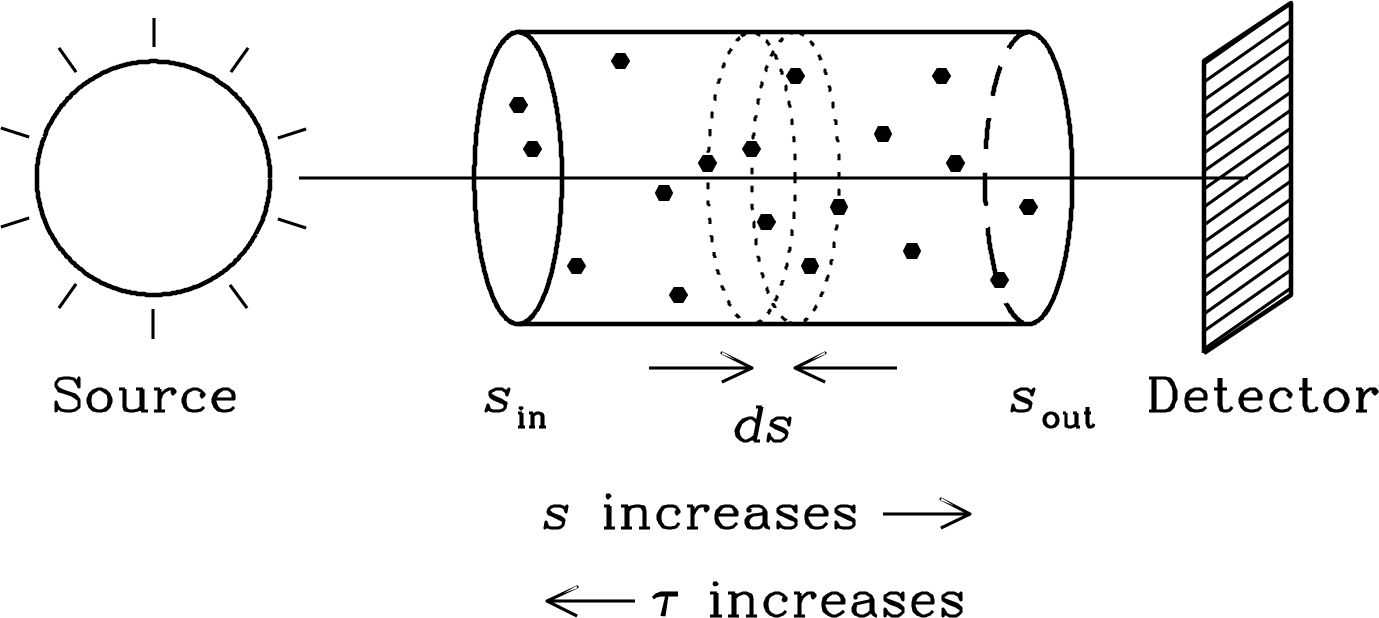
\includegraphics[width=0.6\textwidth]{radiative-transfer}
  \bicaption[辐射转移示意图]{%
    辐射转移示意图。
    距离 $s$ 沿源向探测器的方向增长,介质的入射端和出射端的距离分别为
    $s_{\R{in}}$ 和 $s_{\R{out}}$。
    光深 $\tau$ 的增长方向与 $s$ 相反。
  }{%
    An illustration of the radiative transfer.
    The distance $s$ increases along the ray from the source to the detector.
    The distances at the input end and the output end of the intervening
    medium are $s_{\R{in}}$ and $s_{\R{out}}$, respectively.
    The optical depth $\tau$ is measured in the opposite direction as $s$.
    \\来源/Credit:
    \citeay{condon2016}, \S\,2.2
  }
  \label{fig:radiative-transfer}
\end{figure}

当传播空间中存在吸收和发射时(如\autoref{fig:radiative-transfer} 所示),
辐射的\acl{I-nu} \acs{I-nu} 会发生改变,具体变化可由\acf{rt}方程描述。
首先考虑吸收情形,一个辐射光子通过介质中一个厚度为 $\D{s}$ 的薄层时被吸收的概率 $\D{p}$ 为:
\begin{equation}
  \D{p} = \acs{coef-absorption} \,\D{s} ,
\end{equation}
其中 \acs{coef-absorption}
为\acl{coef-absorption} (absorption coefficient),
具有 \ac{si} 单位 [\si{\per\meter}]。
于是\acl{I-nu} \acs{I-nu} 在通过厚度 $\D{s}$ 的介质后的损失比例为:
\begin{equation}
  \label{eq:rt-absorption}
  \frac{\D{\acs{I-nu}}}{\acs{I-nu}} = - \acs{coef-absorption} \,\D{s} .
\end{equation}
对上式的两边沿介质的吸收路径积分,可得:
\begin{equation}
  \int_{s_{\R{in}}}^{s_{\R{out}}} \frac{\D{\acs{I-nu}}}{\acs{I-nu}}
    = \ln\acs{I-nu} \,\Big|_{s_{\R{in}}}^{s_{\R{out}}}
    = - \int_{s_{\R{in}}}^{s_{\R{out}}} \acs{coef-absorption}(s') \,\D{s'} ,
\end{equation}
即
\begin{equation}
  \label{eq:intensity-loss1}
  \frac{\acs{I-nu}(s_{\R{out}})}{\acs{I-nu}(s_{\R{in}})} =
    \exp \left[ - \int_{s_{\R{in}}}^{s_{\R{out}}}
      \acs{coef-absorption}(s') \,\D{s'} \right] .
\end{equation}
据此,可定义\acl{optical-depth} (optical depth) 为:
\begin{equation}
  \label{eq:optical-depth}
  \acs{optical-depth} \equiv
    - \int_{s_{\R{out}}}^{s_{\R{in}}} \acs{coef-absorption}(s') \,\D{s'} .
\end{equation}
注意,上式的积分方向与 $s$ 相反(参见\autoref{fig:radiative-transfer}),
如此可使 $\tau > 0$ 并且与介质的观测深度成正相关。
利用\acl{optical-depth} \acs{optical-depth},
可将\autoref{eq:intensity-loss1} 写成:
\begin{equation}
  \label{eq:intensity-loss}
  \frac{\acs{I-nu}(s_{\R{out}})}{\acs{I-nu}(s_{\R{in}})} =
    \exp (-\acs{optical-depth}) .
\end{equation}
当 $\tau \ll 1$ 时,称介质是光学薄的;
当 $\tau \gg 1$ 时,则称介质是光学厚的。

另一方面,介质可能产生辐射而使\acl{I-nu} \acs{I-nu} 增大。
考虑介质中的一个体积元 $\D{s}\,\D{\sigma}$,在频率范围 $[\nu, \,\nu+\D{\nu}]$ 内
沿某一方向的立体角元 $\D{\Omega}$ 所发射的谱功率为:
\begin{equation}
  \D{P_{\nu}} =
    \acs{coef-emission} \,\D{s}\,\D{\sigma}\,\D{\nu}\,\D{\Omega} ,
\end{equation}
其中 \acs{coef-emission} 为\acl{coef-emission} (emission coefficient),
在不存在吸收的情况下可表示为:
\begin{equation}
  \label{eq:coef-emission}
  \acs{coef-emission} = \diff{\acs{I-nu}}{s} ,
\end{equation}
具有 \ac{si} 单位 [\si{\watt\per\cubic\meter\per\hertz\per\steradian}]。
综合上式和\autoref{eq:rt-absorption},可得完整的\ac{rt}方程为:
\begin{equation}
  \label{eq:radiative-transfer}
  \diff{\acs{I-nu}}{s} =
    - \acs{coef-absorption} \,\acs{I-nu} + \acs{coef-emission} .
\end{equation}

%---------------------------------------------------------------------
\subsection{热平衡和 Kirchhoff 定律}

\acf{te},简称热平衡,
是指一个系统在没有外界影响的条件下,其各部分的宏观属性在长时间内不发生任何变化的状态。
这是热力学的一个基本实验定律,是定义温度的基础。

\begin{figure}[htp]
  \centering
  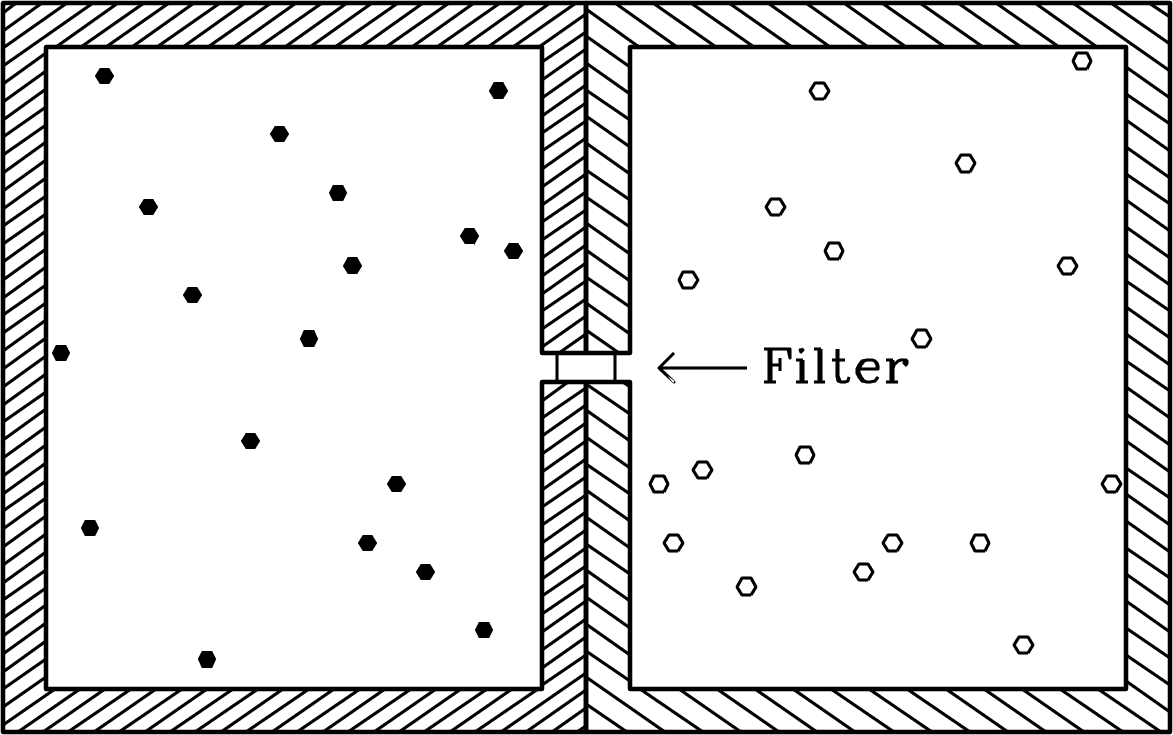
\includegraphics[width=0.5\textwidth]{Kirchhoff-law-experiment}
  \bicaption{%
    推导 Kirchhoff 定律的思想实验
  }{%
    A thought experiment to derive the Kirchhoff's law.
    \\来源/Credit:
    \citeay{condon2016}, \S\,2.2
  }
  \label{fig:kirchhoff-experiment}
\end{figure}

考虑如下思想实验:
两个由不同材料制成、包含不同介质的空腔放在一起,
中间由一个仅允许频率在 $[\nu, \,\nu+\D{\nu}]$ 之间的辐射通过的阀门连接,
如\autoref{fig:kirchhoff-experiment} 所示。
在完全热平衡的情形下,即空腔中的介质和辐射场具有相同的温度,
空腔产生的辐射与黑体辐射(详见后文 \autoref{sec:blackbody})相同,
完全由温度决定,而与其材质或者内部介质无关。
当两个空腔在任意温度 $T$ 达到完全热平衡时,
没有净能量从一个空腔通过阀门进入到另一个空腔,
否则损失能量的空腔将会冷却,另一个空腔将会升温,从而违背热力学第二定律。
由此可知:
\begin{align}
  \diff{\acs{I-nu}}{s} & = 0 , \\
  \acs{I-nu} & = B_{\nu}(T) ,
  \label{eq:kirchhoff-I-B}
\end{align}
其中 $B_{\nu}(T)$ 为空腔的辐射频谱。
于是辐射转移方程 [\autoref{eq:radiative-transfer}] 成为:
\begin{equation}
  \diff{\acs{I-nu}}{s} = 0
    = - \acs{coef-absorption} \,B_{\nu}(T) + \acs{coef-emission} ,
\end{equation}
所以:
\begin{equation}
  \label{eq:kirchhoff-law}
  \frac{\acs{coef-emission}(T)}{\acs{coef-absorption}(T)} = B_{\nu}(T) ,
\end{equation}
上式对任意频率 $\nu$ 均成立。
这就是完全热平衡系统的 Kirchhoff 定律。

完全热平衡状态只有在特殊的条件下才能实现;
对于一般的系统,介质无法与辐射场达到热平衡。
尽管如此,如果介质本身是热平衡的,则称该系统处于\acf{lte}状态。
对于这类\ac{lte}系统,Kirchhoff 定律 [\autoref{eq:kirchhoff-law}] 同样适用,
但是辐射场的\acl{I-nu} \ac{I-nu} 与介质的辐射频谱 $B_{\nu}(T)$ 通常不相等,
即\autoref{eq:kirchhoff-I-B} 不成立。

%---------------------------------------------------------------------
\subsection{黑体辐射和亮温度}
\label{sec:blackbody}

黑体是一个能够吸收全部入射辐射而不产生任何反射或透射的理想化物体。
处于热力学平衡态的黑体所发出的辐射称为黑体辐射,其能谱分布只取决于黑体的温度,
由 Planck 辐射定律给出:
\begin{equation}
  \label{eq:planck}
  B_{\nu}(\nu, T) = \frac{2 \acs{hp} \nu^3}{\acs{speed-light}^2}
    \left[ \exp\left( \frac{\acs{hp} \nu}{\acs{kb} T} \right) - 1 \right]^{-1} ,
\end{equation}
其中 $B_{\nu}$ 是谱亮度,
\acs{hp} 是 \acl{hp},
\acs{kb} 是 \acl{kb},
\acs{speed-light} 是\acl{speed-light}。

在射电波段,$\acs{hp}\nu \ll \acs{kb}T$ 通常成立,因此上式可近似为:
\begin{equation}
  \label{eq:rj-approx}
  B_{\nu}(\nu, T)
    \approx \frac{2 \nu^2 \acs{kb} T}{\acs{speed-light}^2} .
\end{equation}
这就是 Rayleigh--Jeans 近似。
在该近似下,黑体的谱亮度 $B_{\nu}$ 与其温度 $T$ 严格成正比。
因此,一个源的亮度(即\acl{I-nu}) \ac{I-nu}
可以很方便地使用\acl{T-b} (brightness temperature) \ac{T-b} 来描述:
\begin{equation}
  \label{eq:Tb}
  \acs{T-b}(\nu)
    \equiv \frac{\acs{I-nu} \acs{speed-light}^2}{2 \,\acs{kb} \nu^2} .
\end{equation}
对于一般的辐射源,其\acl{T-b} \ac{T-b} 会随频率 $\nu$ 发生改变。

%---------------------------------------------------------------------
\subsection{电阻的热噪声}

一个温度为 $T$ 的电阻 (resistor) 会因为内部电子的随机热运动而产生噪声,
称为 Johnson--Nyquist 噪声 \cite{johnson1928,nyquist1928},
其\ac{spec-power}由以下 Nyquist 近似给出
(详见 \citeay{condon2016}, \S\,2.5):
\begin{equation}
  \label{eq:nyquist-approx}
  P_{\nu} \approx \acs{kb} T .
\end{equation}
该式是 Rayleigh--Jeans 近似 [\autoref{eq:rj-approx}] 在电子学中的对应。
类似地,该近似公式只适用于 $\acs{hp}\nu \ll \acs{kb}T$ 的经典范畴。
在考虑量子化修正后,严格的 Nyquist 公式为:
\begin{equation}
  \label{eq:nyquist}
  P_{\nu} = \acs{hp} \nu
    \left[ \exp\left( \frac{\acs{hp} \nu}{\acs{kb} T} \right) - 1 \right]^{-1} .
\end{equation}


%=====================================================================
\section{谱线辐射基础}
\label{sec:spectral-line}

\acf{spec-line}是光谱上的窄($\Delta\nu \ll \nu$)发射或吸收特征,
源自原子或分子的能级跃迁。
当一个原子或分子从高能级 $E_2$ 跃迁至低能级 $E_1$ 时,会发射一个特定频率的光子,
一群这样的光子便形成了一条发射线 (emission line)。
反过来,如果一个原子或分子从低能级 $E_1$ 跃迁至高能级 $E_2$,
则会吸收一个特定频率的光子。
这些被吸收的光子通常来自背景的连续谱辐射,
因此观测到的连续谱上将出现一条吸收线 (absorption line)。
典型的谱线包括\ac{hii}的复合线、中性氢的 21\,cm 超精细结构谱线
(详见 \autoref{sec:21cm-line})。

%---------------------------------------------------------------------
\subsection{Einstein 系数和细致平衡方程}

\begin{figure}[htp]
  \centering
  \includegraphics[width=0.9\textwidth]{atom-radiation-interactions}
  \bicaption[原子与辐射场的三种相互作用过程]{%
    原子与辐射场的三种相互作用过程:
    \emph{(a)} \acs*{em-spontaneous};
    \emph{(b)} \acs*{em-stimulated};
    \emph{(c)} 吸收。
  }{%
    The three processes that an atom interacts with the radiation field:
    \emph{(a)} spontaneous emission;
    \emph{(b)} stimulated emission;
    \emph{(c)} absorption.
  }
  \label{fig:atom-interactions}
\end{figure}

原子发射和吸收电磁辐射的量子理论首先由 Niels Bohr 在 1913 年提出 \cite{bohr1913},
接着在 1916 年,
Albert Einstein 提出了原子与辐射场的三种具体的相互作用过程 \cite{einstein1916},
分别为:
\begin{enumerate}
\item \emph{\acf{em-spontaneous}}:
  在没有外界光子的情况下,处在高能级 $E_2$ 的原子自发地跃迁到低能级 $E_1$
  而发射光子的过程 [如\autoref{fig:atom-interactions}(a) 所示]。
  发射光子的频率为 $\nu_0 = \Delta E / \acs{hp} = (E_2 - E_1) / \acs{hp}$。
  此类跃迁的速率正比于原子在高能级 $E_2$ 的布居数 $N_2$,即:
  \begin{equation}
    \label{eq:rate-em-spontaneous}
    \left( \diff{N_{21}}{t} \right)_{\R{sp}} = \ac{coef-A21} N_2 ,
  \end{equation}
  其中 \ac{coef-A21} 为\acl{coef-A21}。

\item \emph{\acf{em-stimulated}}:
  在频率为 $\nu_0$ 的外界光子的激励下,处在高能级 $E_2$ 的原子向低能级 $E_1$
  跃迁而发射光子的过程 [如\autoref{fig:atom-interactions}(b) 所示]。
  该过程产生的光子与入射光子具有相同的频率、相位、传播方向和偏振态等性质,
  这就是\acf{laser}的基本原理。
  这个过程的跃迁速率正比于原子在高能级 $E_2$ 的布居数 $N_2$
  以及辐射场的\acl{u-nu} $\acs{u-nu}(\nu_0)$,即:
  \begin{equation}
    \label{eq:rate-em-stimulated}
    \left( \diff{N_{21}}{t} \right)_{\R{st}}
      = \ac{coef-B21} N_2 \, \acs{u-nu}(\nu_0) ,
  \end{equation}
  其中 \ac{coef-B21} 为\acl{coef-B21}。

\item \emph{吸收}:
  处在低能级 $E_1$ 的原子吸收一个频率为 $\nu_0$ 的光子而跃迁到高能级 $E_2$ 的过程
  [如\autoref{fig:atom-interactions}(c) 所示]。
  类似地,该过程的跃迁速率正比于原子在低能级 $E_1$ 的布居数 $N_1$
  以及辐射场的\acl{u-nu} $\acs{u-nu}(\nu_0)$,即:
  \begin{equation}
    \label{eq:rate-absorption}
    \diff{N_{12}}{t} = \ac{coef-B12} N_1 \, \acs{u-nu}(\nu_0) ,
  \end{equation}
  其中 \ac{coef-B12} 为\acl{coef-B12}。
\end{enumerate}
以上三个公式中的比例系数 \ac{coef-A21}、\ac{coef-B21} 和 \ac{coef-B12}
统称为 Einstein 系数。

考虑一个处于完全热平衡的系统,
则能级 $E_1$ 和 $E_2$ 之间的三种跃迁过程应满足\acf{detailed-balance}条件:
\begin{equation}
  \label{eq:detailed-balance1}
  \left( \diff{N_{21}}{t} \right)_{\R{sp}}
    + \left( \diff{N_{21}}{t} \right)_{\R{st}} = \diff{N_{12}}{t} ,
\end{equation}
即有:
\begin{equation}
  \label{eq:detailed-balance2}
  A_{21} N_2 + B_{21} N_2 \, \acs{u-nu}(\nu_0)
    = B_{12} N_1 \, \acs{u-nu}(\nu_0) .
\end{equation}
同时,原子在两个能级上的布居数服从 Boltzmann 分布:
\begin{equation}
  \label{eq:ratio-populations-te}
  \frac{N_2}{N_1}
    = \frac{g_2}{g_1} \exp\left( - \frac{E_2-E_1}{\acs{kb} T} \right)
    = \frac{g_2}{g_1} \exp\left( - \frac{\acs{hp} \nu_0}{\acs{kb} T} \right) ,
\end{equation}
其中 $T$ 为系统的热力学温度,
$g_1$ 和 $g_2$ 分别为能级 $E_1$ 和 $E_2$ 的\acf{dod}。

从\autoref{eq:detailed-balance2} 可解出辐射场的\acl{u-nu}:
\begin{equation}
  \acs{u-nu}(\nu_0) = \frac{A_{21}}{(N_1/N_2) B_{12} - B_{21}} ,
\end{equation}
代入\autoref{eq:ratio-populations-te} 可进一步得到:
\begin{equation}
  \label{eq:radiation-spec1}
  \acs{u-nu}(\nu_0) = A_{21} \left[ \frac{g_1}{g_2} B_{12}
    \exp\left( \frac{\acs{hp} \nu_0}{\acs{kb} T} \right)
    - B_{21} \right]^{-1} .
\end{equation}

另一方面,辐射场的频谱 $B_{\nu}(T)$ 由 Planck 辐射定律 [\autoref{eq:planck}] 给出,
再根据\autoref{eq:spectral-energy-density-iso},可知辐射场的\acl{u-nu}为:
\begin{equation}
  \label{eq:radiation-spec2}
  \acs{u-nu}(\nu_0) = \frac{4\Cpi}{\acs{speed-light}}
    \frac{2 \acs{hp} \nu_0^3}{\acs{speed-light}^2}
    \left[ \exp\left( \frac{\acs{hp} \nu_0}{\acs{kb} T} \right)
      - 1 \right]^{-1} .
\end{equation}
联合上式和\autoref{eq:radiation-spec1},可得
\begin{equation}
  \frac{A_{21}}{B_{21}} \left[ \frac{g_1}{g_2} \frac{B_{12}}{B_{21}}
    \exp\left( \frac{\acs{hp} \nu_0}{\acs{kb} T} \right) - 1 \right]^{-1}
  = \frac{8\Cpi \acs{hp} \nu_0^3}{\acs{speed-light}^3}
    \left[ \exp\left( \frac{\acs{hp} \nu_0}{\acs{kb} T} \right)
      - 1 \right]^{-1} .
\end{equation}
上式必须对任意温度 $T$ 均成立,因此可导出:
\begin{equation}
  \label{eq:detailed-balance}
  \left\{
    \begin{aligned}
      \frac{g_1}{g_2} \frac{B_{12}}{B_{21}} & = 1 , \\
      \frac{A_{21}}{B_{21}} & =
        \frac{8\Cpi \acs{hp} \nu_0^3}{\acs{speed-light}^3} .
    \end{aligned}
  \right.
\end{equation}
这就是描述三个 Einstein 系数相互关联的\ac{detailed-balance}方程。
只要知道任何一个 Einstein 系数,就可以据此导出另外两个系数。

%---------------------------------------------------------------------
\subsection{含 Einstein 系数的辐射转移方程}

在考虑辐射转移时,介质的性质由\acl{coef-emission} \acs{coef-emission}
和\acl{coef-absorption} \acs{coef-absorption} 描述。
对于谱线的\ac{rt}问题,
\acs{coef-emission} 和 \acs{coef-absorption} 均可使用 Einstein 系数表示出来。
利用\ac{detailed-balance}方程 [\autoref{eq:detailed-balance}],
可进一步只使用\acl{coef-A21} \ac{coef-A21} 来表示这两个系数。

考虑一个在能级 $E_1$ 和 $E_2$ 之间跃迁的热平衡系统,
原子(或分子)在这两个能级上的布居数密度分别为 $N_1$ 和 $N_2$。
对于系统中的一个体积元 $\D{V} = \D{s}\,\D{\sigma}$,
在时间 $\D{t}$、频率范围 $[\nu, \,\nu+\D{\nu}]$、
沿某一方向的立体角元 $\D{\Omega}$ 内通过\ac{em-spontaneous}过程产生的能量为:
\begin{equation}
  \D{E_{\R{sp}}(\nu)}
    = \acs{hp} \nu_0 A_{21} N_2 \,\phi(\nu)
      \,\D{V}\,\D{t}\,\D{\nu} \left( \frac{\D{\Omega}}{4\Cpi} \right) ,
\end{equation}
其中 $\nu_0 = (E_2 - E_1) / \acs{hp}$ 为谱线的中心频率,
$\phi(\nu)$ 为\acf{line-profile}。
类似地,体积元 $\D{V}$ 通过\ac{em-stimulated}过程产生的能量为:
\begin{equation}
  \D{E_{\R{st}}(\nu)}
    = \acs{hp} \nu_0 B_{21} N_2 \acs{u-nu} \,\phi(\nu)
      \,\D{V}\,\D{t}\,\D{\nu} \left( \frac{\D{\Omega}}{4\Cpi} \right) ,
\end{equation}
以及吸收的能量为:
\begin{equation}
  \D{E_{\R{ab}}(\nu)}
    = \acs{hp} \nu_0 B_{12} N_1 \acs{u-nu} \,\phi(\nu)
      \,\D{V}\,\D{t}\,\D{\nu} \left( \frac{\D{\Omega}}{4\Cpi} \right) ,
\end{equation}
其中
$\acs{u-nu} = 4\Cpi\,\acs{I-nu} / \acs{speed-light}$
为辐射场的\acl{u-nu} [参见\autoref{eq:spectral-energy-density-iso}]。
在热平衡的情形下,有
\begin{equation}
  \D{E_{\R{sp}}(\nu)} + \D{E_{\R{st}}(\nu)} - \D{E_{\R{ab}}(\nu)}
    = \D{\acs{I-nu}}\,\D{\sigma}\,\D{t}\,\D{\nu}\,\D{\Omega} ,
\end{equation}
即为含 Einstein 系数的\ac{rt}方程:
\begin{equation}
  \diff{\acs{I-nu}}{s}
    = - \left [ \frac{\acs{hp} \nu_0}{\acs{speed-light}}
      (B_{12} N_1 - B_{21} N_2) \phi(\nu) \right] \acs{I-nu}
      + \frac{\acs{hp} \nu_0}{4\Cpi} A_{21} N_2 \,\phi(\nu) .
\end{equation}
对比 \autoref{sec:radiative-transfer} 所述的辐射转移方程
[\autoref{eq:radiative-transfer}],
可得\acl{coef-emission} \acs{coef-emission}
和\acl{coef-absorption} \acs{coef-absorption} 分别为:
\begin{align}
  \acs{coef-emission}
    & = \frac{\acs{hp} \nu_0}{4\Cpi} A_{21} N_2 \,\phi(\nu) ,
  \label{eq:coef-emission-einstein} \\
  \acs{coef-absorption}
    & = \frac{\acs{hp} \nu_0}{\acs{speed-light}}
      (B_{12} N_1 - B_{21} N_2) \phi(\nu) .
  \label{eq:coef-absorption-einstein1}
\end{align}

将\ac{detailed-balance}方程 [\autoref{eq:detailed-balance}]
代入上述两式,可得:
\begin{equation}
  \label{eq:emission-absorption-ratio1}
  \frac{\acs{coef-emission}}{\acs{coef-absorption}}
    = \frac{2 \acs{hp} \nu_0^3}{\acs{speed-light}^2}
      \left( \frac{g_2}{g_1} \frac{N_1}{N_2} - 1 \right)^{-1} .
\end{equation}
对于局部热平衡的系统,Kirchhoff 定律 [\autoref{eq:kirchhoff-law}] 给出:
\begin{equation}
  \label{eq:emission-absorption-ratio2}
  \frac{\acs{coef-emission}}{\acs{coef-absorption}}
    = B_{\nu}(T)
    = \frac{2 \acs{hp} \nu_0^3}{\acs{speed-light}^2} \left[
      \exp\left( \frac{\acs{hp} \nu_0}{\acs{kb} T} \right) - 1 \right]^{-1} ,
\end{equation}
其中使用了 Planck 辐射定律 [\autoref{eq:planck}]。
比较\autoref{eq:emission-absorption-ratio1}
和\autoref{eq:emission-absorption-ratio2},可得:
\begin{equation}
  \label{eq:ratio-populations-lte}
  \frac{N_2}{N_1}
    = \frac{g_2}{g_1} \exp\left( -\frac{\acs{hp} \nu_0}{\acs{kb} T} \right) .
\end{equation}
这说明处于局部热平衡的系统的能级布居与完全热平衡的系统的情形
[\autoref{eq:ratio-populations-te}] 相同。
利用\autoref{eq:coef-emission-einstein}、
\autoref{eq:emission-absorption-ratio1}
以及\autoref{eq:ratio-populations-lte},
可以得到使用\acl{coef-A21} \ac{coef-A21}
表示的\acl{coef-absorption} \acs{coef-absorption}:
\begin{align}
  \acs{coef-absorption}
    & = \frac{\acs{speed-light}^2}{8\Cpi \nu_0^2} A_{21} N_2
      \left[ \exp\left( \frac{\acs{hp} \nu_0}{\acs{kb} T} \right) - 1 \right]
      \phi(\nu)
    \label{eq:coef-absorption-einstein2} \\
    & = \frac{\acs{speed-light}^2}{8\Cpi \nu_0^2} \frac{g_2}{g_1} A_{21} N_1
      \left[ 1 - \exp\left( -\frac{\acs{hp} \nu_0}{\acs{kb} T} \right) \right]
      \phi(\nu) .
    \label{eq:coef-absorption-einstein3}
\end{align}

%---------------------------------------------------------------------
\subsection{能级相对布居和激发温度}

即使一个二能级系统未处于局部热平衡状态,
仍然可以使用下式定义其\acl{T-excitation} (excitation temperature)
\ac{T-excitation}:
\begin{equation}
  \label{eq:t-excitation-def}
  \frac{N_2}{N_1} \equiv \frac{g_2}{g_1}
    \exp\left(- \frac{E_2-E_1}{\acs{kb} \acs{T-excitation}} \right)
    = \frac{g_2}{g_1}
      \exp\left( -\frac{\acs{hp} \nu_0}{\acs{kb} \acs{T-excitation}} \right) .
\end{equation}
该温度 \acs{T-excitation} 描述了两个能级的布居数 $N_2$ 和 $N_1$ 之比,
由系统的辐射、\ac{coll-excitation}和\ac{coll-deexcitation} 三者之间的平衡决定。

在单位时间、单位体积内,如果碰撞引发 $N_1 C_{12}$ 次从低能级 $E_1$ 到高能级 $E_2$
的激发和 $N_2 C_{21}$ 次从 $E_2$ 到 $E_1$ 的退激,
则系统的平衡条件成为:
\begin{equation}
  \label{eq:detailed-balance-collison1}
  N_2 [A_{21} + B_{21} \,\acs{u-nu}(\nu_0) + C_{21}]
    = N_1 [B_{12} \,\acs{u-nu}(\nu_0) + C_{12}] ,
\end{equation}
根据\ac{detailed-balance}条件 [\autoref{eq:detailed-balance2}] 可知:
\begin{equation}
  \label{eq:detailed-balance-collison2}
  N_1 C_{12} = N_2 C_{21} .
\end{equation}
联合\autoref{eq:radiation-spec2} 和\autoref{eq:detailed-balance} 可得:
\begin{equation}
  \label{eq:tex-coefs-b}
  B_{12} \,\acs{u-nu}(\nu_0)
    = \frac{g_2}{g_1} B_{21} \,\acs{u-nu}(\nu_0)
    = A_{21} \frac{g_2}{g_1} \left[ \exp\left(
        \frac{\acs{hp} \nu_0}{\acs{kb} T_b} \right) - 1 \right]^{-1} ,
\end{equation}
其中 $T_b$ 为辐射场的\acl{T-b}。
再利用\autoref{eq:ratio-populations-lte}
和\autoref{eq:detailed-balance-collison2} 可得:
\begin{equation}
  \label{eq:tex-coefs-c}
  C_{12} = \frac{g_2}{g_1} C_{21}
    \exp\left( - \frac{\acs{hp} \nu_0}{\acs{kb} \acs{T-kinetic}} \right) ,
\end{equation}
其中 \acs{T-kinetic} 为系统(通常为气体)的\acl{T-kinetic}。
将\autoref{eq:tex-coefs-b} 和\autoref{eq:tex-coefs-c}
代入\autoref{eq:detailed-balance-collison1},整理可得:
\begin{equation}
  \frac{N_2\,g_1}{N_1\,g_2} =
    \frac{A_{21} + C_{21}
    \exp\left( -\frac{\acs{hp} \nu_0}{\acs{kb} \acs{T-kinetic}} \right)
      \left[ \exp\left( \frac{\acs{hp} \nu_0}{\acs{kb} T_b} \right)
        - 1 \right]
    }{A_{21} \exp\left( \frac{\acs{hp} \nu_0}{\acs{kb} T_b} \right)
     + C_{21} \left[ \exp\left( \frac{\acs{hp} \nu_0}{\acs{kb} T_b}
       \right) - 1 \right]} .
\end{equation}
最后将上式代入\autoref{eq:t-excitation-def},
得到\acl{T-excitation} \acs{T-excitation} 与 \acs{T-b} 和 \acs{T-kinetic}
之间的关系为:
\begin{equation}
  \label{eq:t-excitation}
  \exp\left(- \frac{\acs{hp} \nu_0}{\acs{kb} \acs{T-excitation}} \right) =
    \exp\left( -\frac{\acs{hp} \nu_0}{\acs{kb} T_b} \right)
    \frac{A_{21} + C_{21} \exp\left(
      -\frac{\acs{hp} \nu_0}{\acs{kb} \acs{T-kinetic}} \right)
      \left[ \exp\left( \frac{\acs{hp} \nu_0}{\acs{kb} T_b} \right)
        - 1 \right]
    }{A_{21} + C_{21} \left[ 1 - \exp\left(
      -\frac{\acs{hp} \nu_0}{\acs{kb} T_b} \right) \right]} .
\end{equation}
从上式可以看出,
如果辐射占主导 ($A_{21} \gg C_{21}$),
则\acl{T-excitation}趋近于辐射场的\acl{T-b} ($\acs{T-excitation} \to T_b$);
反之,如果碰撞占主导 ($A_{21} \ll C_{21}$),
则\acl{T-excitation}趋近于介质的\acl{T-kinetic}
($\acs{T-excitation} \to \acs{T-kinetic}$)。


%=====================================================================
\section{基本天线概念}
\label{sec:antenna}

天线可分为接收型(如射电望远镜)和发射型(如雷达)两类。
前者接收外界的电磁波将其转换成电信号,后者则将输入的电信号转换成电磁波发射出去。
在种类繁多的天线中,短偶极天线是其中最基本的一种,
下文对其进行简要介绍,并以此天线为例介绍若干重要的天线概念。

%---------------------------------------------------------------------
\subsection{短偶极天线的辐射场}

短偶极天线由两个总长度 $l$ 远小于波长 $\lambda$ 的导体组成
(\autoref{fig:short-dipole} 所示)。
当接上一个交流驱动电源后,导体内的电子会发生往复的加速运动,从而激发电磁波。

\begin{figure}[htp]
  \centering
  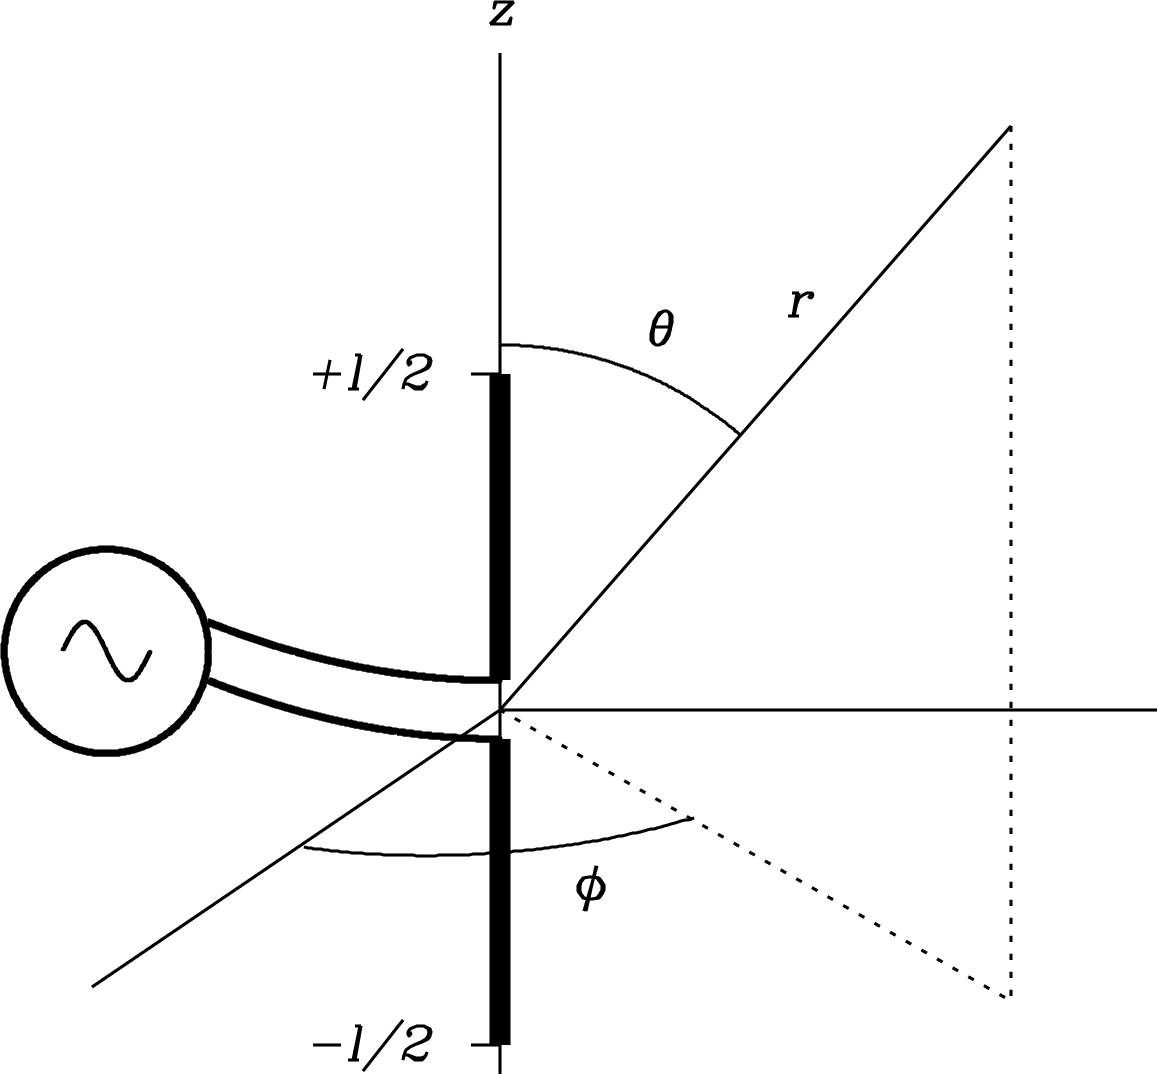
\includegraphics[width=0.5\textwidth]{short-dipole}
  \bicaption{%
    用于分析短偶极天线辐射的坐标系统
  }{%
    The coordinate system used to describe the radiation from a
    short dipole.
    \\来源/Credit:
    \citeay{condon2016}, \S\,3.1.1
  }
  \label{fig:short-dipole}
\end{figure}

首先考虑一个加速度为 $\dot{v}$ 的电荷 $q$,在距离 $r$ 处产生的切向
(即与 $r$ 的方向垂直)电场强度为
(详见 \citeay{condon2016}, \S\,2.7):
\begin{equation}
  \label{eq:q-efield}
  E_{\perp} = \frac{q \dot{v} \sin\theta}{r \acs{speed-light}^2} ,
\end{equation}
其中
\acs{speed-light} 是\acl{speed-light},
$\theta$ 为 $r$ 与 $v$ 之间的夹角。
天线的每一小段 $\D{z}$ 均会贡献一定的电场强度 $\D{E_{\perp}}$,
由于 $l \ll \lambda$,因此产生的总电场强度为:
\begin{equation}
  \label{eq:dipole-efield1}
  E_{\perp} = \int_{-l/2}^{l/2}
    \frac{\dot{v} \sin\theta}{r \acs{speed-light}^2} \,\diff{q}{z}\D{z} .
\end{equation}
对于远场情形 ($r \gg l$),$1/r$ 可视为常数而提出积分号。
考虑一个正弦形式的驱动电流:
\begin{equation}
  \label{eq:dipole-current}
  I = I_0 \,\Ce^{-\Ci \omega t} ,
\end{equation}
其中 $I_0$ 为电流峰值,
于是 $\dot{v} = -\Ci \omega v$。
导线中的电流可表示为:
\begin{equation}
  \label{eq:wire-current}
  I \equiv \diff{q}{t} = \diff{q}{z} \diff{z}{t} = \diff{q}{z} v ,
\end{equation}
代入\autoref{eq:dipole-efield1},可得
\begin{align}
  \label{eq:dipole-efield2}
  E_{\perp}
    & = -\frac{\Ci\omega \sin\theta}{r \acs{speed-light}^2}
      \int_{-l/2}^{l/2} \diff{q}{z} v \,\D{z} \\
    & = -\frac{\Ci\omega \sin\theta}{r \acs{speed-light}^2}
      \int_{-l/2}^{l/2} I\,\D{z} .
\end{align}
从天线的中点到两端,电流近似线性地减小至 0,即导线中的电流分布为:
\begin{equation}
  \label{eq:dipole-current-dist}
  I(z) \approx I_0 \,\Ce^{-\Ci\omega t}
    \left[ 1 - \frac{|z|}{l/2} \right] .
\end{equation}
最终可得天线在 $r$ 处产生的切向电场强度为:
\begin{align}
  E_{\perp}
    & \approx -\frac{\Ci\omega \sin\theta}{r \acs{speed-light}^2}
      \frac{I_0 l}{2} \Ce^{-\Ci\omega t} \\
    & = -\frac{\Ci\Cpi \sin\theta}{r \acs{speed-light}}
      \frac{I_0 l}{\lambda} \Ce^{-\Ci\omega t} .
    \label{eq:dipole-efield}
\end{align}
\autoref{fig:dipole-radiation} 显示了一个无限短偶极天线(即 Hertz 偶极子)
的瞬时电场强度分布图。

\begin{figure}[htp]
  \centering
  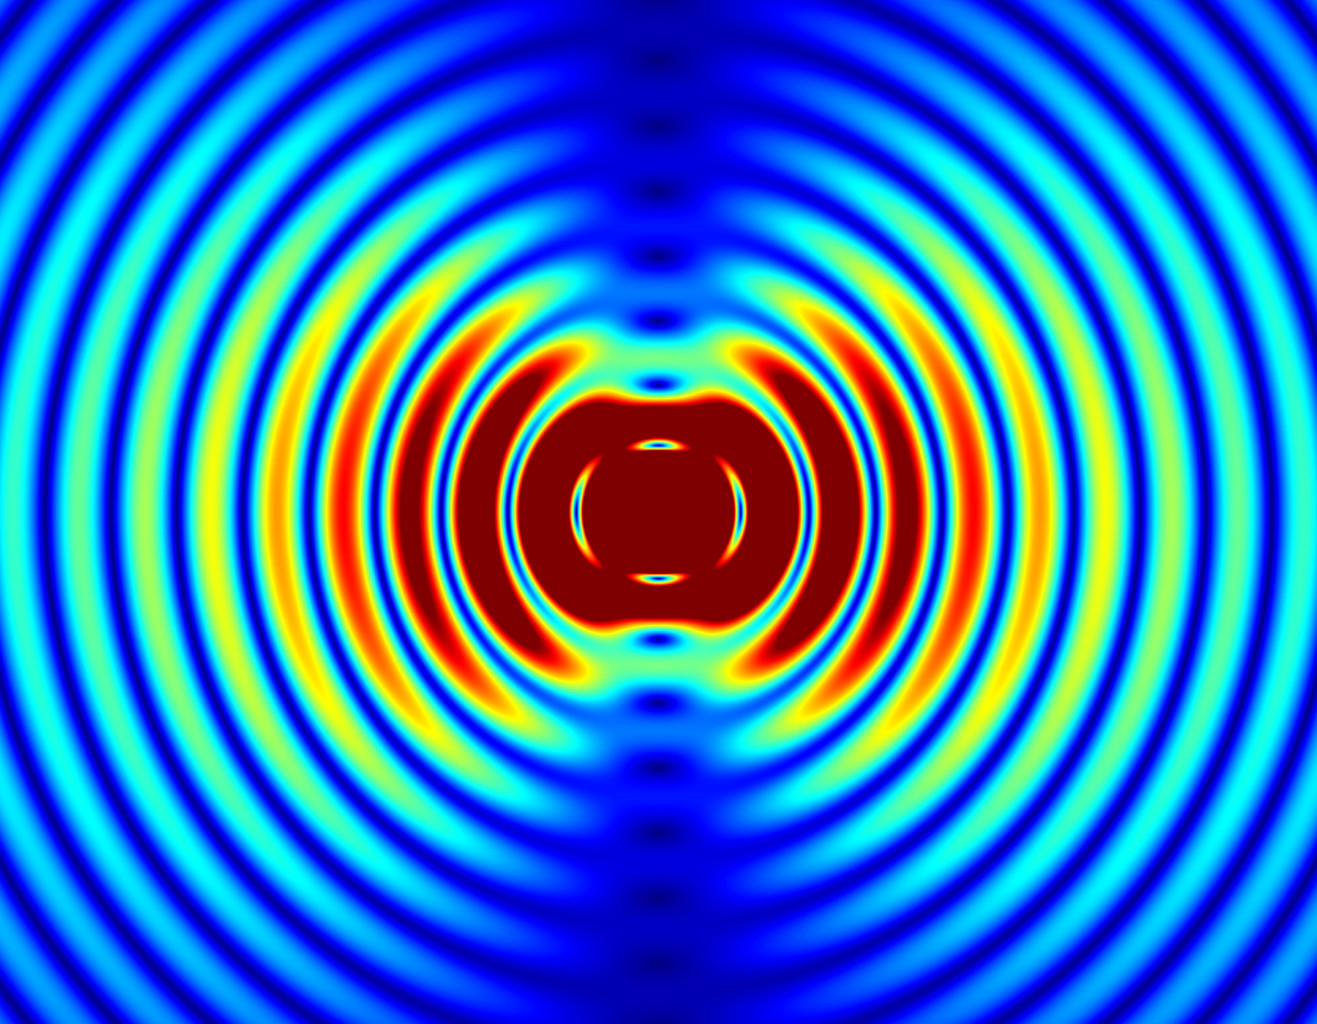
\includegraphics[width=0.6\textwidth]{hertzian-dipole-radiation}
  \bicaption{%
    Hertz 偶极子的瞬时电场强度分布图
  }{%
    The instantaneous electric field intensity distribution of
    a Hertzian dipole.
    \\来源/Credit:
    nageljr, \url{https://www.deviantart.com/nageljr/art/The-Hertzian-Dipole-Antenna-542377463}, (2019-03-18), \ac{cc} BY
  }
  \label{fig:dipole-radiation}
\end{figure}

%---------------------------------------------------------------------
\subsection{功率方向图和增益}

\acf{pp} $P(\theta,\phi)$ 是指一个天线的辐射功率的角向分布。
对于短偶极天线,由\autoref{eq:dipole-efield} 可得对时间平均的
Poynting 流量(即单位面积流过的功率)为:
\begin{equation}
  \label{eq:poynting-flux}
  \langle S \rangle
    = \frac{\acs{speed-light}}{4\Cpi} \langle E_{\perp}^2 \rangle
    = \frac{\Cpi}{8\,\acs{speed-light}}
      \left( \frac{I_0 l}{\lambda} \right)^2 \frac{\sin^2\theta}{r^2} .
\end{equation}
于是该天线的\ac{pp} $P(\theta,\phi)$ 为:
\begin{equation}
  P(\theta,\phi) = \langle S \rangle.
\end{equation}
在实际情况中,一般使用归一化的\ac{pp},即:
\begin{align}
  \label{eq:power-pattern}
  P_n(\theta,\phi)
    & \equiv P(\theta,\phi) / P_{\R{max}} \\
    & = \sin^2\theta .
\end{align}
对于更一般的天线,其\ac{pp} $P(\theta,\phi)$
将与两个空间方位角 $(\theta, \phi)$ 均相关。

\acf{gain} $G(\theta,\phi)$ 定义为天线在方向 $(\theta, \phi)$
的辐射功率 $P(\theta,\phi)$ 与一个总辐射功率相等但各向辐射同性的天线的辐射功率
$\bar{P}$ 之比,即:
\begin{equation}
  \label{eq:gain}
  G(\theta,\phi) = \frac{P(\theta,\phi)}{\bar{P}}
    = \frac{4\Cpi P(\theta,\phi)}{\int P(\theta,\phi) \,\D{\Omega}} .
\end{equation}
可见,天线的\ac{gain}与其\ac{pp}只相差一个常数。
对于一个理想的天线,全天平均的增益为:
\begin{equation}
  \label{eq:gain-avg}
  \langle G \rangle
    \equiv \frac{1}{4\Cpi} \int G(\theta,\phi) \,\D{\Omega}
    = 1 .
\end{equation}
在实际应用中,\ac{gain} $G$ 通常使用 [\si{\decibel}] 为单位:
\begin{equation}
    G_{\si{\decibel}} \equiv 10 \log_{10} G .
\end{equation}

%---------------------------------------------------------------------
\subsection{主瓣及其\acl*{hpbw}}

天线的\ac{pp} $P(\theta,\phi)$ 通常会在某个方向范围内具有
比在其他方向明显更大的值,
这个方向范围便称为天线的\acf{mainlobe},
其余方向的辐射瓣则称为\acf{sidelobe},如\autoref{fig:lobes} 所示。
主瓣的立体角 $\Omega_{\R{MB}}$ 定义为:
\begin{equation}
  \label{eq:omega-mb}
  \Omega_{\R{MB}} = \int_{\R{MB}} P_n(\theta,\phi) \,\D{\Omega} ,
\end{equation}
其中 $P_n(\theta,\phi)$ 为归一化的\ac{pp} [\autoref{eq:power-pattern}]。
主瓣的角度范围一般由\acf{hpbw}描述,定义为 $P(\theta,\phi)$
下降至最大值的一半时主瓣的两点之间的角距离(\autoref{fig:lobes})。
若天线的辐射越具有\ac{directivity},则天线的\ac{gain} $G$ 越大,
主瓣的立体角 $\Omega_{\R{MB}}$ 越小,\ac{hpbw} 也越小。

\begin{figure}[htp]
  \centering
  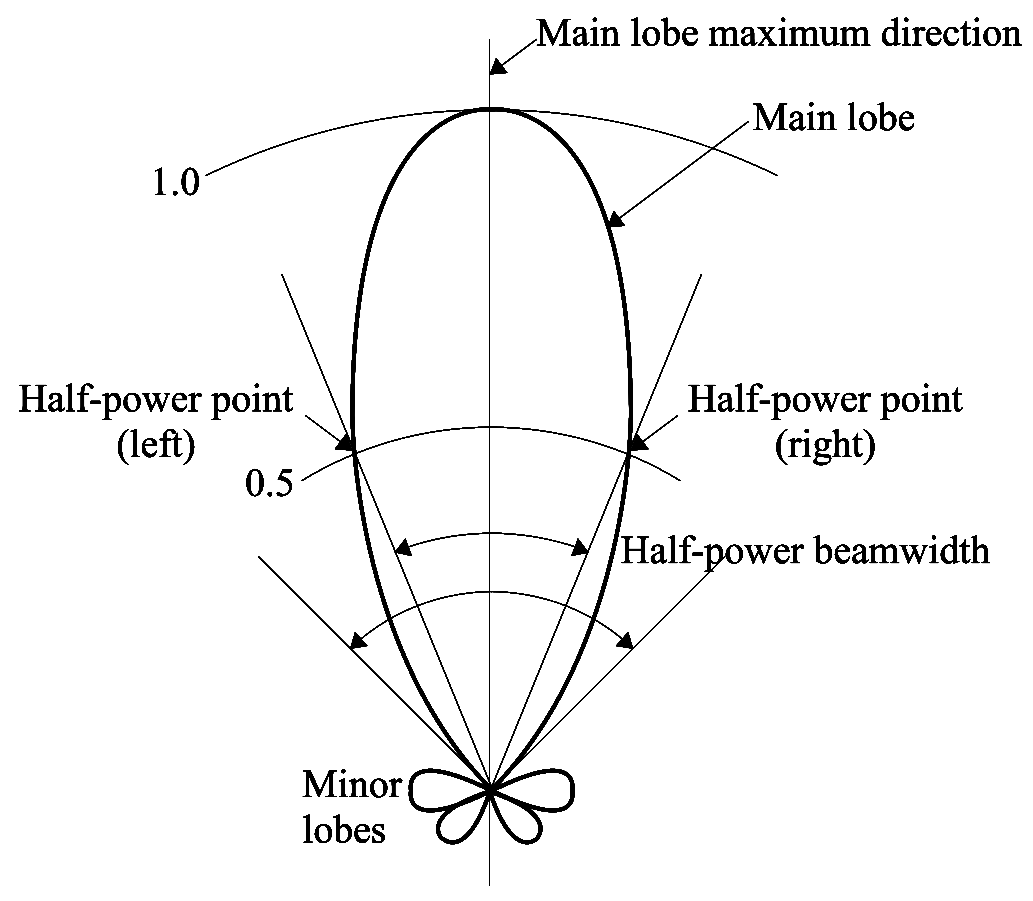
\includegraphics[width=0.6\textwidth]{antenna-lobes}
  \bicaption{%
    天线主瓣及其 HPBW 的示意图
  }{%
    Diagram of an antenna's main lobe and its HPBW.
    \\来源/Credit:
    \citeay{zuniga2009}
  }
  \label{fig:lobes}
\end{figure}

%---------------------------------------------------------------------
\subsection{有效接收面积}

在测量一个流量密度为 $S_{\nu}$ 的无偏振源时,
若天线输出的谱功率为 $P_{\nu}$,
则该天线的\acl{area-eff} (effective collecting area) \ac{area-eff}
定义为:
\begin{equation}
  \label{eq:area-eff}
  \ac{area-eff} \equiv \frac{2 P_{\nu}}{S_{\nu}} ,
\end{equation}
式中的因子 \enquote{2} 是因为单个天线只能响应一个偏振方向。

\begin{figure}[htp]
  \centering
  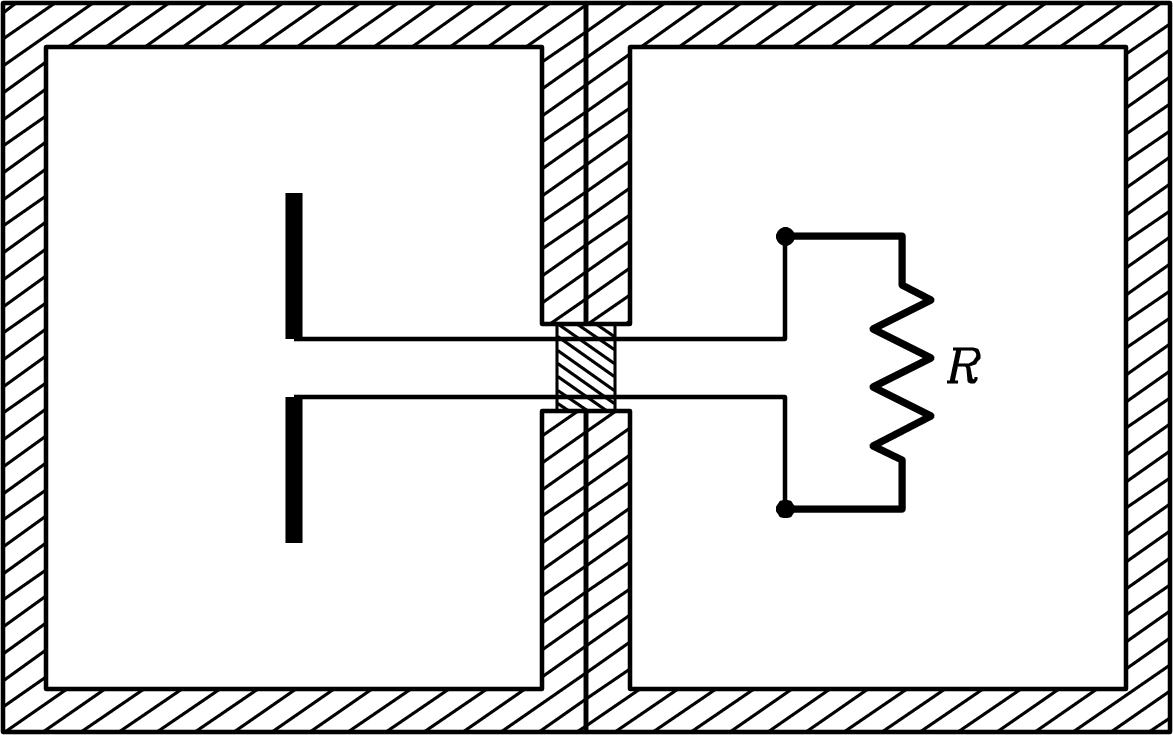
\includegraphics[width=0.5\textwidth]{average-area-thought-exp}
  \bicaption{%
    计算天线平均接收面积 $\langle \ac*{area-eff} \rangle$ 的思想实验
  }{%
    A thought experiment to calculate the average collection area
    $\langle \ac*{area-eff} \rangle$ of an antenna.
    \\来源/Credit:
    \citeay{condon2016}, \S\,3.1.4
  }
  \label{fig:area-avg-exp}
\end{figure}

天线的平均接收面积定义为:
\begin{equation}
  \label{eq:area-avg1}
  \langle \ac{area-eff} \rangle
    \equiv \frac{1}{4\Cpi} \int \ac{area-eff}(\theta,\phi) \,\D{\Omega} .
\end{equation}
为计算该面积,可借助这样一个思想实验:
一个理想的天线和一个理想的电阻,分别置于两个温度均为 $T$ 的空腔中并且达到热平衡;
天线和电阻之间使用导线相连,两个空腔之间设有一个特殊的阀门,能够阻挡电磁波,
但允许频率范围为 $[\nu, \,\nu+\D{\nu}]$ 的电流通过导线,
如\autoref{fig:area-avg-exp} 所示。
因为整个系统处于热平衡状态,所以导线中没有净能量流动,
否则其中一个空腔将升温、另一个则冷却,违背热力学第二定律。
因此,天线接收各个方向的无偏振黑体辐射 $B_{\nu}(T)$ 所产生的\ac{spec-power}为:
\begin{equation}
  P_{\nu,a} =
    \frac{1}{2} \int \ac{area-eff}(\theta,\phi) B_{\nu}(T) \,\D{\Omega} ,
\end{equation}
而且该\ac{spec-power}必须等于电阻的热噪声的\ac{spec-power} $P_{\nu,r}$。
代入\autoref{eq:nyquist} 和\autoref{eq:planck},可得
\begin{equation}
  \acs{kb}T =
    \frac{2\,\acs{kb}T}{2\lambda^2}
      \int \ac{area-eff}(\theta,\phi) \,\D{\Omega} ,
\end{equation}
其中 $\lambda = \ac{speed-light} / \nu$ 为辐射的波长,
于是天线的平均接收面积 $\langle \ac{area-eff} \rangle$ 为:
\begin{equation}
  \label{eq:area-avg}
  \langle \ac{area-eff} \rangle = \frac{\lambda^2}{4\Cpi} .
\end{equation}
由此可知,不同形状、大小的理想天线均具有相同的平均接收面积。
由\ac{reciprocity-theorem}可知,同一个天线的发射\ac{pp}与接收\ac{pp}相同,即:
\begin{equation}
  G(\theta,\phi) \propto A_e(\theta,\phi) .
\end{equation}
结合\autoref{eq:area-avg} 和\autoref{eq:gain-avg}
可得天线在某个方向的\acl{area-eff}为:
\begin{equation}
  \ac{area-eff}(\theta,\phi) = \frac{\lambda^2 G(\theta,\phi)}{4\Cpi} .
\end{equation}
若天线的\acl{area-eff} $\ac{area-eff}(\theta,\phi)$ 越大,
则天线在此方向的\ac{gain} $G(\theta,\phi)$ 也越大,
于是天线的\ac{directivity}越强,对其他方向的灵敏度越低。

%---------------------------------------------------------------------
\subsection{天线温度}

一个被置于温度为 $T$ 的黑体辐射环境中的天线,
输出的噪声将与温度为 $T$ 的电阻所产生的热噪声 [\autoref{eq:nyquist-approx}]
相同(即具有相同的频谱),该电阻被称为天线的匹配电阻。
若天线的输出谱功率为 $P_{\nu}$,则其匹配电阻的温度为
$T_r = P_{\nu} / \acs{kb}$,
于是定义\acl{T-antenna} (antenna temperature) 为其匹配电阻的温度,即:
\begin{equation}
  \label{eq:t-ant}
  \acs{T-antenna} \equiv T_r = \frac{P_{\nu}}{\acs{kb}} .
\end{equation}
\acl{T-antenna} \ac{T-antenna} 与天线的物理温度没有必然联系,
仅作为天线测量值的一个方便表示。
这个概念被广泛使用的原因主要有:
\begin{itemize}
  \item $\acs{T-antenna} = \SI{1}{\kelvin}$ 对应的谱功率为
    $P_{\nu} = \SI{1.38e-23}{\watt\per\hertz}$,
    是一个实用的小量,便于表示实际测量结果;
  \item 天线系统通常使用不同温度的电阻(称为负载)来进行校准,
    因此\acl{T-antenna}能够自然地表示校准结果;
  \item 接收机的噪声也使用 [\si{\kelvin}] 为单位,
    因此采用\acl{T-antenna}来描述信号强度能够简化信号和噪声的比较。
\end{itemize}

设天线的有效接收面积为 \ac{area-eff} [\autoref{eq:area-eff}],
则一个流量密度为 $S_{\nu}$ 的无偏振辐射源将使天线的温度 \acs{T-antenna} 上升:
\begin{equation}
  \label{eq:dt-source}
  \Delta\acs{T-antenna} = \frac{\ac{area-eff} S_{\nu}}{2\,\acs{kb}} .
\end{equation}


%=====================================================================
\section{射电干涉测量的基本原理}
\label{sec:interferometry}

根据衍射原理,望远镜的角分辨率约为 $\theta \sim \lambda / D$,
其中 $\lambda$ 为信号的波长(对应于观测频率),$D$ 为望远镜的口径。
射电信号的波长(约从亚毫米至数十米)远远大于光学波段的信号,
为了实现足够好的角分辨率,必须建造巨型的望远镜,
比如 \SI{100}{\meter} 口径的 \ac{gbt}、
\SI{305}{\meter} 口径的 Arecibo、
\SI{500}{\meter} 口径的 \ac{fast}。
然而在数百 \si{\MHz} 的低频射电波段,望远镜的口径需达到惊人的 \SI{10}{\km} 左右
才能在 \SI{100}{\MHz} 实现约 \SI{1}{\arcminute} 的角分辨率,
这对于单口径望远镜而言显然是不现实的。
因此,低频射电观测通常使用\ac{interferometry}技术,
通过联合一系列小望远镜开展相干测量并综合,获得高分辨率图像。

%---------------------------------------------------------------------
\subsection{二元单色干涉仪}

\begin{figure}[htp]
  \centering
  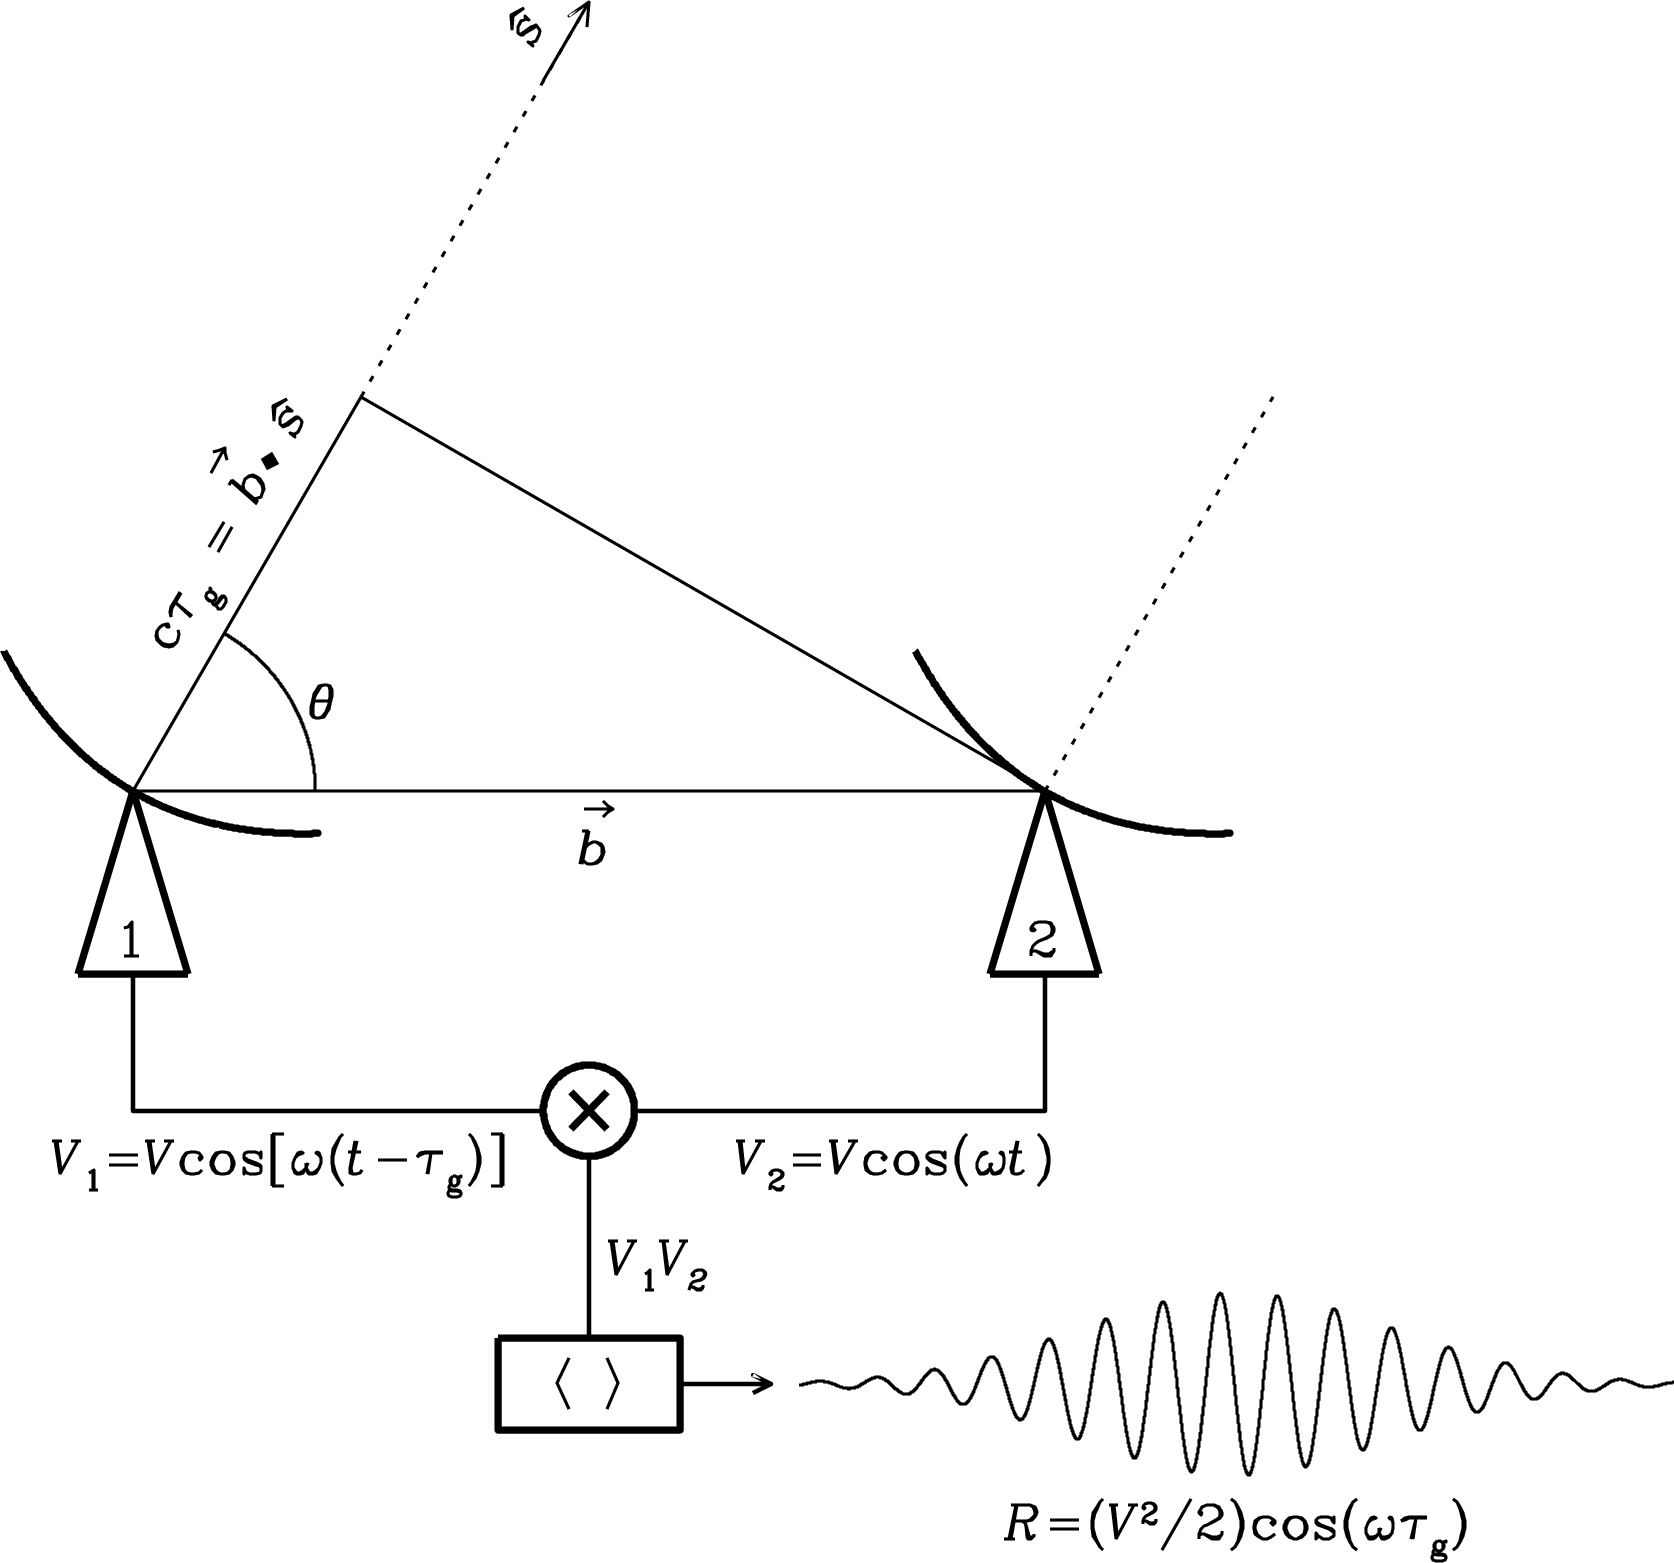
\includegraphics[width=0.7\textwidth]{interferometer}
  \bicaption[二元单色干涉仪的构成示意图]{%
    二元单色干涉仪的构成示意图。
    两个相同的天线相距 \ac*{v-baseline} 放置并指向位于 \ac*{v-direction} 方向的辐射源,
    接收的信号被放大后,再经过\acs*{correlator}的相乘 ($\times$)
    和时间平均 ($\langle\;\rangle$),得到输出响应 $R$。
  }{%
    The components of a two-element quasi-monochromatic interferometer
    observing in a very narrow radio frequency band centered at
    $\nu = \omega / (2\Cpi)$.
    The two identical antennas are separated by the baseline vector
    \ac*{v-baseline} and point to the source in direction \ac*{v-direction}.
    The signals received by the antennas are amplified,
    multiplied ($\times$), and time averaged ($\langle\;\rangle$)
    by the correlator to yield the output response $R$.
    \\来源/Credit:
    \citeay{condon2016}, \S\,3.7.1
  }
  \label{fig:interferometer}
\end{figure}

考虑一个最简单的二元单色干涉仪(如\autoref{fig:interferometer} 所示),
由两个相同的天线和\ac{correlator}构成,只测量频率为 $\nu$ 的单色信号。
由于辐射源非常遥远,其信号到达干涉仪时为平面波(忽略电离层扰动等影响)。
同一个波面被两个天线接收的时刻之间存在一定的差异,
即为\acl{delay-geo} (geometric delay) \ac{delay-geo}:
\begin{equation}
  \acs{delay-geo} =
    \frac{\ac{v-baseline} \cdot \ac{v-direction}}{\acs{speed-light}} ,
\end{equation}
其中 \acs{speed-light} 是\acl{speed-light},
\ac{v-baseline} 为两天线之间的\acl{v-baseline}(由天线 1 指向天线 2),
\ac{v-direction} 为辐射源的\acl{v-direction}。
两个天线接收信号后输出的电压响应分别为:
\begin{equation}
  \left\{
    \begin{aligned}
      V_1(t) &= V \cos [\omega (t - \acs{delay-geo})] , \\
      V_2(t) &= V \cos (\omega t) ,
    \end{aligned}
  \right.
\end{equation}
其中 $\omega = 2\Cpi\nu$ 为角频率。
\ac{correlator}然后将两个天线的响应相乘:
\begin{align}
  V_1(t) V_2(t)
    &= V^2 \cos [\omega (t - \acs{delay-geo})] \cos (\omega t) \\
    &= \frac{1}{2} V^2 \left[ \cos (2\omega t - \omega \acs{delay-geo})
      + \cos (\omega \acs{delay-geo}) \right] ,
\end{align}
接着再进行时间平均:
\begin{equation}
  \label{eq:resp-corr}
  R = \langle V_1(t) V_2(t) \rangle
    = \frac{1}{2} V^2 \cos (\omega \acs{delay-geo}) .
\end{equation}
由于天线响应 $V_1$ 和 $V_2$ 正比于辐射源的亮度和天线的\ac{gain}
[参见\autoref{eq:gain}],
因此\ac{correlator}的响应 $R$ 正比于辐射源的流量密度 $S$
和 $\sqrt{A_1 A_2}$,其中 $A_1$ 和 $A_2$ 为两个天线的有效接收面积
[参见\autoref{eq:area-avg}]。

当辐射源的方向 \ac{v-direction} 随地球的自转而改变时,
\acl{delay-geo} \acs{delay-geo} 也随之变化,
于是\ac{correlator}的输出 $R$ 出现正弦形式的振荡,
被称为干涉仪的响应\acf{fringe},
其相位为:
\begin{equation}
  \phi = \omega \acs{delay-geo}
    = 2\Cpi \left( \frac{b \cos\theta}{\lambda} \right) ,
\end{equation}
其中 $\theta$ 为\acl{v-direction} \ac{v-direction}
和\acl{v-baseline} \ac{v-baseline} 之间的夹角。
根据
\begin{equation}
  \diff{\phi}{\theta}
    = 2\Cpi \left( \frac{b \sin\theta}{\lambda} \right) ,
\end{equation}
可知单个\ac{fringe}的宽度 \acs{bw-synthesized} 为:
\begin{equation}
  \label{eq:bw-synthesized}
  \acs{bw-synthesized} = \frac{\lambda}{b \sin\theta} ,
\end{equation}
此参数称为干涉仪的\acl{bw-synthesized} (synthesized beamwidth),
描述了干涉仪的角分辨能力。

天线的\ac{pp}描述了天线响应随方向的变化情况,也被称为干涉仪的\acf{beam-primary},
将对输出 $R$ 产生调制,亦如\autoref{fig:interferometer} 所示,
其中\ac{correlator}的响应\ac{fringe}的\ac{envelope}示意了\ac{beam-primary}的衰减情况。

对于一个表面亮度分布为 $\acs{I-nu}(\ac{v-direction})$ 的\ac{src-extended},
由于不同位置产生的辐射互不相干,因此可以被当作一系列独立的点源处理,
于是上述二元单色干涉仪观测这个\ac{src-extended}的输出响应为:
\begin{align}
  R_c & = \int \acs{I-nu}(\ac{v-direction})
      \cos \left( \omega \ac{v-baseline} \cdot \ac{v-direction} /
        \acs{speed-light} \right)
      \,\D{\Omega}  \\
    & = \int \acs{I-nu}(\ac{v-direction}) \cos \left(
        2\Cpi\, \ac{v-baseline} \cdot \ac{v-direction} / \lambda \right)
      \,\D{\Omega} ,
    \label{eq:resp-cos}
\end{align}
其中下标 \enquote{$c$} 表示 \enquote{cosine} \ac{correlator}的输出,
以区分下文将要介绍的 \enquote{sine} \ac{correlator}。

任意一个亮度分布 $I$ 可分解为奇对称成分 $I_{\R{odd}}$
与偶对称成分 $I_{\R{even}}$ 之和,
但是\autoref{eq:resp-cos} 描述的 cosine \ac{correlator}只能测量其中的
偶对称成分 $I_{\R{even}}$,因为:
\begin{align}
  R_c & = \int \left[ I_{\R{odd}}(\ac{v-direction}) +
        I_{\R{even}}(\ac{v-direction}) \right]
      \cos \left( 2\Cpi\, \ac{v-baseline} \cdot \ac{v-direction} /
        \lambda \right)
      \,\D{\Omega}  \\
    & = \int I_{\R{even}}(\ac{v-direction}) \cos \left(
        2\Cpi\, \ac{v-baseline} \cdot \ac{v-direction} / \lambda \right)
      \,\D{\Omega} .
\end{align}
为了能够测量另一个奇对称成分 $I_{\R{odd}}$,
则需要一个 \enquote{sine} \ac{correlator},
可通过对其中一个天线的输出增加 $\Cpi/2$ 的相位延迟来实现,于是有:
\begin{align}
  R_s & = \int \left[ I_{\R{odd}}(\ac{v-direction}) +
        I_{\R{even}}(\ac{v-direction}) \right]
      \sin \left( 2\Cpi\, \ac{v-baseline} \cdot \ac{v-direction} /
        \lambda \right)
      \,\D{\Omega}  \\
    & = \int I_{\R{odd}}(\ac{v-direction}) \sin \left(
        2\Cpi\, \ac{v-baseline} \cdot \ac{v-direction} / \lambda \right)
      \,\D{\Omega} .
\end{align}
一对 cosine 和 sine \ac{correlator}的组合称为\ac{c-correlator},
其输出称为\acl{Vis} (complex visibility),简称\ac{vis}:
\begin{align}
  \acs{Vis}
    & \equiv R_c - \Ci\, R_s  \\
    & = \int \ac{I-nu}(\ac{v-direction}) \exp
      (-2\Cpi\Ci\, \ac{v-baseline} \cdot \ac{v-direction} / \lambda)
      \,\D{\Omega} .
    \label{eq:vis}
\end{align}

%---------------------------------------------------------------------
\subsection{有限带宽和平均时间的影响}

将上述二元单色干涉仪推广至有限带宽信号的测量。
考虑一个中心频率为 $\nu_c$ 且宽度为 $\Delta\nu$ 的窄频带 ($\Delta\nu \gg \nu_c$),
可认为辐射源的亮度和天线的响应在此频带内保持不变,
于是可得干涉仪测量的\ac{vis} [\autoref{eq:vis}] 为:
\begin{align}
  \acs{Vis}
    & = \int \left[ \frac{1}{\Delta\nu}
        \int_{\nu_c-\Delta\nu/2}^{\nu_c+\Delta\nu/2}
        I(\ac{v-direction}, \nu) \exp (-2\Cpi\Ci\, \nu\acs{delay-geo})
      \right] \,\D{\Omega} \\
    & \approx \int \ac{I-nu}(\ac{v-direction})
      \sinc_{\Cpi} (\Delta\nu\,\acs{delay-geo})
      \exp (-2\Cpi\Ci\, \nu_c\acs{delay-geo}) \,\D{\Omega},
  \label{eq:vis-bw}
\end{align}
其中归一化 $\sinc_{\Cpi}$ 函数的定义如下:
\begin{equation}
  \label{eq:sinc}
  \sinc_{\Cpi}(x) =
    \begin{dcases*}
      \frac{\sin(\Cpi x)}{\Cpi x}, \quad & if $x \neq 0$, \\
      1, \quad & if $x = 0$.
    \end{dcases*}
\end{equation}
因此对于带宽为 $\Delta\nu$ 的非单色信号,
干涉仪测得的\ac{fringe}幅度减弱至原来的
$\sinc_{\Cpi}(\Delta\nu\,\acs{delay-geo})$ 倍。
为了尽可能地减小这种信号衰减,可以给\enquote{前导}天线
(即先接收到信号的天线)的输出信号增加\acl{delay-comp}
(compensating delay) \ac{delay-comp},
使其满足 $|\acs{delay-comp} - \acs{delay-geo}| \ll (\Delta\nu)^{-1}$,
于是两个天线的输出响应到达\ac{correlator}时具有同步的相位
(如\autoref{fig:interferometer-tau0} 所示)。
满足 $\acs{delay-comp} = \acs{delay-geo}$ 的方向 $\ac{v-direction}_0$
称为\acf{delay-center}或\acf{phase-refpos}。

\begin{figure}[htp]
  \centering
  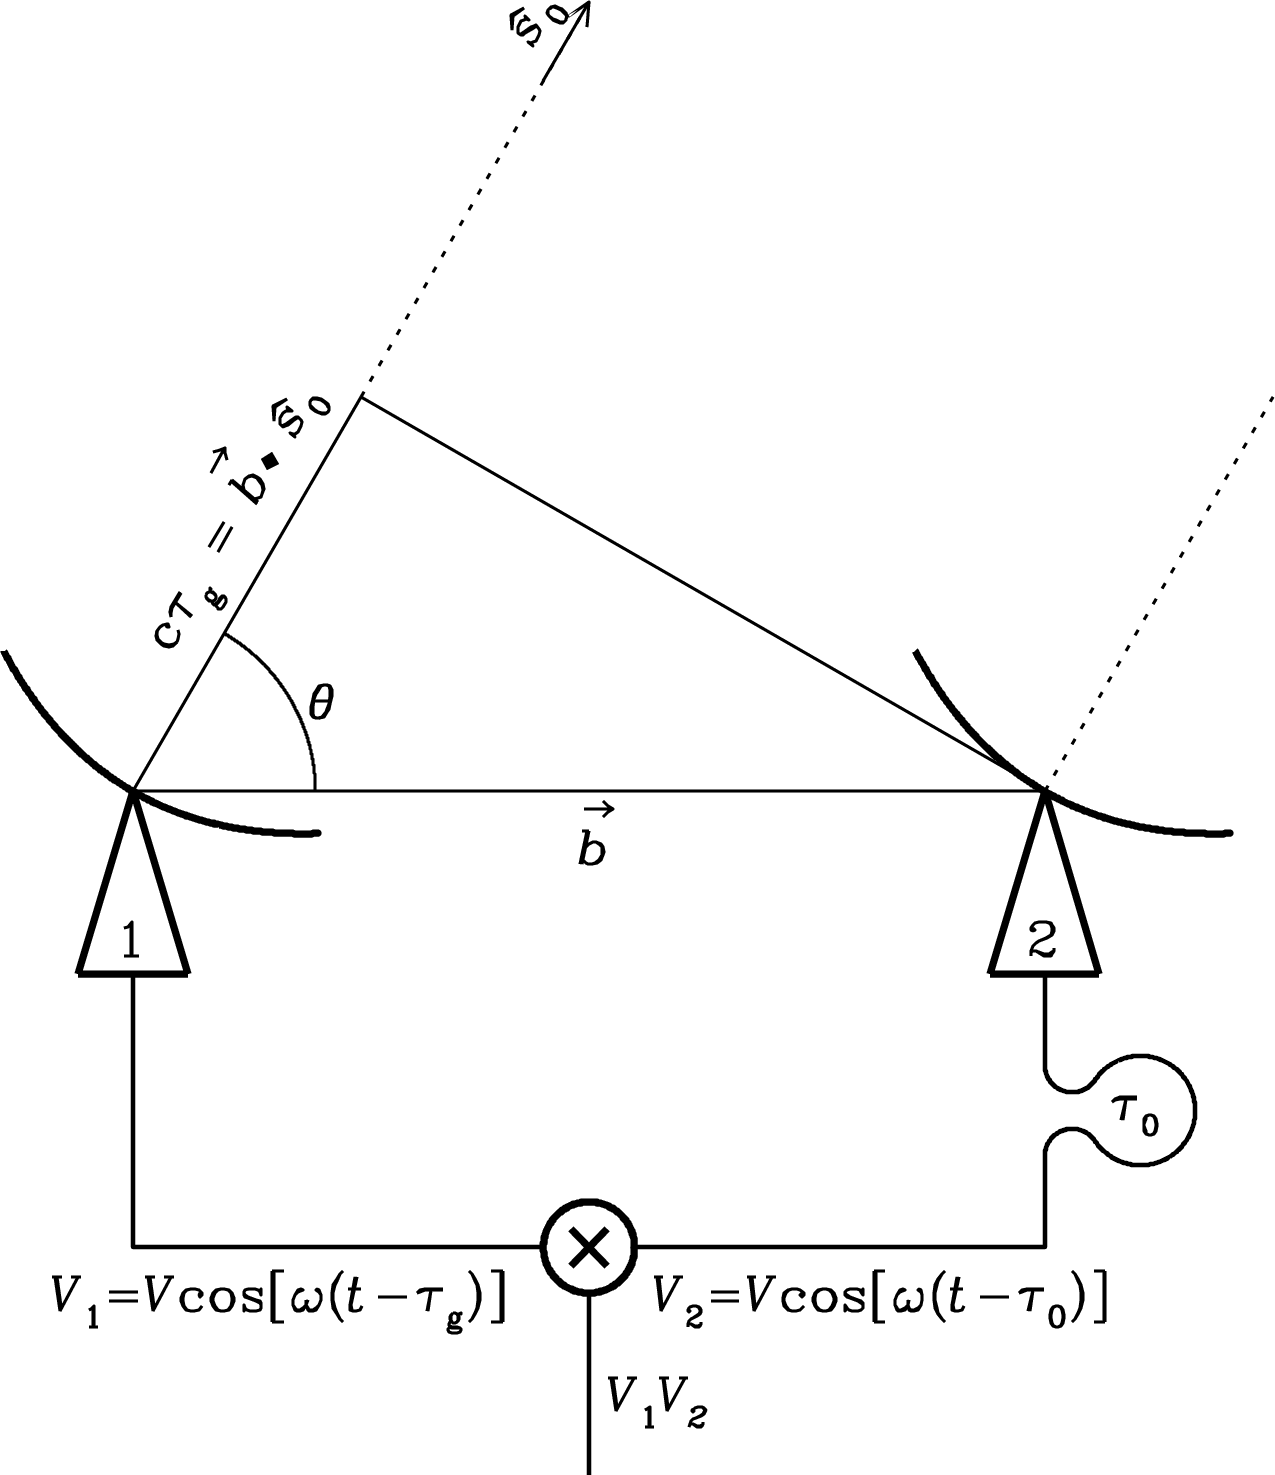
\includegraphics[width=0.6\textwidth]{interferometer-tau0}
  \bicaption[通过\acl*{delay-comp} \acs*{delay-comp} 来减小带宽效应的影响]{%
    通过给前导天线(对应于图中的天线 2)增加\acl*{delay-comp}
    $\acs*{delay-comp} \approx \acs*{delay-geo}$,
    使两个天线的输出信号的相位在相关运算时保持同步,
    从而最小化带宽效应的影响。
  }{%
    By introducing the compensating delay
    $\acs*{delay-comp} \approx \acs*{delay-geo}$ in the signal path of the
    leading antenna (i.e., the antenna 2), the phases of the two signals are
    almost in sync when they reach the correlator, hence minimizing the
    attenuation to the measured fringes caused by the finite bandwidth
    effect.
    \\来源/Credit:
    \citeay{condon2016}, \S\,3.7.3
  }
  \label{fig:interferometer-tau0}
\end{figure}

因为\acl{delay-geo} \acs{delay-geo} 会随方向 $\ac{v-direction}$ 而变化,
所以\acl{delay-comp} \acs{delay-comp} 只对特定方向 $\ac{v-direction}_0$
(即\ac{delay-center})是恰好准确的。
偏离\ac{delay-center}的角度 $\Delta\theta$ 越大,
\acl{delay-comp} \acs{delay-comp} 的修正效果就越差,
带宽效应产生的影响也就越严重。
这个效应被称为\acf{bw-smear},限制了有效的视场大小。
为了满足:
\begin{equation}
  \Delta\nu \Delta\acs{delay-geo}
    \approx \Delta\nu \diff{\acs{delay-geo}}{\theta} \Delta\theta
    = \frac{b \sin\theta}{\acs{speed-light}} \Delta\nu \Delta\theta
    \ll 1 ,
\end{equation}
则要求视场半径满足:
\begin{equation}
  \Delta\theta \ll \frac{\nu \acs{bw-synthesized}}{\Delta\nu} .
\end{equation}
解决\ac{bw-smear}的一个方法是将一个宽频带划分为一系列足够窄(约几十 \si{\kHz})
的频率\ac{channel},然后对每个\ac{channel}的信号独立地进行相关运算得到\ac{vis}。

类似地,如果\ac{correlator}的\ac{t-avg} $\Delta t$ 过长,
则辐射源的位置 \ac{v-direction} 会因地球自转而发生显著改变
(可与 \acs{bw-synthesized} 相比拟),
导致\acl{delay-comp} \acs{delay-comp} 的修正效果变差。
这个效应被称为\acf{t-smear}。
一个距离\ac{delay-center} $\Delta\theta$ 的目标的移动速度为
$v = \omega_e \Delta\theta$,其中 $\omega_e$ 为地球自转的角速度。
为了最小化\ac{t-smear}的影响,\ac{correlator}的\ac{t-avg} $\Delta t$ 需满足:
\begin{equation}
  v \Delta t = \omega_e \Delta\theta \Delta t \ll \theta_s ,
\end{equation}
即:
\begin{equation}
  \label{eq:correlator-avgtime}
  \Delta t \ll \frac{\theta_s}{\omega_e \Delta\theta} .
\end{equation}

%---------------------------------------------------------------------
\subsection{干涉成像原理}

\begin{figure}[htp]
  \centering
  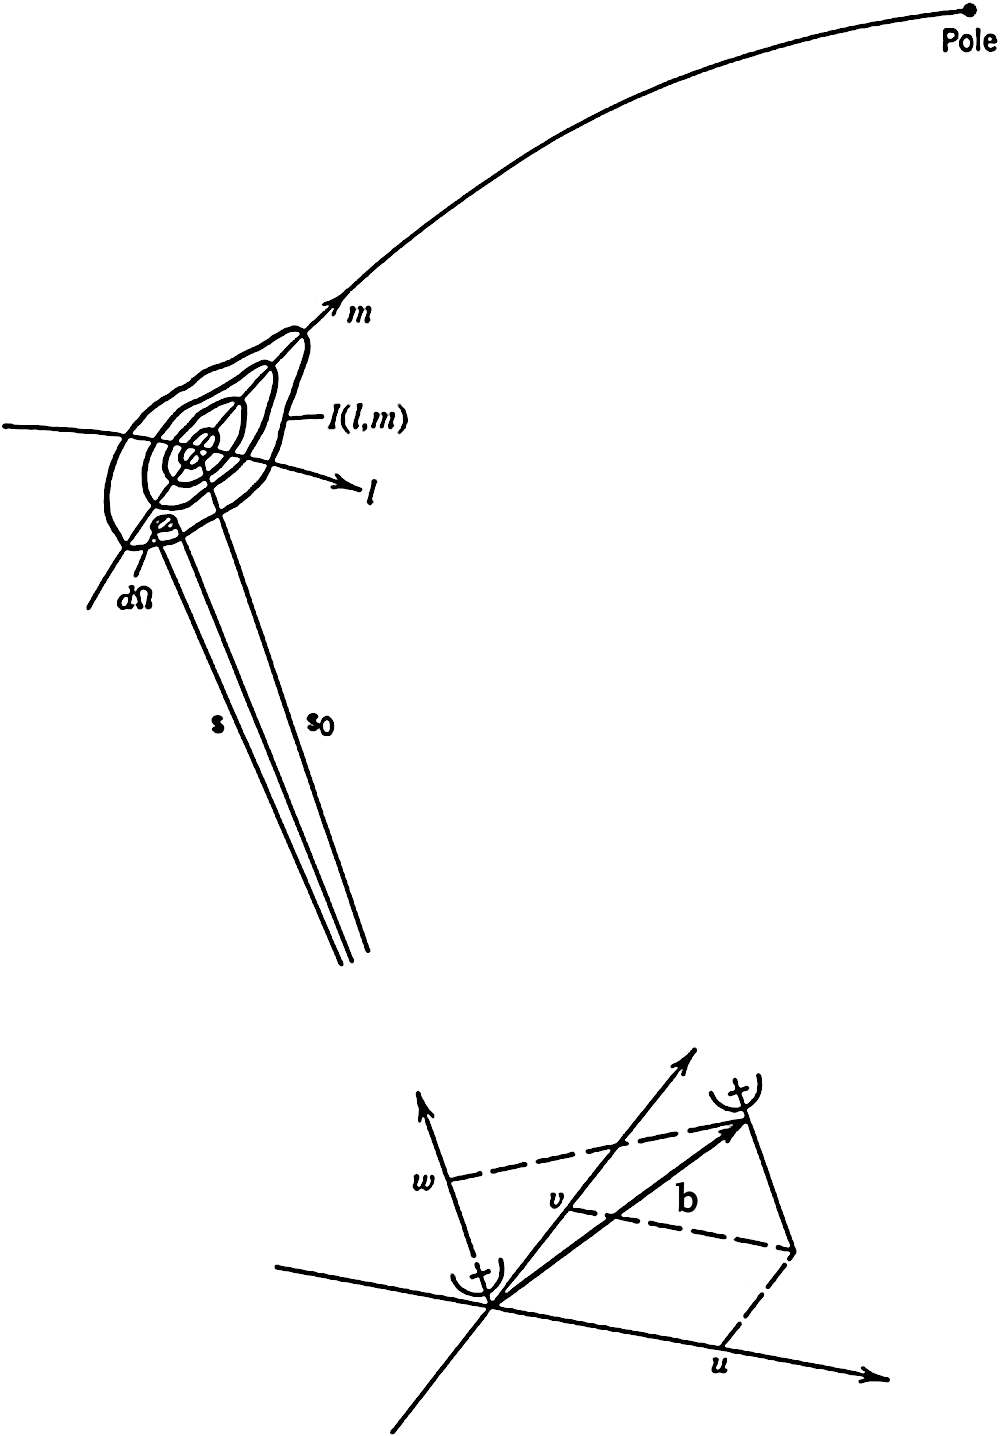
\includegraphics[width=0.7\textwidth]{interferometer-coordsys}
  \bicaption[干涉仪成像中常用的 $(u,v,w)$ 直角坐标系]{%
    干涉仪成像中常用的 $(u,v,w)$ 直角坐标系,
    其中 $w$ 轴指向参考方向 $\ac*{v-direction}_0$(通常为目标的中心),
    $u$ 轴向东,$v$ 轴向北。
    \acl*{v-baseline}可表示为 $\ac*{v-baseline} = (u,v,w) \lambda$,
    目标的亮度分布则用\acs*{dc}描述,
    即 $\ac*{I-nu}(\ac*{v-direction}) = \ac*{I-nu}(l,m)$,
    其中 $l, m$ 分别为\acl*{v-direction} \ac*{v-direction}
    对 $u, v$ 轴的投影长度。
  }{%
    The $(u,v,w)$ Cartesian coordinate system for interferometers,
    in which the $w$-axis points in the reference direction
    $\ac*{v-direction}_0$ (usually toward the source center), and
    the $u$- and $v$-axes point east and north, respectively.
    A baseline vector is represented as
    $\ac*{v-baseline} = (u,v,w) \lambda$,
    and the source brightness distribution is described as
    $\ac*{I-nu}(\ac*{v-direction}) = \ac*{I-nu}(l,m)$,
    where $l, m$ are direction cosines,
    i.e., the projected lengths of the direction vector \ac*{v-direction}
    against the $u$- and $v$-axes, respectively.
    \\来源/Credit:
    \citeay{thompson2017}, \S\,3.1
  }
  \label{fig:interferometer-coordsys}
\end{figure}

为了能够实际地运用\autoref{eq:vis} 从观测的\ac{vis}数据获得辐射源的亮度分布,
需要定义一个合适的坐标系。
如\autoref{fig:interferometer-coordsys} 所示的 $(u,v,w)$ 直角坐标系是最常用的,
其中 $w$ 轴指向参考方向 $\ac{v-direction}_0$(通常为目标的中心),
$u$ 轴向东,$v$ 轴向北。
于是\acl{v-baseline}为 $\ac{v-baseline} = (u,v,w) \lambda$,
\acl{v-direction}为 $\ac{v-direction} = \left( l, m, \sqrt{1-l^2-m^2} \right)$,
其中 $l$ 和 $m$ 分别为 \ac{v-direction} 对 $u$ 轴和 $v$ 轴的投影长度,即\ac{dc}。
再利用 $\D{\Omega} = \D{l}\,\D{m} \,\big/ \sqrt{1-l^2-m^2}$,
干涉仪测量的\ac{vis} [\autoref{eq:vis}] 便可表示为:
\begin{equation}
  \label{eq:vis-uvw}
  \acs{Vis}(u,v,w) = \iint \frac{\ac{I-nu}(l,m)}{\sqrt{1-l^2-m^2}}
    \exp \left[ -2\Cpi\Ci \left( ul+vm+w\sqrt{1-l^2-m^2} \right) \right]
    \,\D{l}\,\D{m} .
\end{equation}
注意,因为上式的相位因子存在额外项 \enquote{$w \sqrt{1-l^2-m^2}$},
所以这\emph{不是}二维 Fourier 变换。
但是在下述两种常见的特殊情况下,上式可变成二维 Fourier 变换,
从而可以通过逆 Fourier 变换从\ac{vis} \acs{Vis} 获得目标的亮度分布 $\ac{I-nu}(l,m)$。
\begin{itemize}
\item
\emph{所有\acl{v-baseline}共面:}
这里可以进一步分为两种情形:
(1) 干涉阵列的天线只沿东西方向分布,如 \ac{wsrt} \cite{hogbom1974wsrt},
尽管\acl{v-baseline}随地球自转而发生变化,
所有\acl{v-baseline}均落在同一个垂直于地球自转轴的平面内;
(2) 虽然干涉阵列的天线呈二维分布,如 \ac{miteor} \cite{zheng2014},
但是采用\ac{snapshot}观测模式,即每次观测或成像的\ac{t-int}足够短。
在这两种情况下,可以选取合适的坐标系原点使得 $w = 0$,
于是\autoref{eq:vis-uvw} 变成二维 Fourier 变换,
通过逆变换可得目标的亮度分布:
\begin{equation}
  \label{eq:vis-inv1}
  \frac{\ac{I-nu}(l,m)}{\sqrt{1-l^2-m^2}}
    = \iint \acs{Vis}(u,v, w \equiv 0)
      \exp [2\Cpi\Ci\, (ul+vm)] \,\D{u}\,\D{v} .
\end{equation}

%.......................................
\item
\emph{小视场成像:}
对于任何干涉阵列,如果只观测以参考方向 $\ac{v-direction}_0$
为中心的一个足够小的视场区域,则有:
\begin{equation}
  w \sqrt{1-l^2-m^2}
    \approx w \left[ 1 - \frac{l^2+m^2}{2} \right] .
\end{equation}
于是\autoref{eq:vis-uvw} 成为:
\begin{multline}
  \acs{Vis}(u,v,w) \approx \exp (-2\Cpi\Ci\,w) \\
    \times \iint\! \frac{\ac{I-nu}(l,m)}{\sqrt{1-l^2-m^2}}
    \exp [-2\Cpi\Ci\, (ul+vm) -\Ci\Cpi w(l^2+m^2)] \,\D{l}\,\D{m} .
\end{multline}
如果 $\big| \Cpi w(l^2+m^2) \big| \ll 1$,
即有 $\exp [-\Ci\Cpi w(l^2+m^2)] \approx 1$,
则上式变成二维 Fourier 变换,即:
\begin{align}
  \acs{Vis}(u,v)
    & \equiv \acs{Vis}(u,v,w) \exp (2\Cpi\Ci\,w)  \\
    & = \iint \frac{\ac{I-nu}(l,m)}{\sqrt{1-l^2-m^2}}
    \exp [-2\Cpi\Ci\, (ul+vm)] \,\D{l}\,\D{m} ,
  \label{eq:vis-uv}
\end{align}
然后通过逆 Fourier 变换,便得到目标的亮度分布:
\begin{equation}
  \label{eq:vis-inv2}
  \frac{\ac{I-nu}(l,m)}{\sqrt{1-l^2-m^2}}
    = \iint \acs{Vis}(u,v)
      \exp [2\Cpi\Ci\, (ul+vm)] \,\D{u}\,\D{v} .
\end{equation}

\end{itemize}

上述第一种情况要求\acl{v-baseline} \ac{v-baseline} 全部在同一平面内,
第二种情况要求\acl{v-direction} \ac{v-direction}
在天球上的对应点全部在同一平面内,即视场足够小。
从\autoref{eq:vis} 容易看出 \ac{v-baseline} 和 \ac{v-direction} 之间存在对称性,
因此这两种情况可理解为相同近似条件的不同表现形式 \cite{clark1999}。
如果无法满足以上两种情况(比如呈三维空间分布的干涉阵列的大视场成像),
则需要采用专门的成像方法 \cite{cornwell1992,sault2007},
例如 \ac{w-proj}法 \cite{cornwell2008}、
\ac{w-stack}法 \cite{humphreys2011}
(将在 \autoref{sec:obs-simu} 使用的 \texttt{WSClean} 成像软件实现了该方法
\cite{offringa2014,offringa2017})。

%---------------------------------------------------------------------
\subsection{\texorpdfstring{$uv$}{uv} 覆盖和脏图}
\label{sec:uv-coverage}

设二元干涉仪的\acl{v-baseline}为 $\ac{v-baseline} = (u,v,w)\lambda$,
干涉仪在每个时刻测量 $uv$ 平面内位于 $(u,v)$ 和 $(-u,-v)$ 的一对\ac{vis}数据点。
\ac{v-baseline} 的各个分量随地球自转而逐渐变化,
于是该基线在 \SI{24}{\hour} 内测量的\ac{vis}数据点在 $uv$ 平面内形成两个相互对称的椭圆。
一个包含 \ac{N-ant} 个天线的干涉阵列可形成
$\ac{N-ant}(\ac{N-ant}-1)/2$ 条基线,
每条基线都可以测量 $uv$ 平面内相应位置的\ac{vis},
于是显著地增加了 $uv$ 覆盖度,即 $uv$ 平面内被测量到的范围。
\autoref{fig:uv-coverages} 展示了不同天线数目、不同\ac{t-int}的 $uv$ 覆盖。

\begin{figure}[htp]
  \centering
  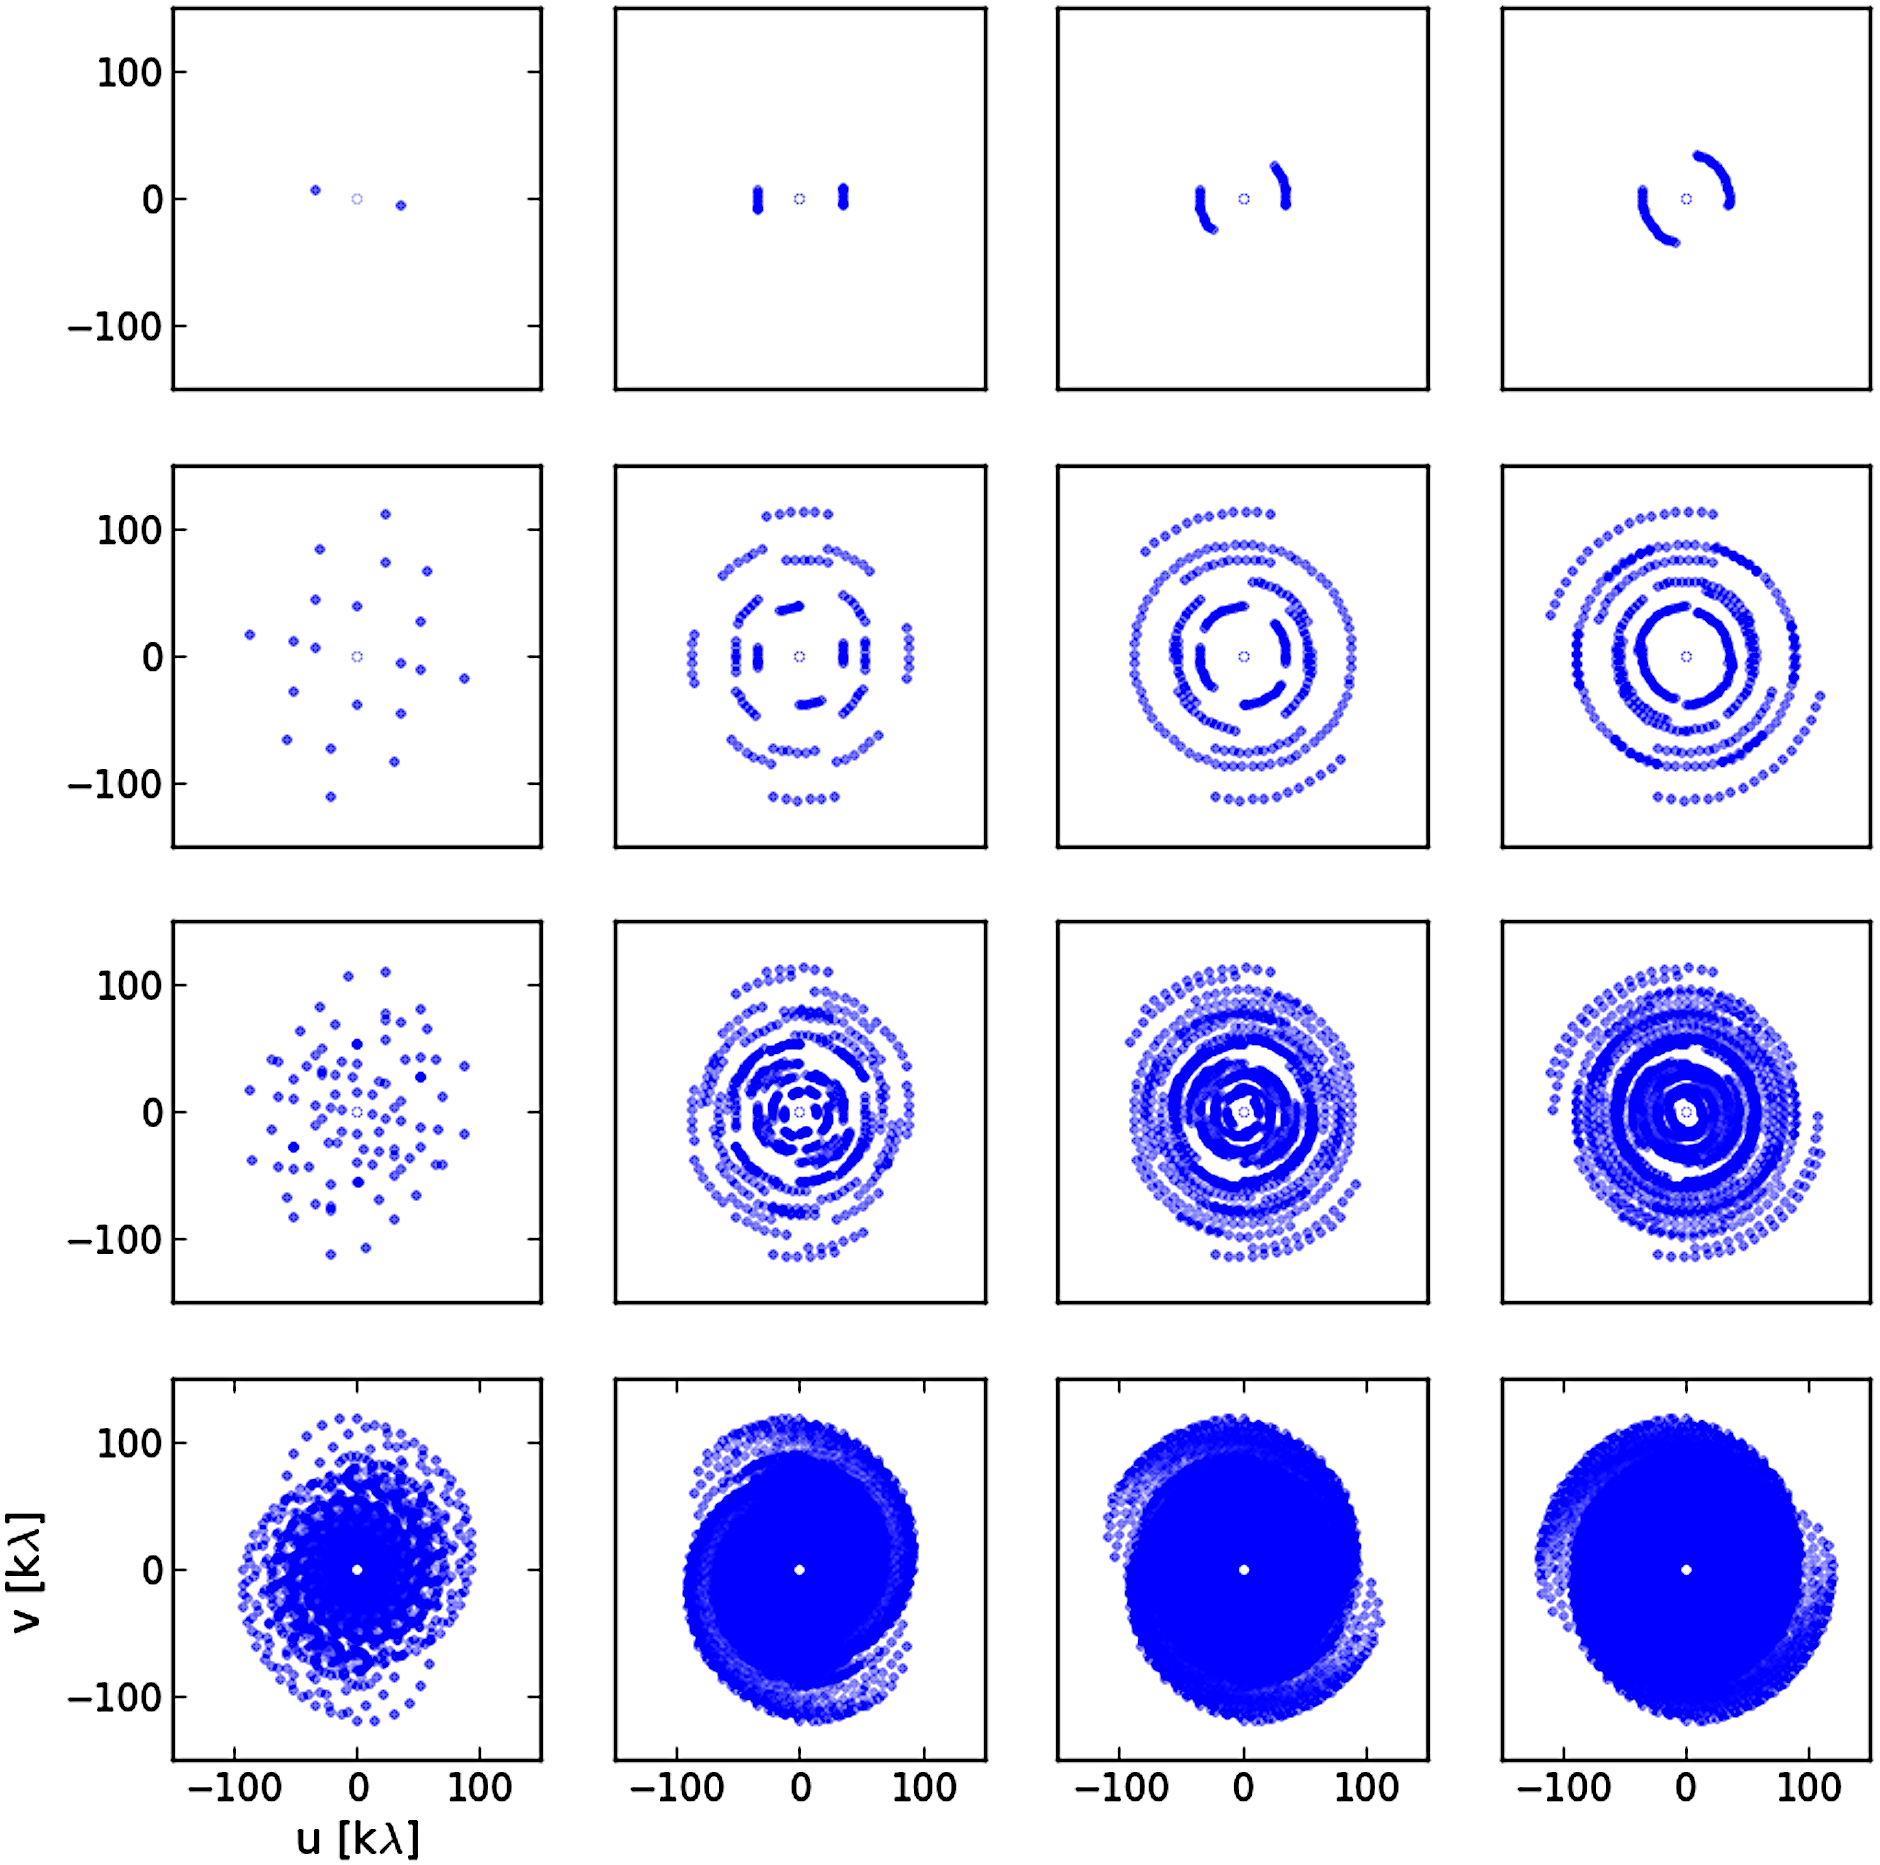
\includegraphics[width=\textwidth]{uv-coverages}
  \bicaption[不同天线数目、不同积分时间的 $uv$ 覆盖示例]{%
    不同天线数目、不同积分时间的 $uv$ 覆盖示例。
    \uline{从上往下}: 干涉阵列分别包含 2、5、10 和 50 个呈对数螺旋状分布的天线;
    \uline{从左到右}: \ac{t-int}分别为 \SI{10}{\second}、\SI{2}{\hour}、
    \SI{4}{\hour} 和 \SI{6}{\hour}。
  }{%
    Examples of $uv$ coverages.
    \uline{Top to bottom}: the interferometer includes 2, 5, 10, and 50
    antennas in a logarithmic spiral pattern, respectively;
    \uline{Left to right}: the integration time is \SI{10}{\second},
    \SI{2}{\hour}, \SI{4}{\hour}, and \SI{6}{\hour}, respectively.
    \\来源/Credit:
    \citeay{avison2013}
  }
  \label{fig:uv-coverages}
\end{figure}

因为干涉阵列的天线数目是有限的,基线的长度范围也是有限的,
所以在实际观测中 $uv$ 平面不可能被完全覆盖,
具体覆盖情况可由\acf{f-sampling}描述:
\begin{equation}
  \label{eq:sf}
  \acs{S-uv} = \sum_{k,t} \delta(u - u_{k,t}, v - v_{k,t}) ,
\end{equation}
其中 $u_{k,t}$ 和 $v_{k,t}$ 为时刻 $t$ 时基线 $\B{b}_k$ 在 $uv$ 平面内的分量。
于是,干涉阵列实际测量的\ac{vis}数据为:
\begin{equation}
  \label{eq:vis-measured}
  \acs{Vis}^{m}(u,v) = \acs{Vis}(u,v) \,\acs{S-uv} .
\end{equation}
由于无法获得目标亮度分布的全部信息,
根据\autoref{eq:vis-inv2} 对测量的\ac{vis}数据进行逆 Fourier 变换
仅能得到目标的\acf{map-dirty} $I_{\nu}^D(l,m)$:
\begin{equation}
  \label{eq:dirty-map}
  \frac{I_{\nu}^D(l,m)}{\sqrt{1-l^2-m^2}} = \iint
    \acs{Vis}(u,v) \acs{S-uv} \exp [2\Cpi\Ci\, (ul+vm)] \,\D{l}\,\D{m} .
\end{equation}
利用\ac{conv-theorem},可将上式表示为:
\begin{equation}
  I_{\nu}^D(l,m) = \ac{I-nu}(l,m) * B(l,m) ,
\end{equation}
其中 \enquote{$*$} 表示卷积算符,
$B(l, m)$ 是\ac{f-sampling} \acs{S-uv} 的 Fourier 变换:
\begin{equation}
  \label{eq:syn-beam}
  B(l,m) = \iint \acs{S-uv} \exp [2\Cpi\Ci\, (ul+vm)] \,\D{l}\,\D{m} ,
\end{equation}
称为\acf{beam-synthesized}或\acf{psf}。
\autoref{fig:imaging-relations} 展示了成像过程中的主要变换关系。
为了从\ac{map-dirty} $I_{\nu}^D(l,m)$ 尽可能地恢复目标的真实图像 $\ac{I-nu}(l,m)$,
则需要使用复杂的非线性\ac{deconv}方法,
比如 CLEAN 算法 \cite{hogbom1974,cornwell1999}
(详见后文 \autoref{sec:clean})、\ac{mem} \cite{narayan1986}。

\begin{figure}[htp]
  \centering
  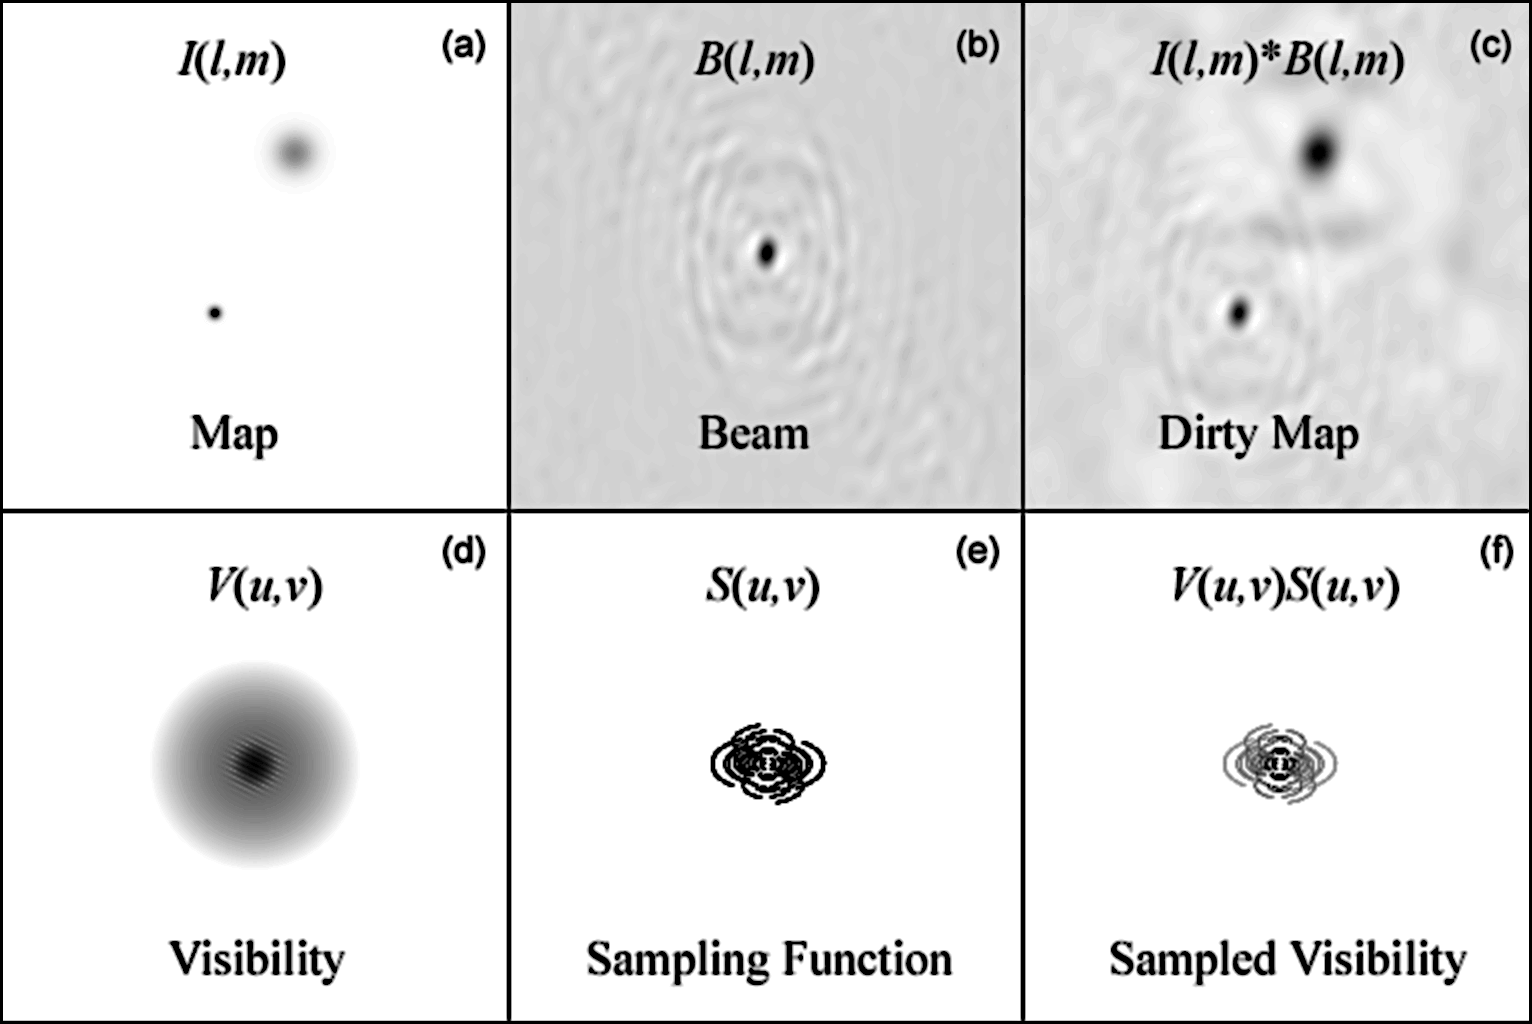
\includegraphics[width=\textwidth]{imaging-relations}
  \bicaption[干涉成像过程中的变换关系]{%
    干涉成像过程中的变换关系。
    \emph{(a)} 真实天图;
    \emph{(b)} \acs*{beam-synthesized};
    \emph{(c)} 脏图;
    \emph{(d)} 真实的\acs*{vis}数据;
    \emph{(e)} \acs*{f-sampling};
    \emph{(f)} 实际测量的\acs*{vis}数据。
    每列的两张图像互为 Fourier 变换。
  }{%
    The transform relations among the imaging process.
    \emph{(a)} True sky map;
    \emph{(b)} Synthesized beam;
    \emph{(c)} Dirty map;
    \emph{(d)} True visibility data;
    \emph{(e)} Sampling function;
    \emph{(f)} Actually measured visibility data.
    The two images in each column are the Fourier transform of each other.
    \\来源/Credit:
    Dale E. Gary, Radio Astronomy, Lecture 6,
    \url{https://web.njit.edu/~gary/728/Lecture6.html}, (2018-11-21)
    [反转了颜色]
  }
  \label{fig:imaging-relations}
\end{figure}

%---------------------------------------------------------------------
\subsection{栅格化和加权方法}

干涉成像过程涉及大量的 Fourier 变换,因此严重依赖于\ac{fft}算法,
该算法的计算复杂度为 $\mathcal{O}(N \log N)$,其中 $N$ 为数据点数目,
远远低于离散 Fourier 变换的计算复杂度 $\mathcal{O}(N^2)$,尤其当 $N$ 很大的时候。
\ac{fft} 算法要求数据分布在均匀的\ac{grid}上,
因此需要对观测的\ac{vis}数据 [\autoref{eq:vis-measured}] 进行\ac{gridding},即:
\begin{equation}
  \acs{Vis}^{G}(u,v)
    = \frac{1}{\Delta u \Delta v}
      \Sha\!\left( \frac{u}{\Delta u}, \frac{v}{\Delta v} \right)
      \acs{Vis}^{m}(u,v) ,
\end{equation}
其中
$\Sha()$ 为 Shah 函数(亦称 Dirac 梳状函数):
\begin{equation}
  \Sha(x, y) = \sum_{i,j=-\infty}^{\infty} \delta(x-i, y-j) ,
\end{equation}
$\Delta u$ 和 $\Delta v$ 为 $uv$ \ac{grid}的\ac{cell}大小。

干涉阵列能够测量的最小 $u_{\R{min}}$ 和 $v_{\R{min}}$
由其最短基线 $b_{\R{min}}$ 决定:
\begin{equation}
  u_{\R{min}} \approx v_{\R{min}} \approx b_{\R{min}}/\lambda .
\end{equation}
根据信号处理领域的\ac{sampling-theorem},
为了避免数据因\ac{gridding}而出现失真,\ac{grid}的\ac{cell}大小应满足:
\begin{equation}
  \Delta u \approx \Delta v
    \lesssim \frac{u_{\R{min}}}{2} \approx \frac{v_{\R{min}}}{2}
    \approx \frac{b_{\R{min}}}{2 \lambda} .
\end{equation}
另一方面,干涉阵列的最长基线 $b_{\R{max}}$ 决定了能够测量的
$u_{\R{max}}$ 和 $v_{\R{max}}$:
\begin{equation}
  u_{\R{max}} \approx v_{\R{max}} \approx b_{\R{max}}/\lambda .
\end{equation}
因此\ac{gridding}之后的 $uv$ 平面的每边\ac{cell}数目为:
\begin{equation}
  N_u \approx N_v \gtrsim \frac{2 b_{\R{max}}}{b_{\R{min}}} .
\end{equation}

干涉阵列的短基线主要测量目标辐射的大尺度分布情况(对应于 $u$、$v$ 较小的\ac{vis}数据),
长基线则主要探测目标辐射的小尺度结构(对应于 $u$、$v$ 较大的\ac{vis}数据)。
根据研究对象和目标的不同,需要从同一份观测数据处理得到不同性质的图像,
比如,研究点源形态时要求图像的空间分辨率高,探测展源时则要求图像的噪声水平低。
因此在成像过程中需要对\ac{vis}数据进行加权处理,即:
\begin{equation}
  \acs{Vis}^{w}(u,v) = \acs{Vis}^{G}(u,v) W(u,v) ,
\end{equation}
其中 $W(u,v)$ 为\ac{f-weighting}。
常用的加权方法有以下三种:
\begin{itemize}
  \item \emph{自然权重}:
    每个\ac{cell}的权重 $W_n(u_i, v_j)$ 为该\ac{cell}所包含的数据点个数
    $N(u_i, v_j)$。
    假定一个\ac{cell}内的数据服从正态分布,则该\ac{cell}的数据方差为:
    $\sigma^2(u_i, v_j) \simeq 1/N(u_i, v_j)$。
    因此,采用自然权重使每个\ac{cell}的权重反比于\ac{cell}的方差,即:
    \begin{equation}
      W_n(u_i, v_j) = N(u_i, v_j) \simeq \frac{1}{\sigma^2(u_i, v_j)} ,
    \end{equation}
    如此所得的图像具有最低的噪声水平,适合用于探测暗弱展源。
    因为 $uv$ 平面中心区域的覆盖通常远好于外围区域,
    所以自然权重会使短基线得到的权重大于长基线,
    因此图像的空间分辨率较差,并且旁瓣较明显。
  
  \item \emph{均匀权重}:
    每个\ac{cell}的权重 $W_u(u_i, v_j)$ 反比于该\ac{cell}所包含的数据点个数
    $N(u_i, v_j)$,即:
    \begin{equation}
      W_u(u_i, v_j) = \frac{1}{N(u_i, v_j)} .
    \end{equation}
    这种加权方法使长基线得到更大的权重,使 $uv$ 平面的覆盖更均匀,
    所以生成的图像的空间分辨率较好,旁瓣较弱,但是图像的噪声水平较高。
  
  \item \emph{Briggs 权重}:
    亦称稳健 (robust) 权重,是均匀权重和自然权重的折衷,
    通过调节稳健参数来控制两种加权方法的作用程度 \cite{briggs1995}。
    稳健参数的典型取值范围为 $[-1, 1]$;
    参数值越小,加权效果越接近均匀权重,参数值越大,则越接近自然权重。
    但是,取稳健参数为 $-1$ 或 $1$ 并不等效于使用均匀或自然权重。
\end{itemize}
\autoref{fig:imaging-weighting} 对比了上述三种加权方法的成像效果。

\begin{figure}[htp]
  \begin{minipage}{0.33\textwidth}
    \centering
    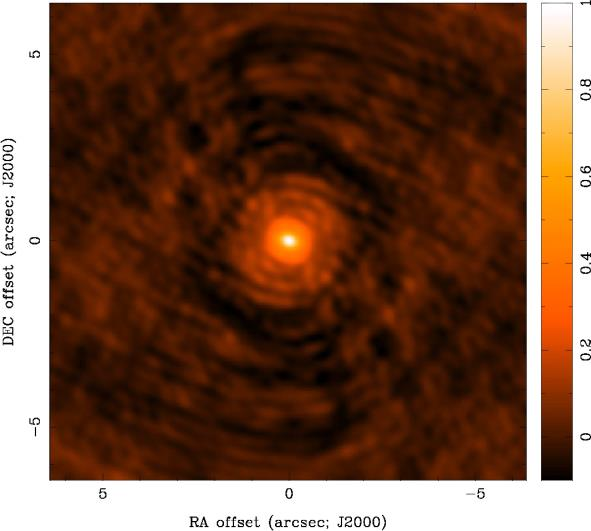
\includegraphics[width=\linewidth]{weighting-natural} \\
    (a) Natural
  \end{minipage}%
  \hfill%
  \begin{minipage}{0.33\textwidth}
    \centering
    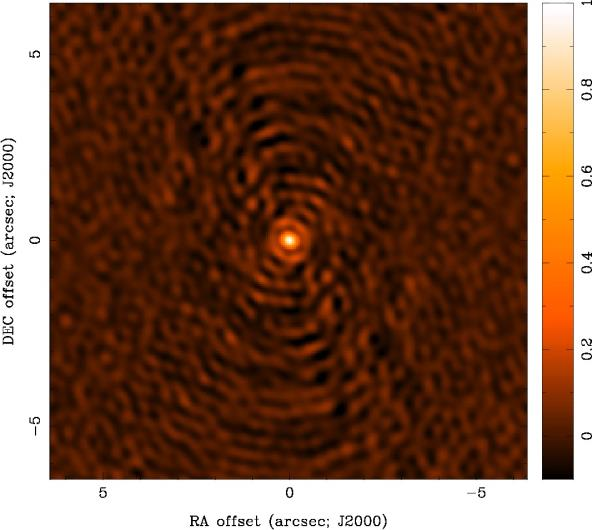
\includegraphics[width=\linewidth]{weighting-uniform} \\
    (b) Uniform
  \end{minipage}%
  \hfill%
  \begin{minipage}{0.33\textwidth}
    \centering
    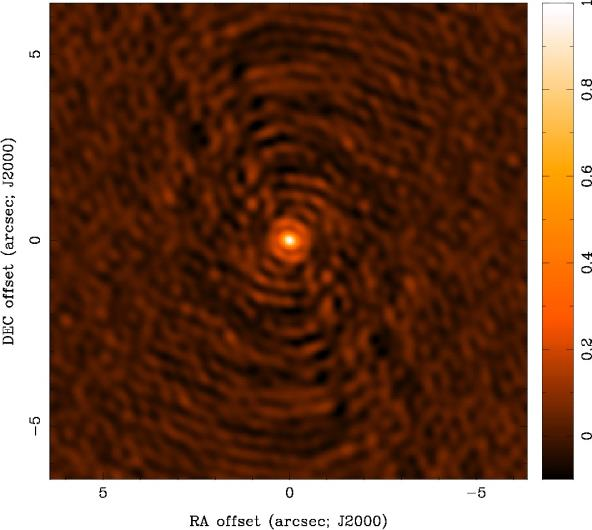
\includegraphics[width=\linewidth]{weighting-robust} \\
    (c) Briggs
  \end{minipage}
  \bicaption[自然权重、均匀权重和 Briggs 权重的成像效果对比]{%
    自然权重、均匀权重和 Briggs 权重的成像效果对比。
    \emph{(a)} 自然权重:
      空间分辨率为 \SI{0.59 x 0.50}{\arcsecond},噪声水平为 1.0\,Jy/beam;
    \emph{(b)} 均匀权重:
      空间分辨率为 \SI{0.35 x 0.30}{\arcsecond},噪声水平为 2.1\,Jy/beam;
    \emph{(c)} Briggs 权重(稳健参数为 0):
      空间分辨率为 \SI{0.40 x 0.34}{\arcsecond},噪声水平为 1.3\,Jy/beam。
  }{%
    A comparison of imaging results among different weighting methods.
    \emph{(a)} Natural weighting:
      the angular resolution is \SI{0.59 x 0.50}{\arcsecond}
      and the noise level is 1.0\,Jy/beam;
    \emph{(b)} Natural weighting:
      the angular resolution is \SI{0.35 x 0.30}{\arcsecond}
      and the noise level is 2.1\,Jy/beam;
    \emph{(c)} Natural weighting:
      the angular resolution is \SI{0.40 x 0.34}{\arcsecond}
      and the noise level is 1.3\,Jy/beam.
    \\来源/Credit:
    David J. Wilner, 2016, Imaging and Deconvolution,
    15th Synthesis Imaging Workshop,
    \url{https://science.nrao.edu/science/meetings/2016/15th-synthesis-imaging-workshop/}
  }
  \label{fig:imaging-weighting}
\end{figure}

%---------------------------------------------------------------------
\subsection{CLEAN 算法和洁图}
\label{sec:clean}

因为无法获得目标亮度分布的全部信息,即 $uv$ 平面覆盖不完备,
得到的\ac{map-dirty}存在非常明显的仪器旁瓣等干扰结构,与真实\ac{skymap}差异显著
(如\autoref{fig:imaging-relations} 和\autoref{fig:imaging-weighting} 所示),
不适合直接用于科学分析。
为了得到质量更佳的图像,一方面可以通过开展额外观测来改进 $uv$ 平面的覆盖度,
另一方面可以利用先验知识对 $uv$ 平面未被覆盖的区域进行插值,称为\ac{deconv}过程
\cite{cornwell1999}。

在射电天文学中,由 \citeauthor{hogbom1974} 在 \citeyear{hogbom1974}
提出的 CLEAN 算法 \cite{hogbom1974} 是使用最为广泛的\ac{deconv}算法。
CLEAN 算法假定目标源可以表示成一系列点源,具体内容如下:
\begin{itemize}
  \item \emph{输入}:
    \begin{itemize}
      \item \ac{map-dirty} $I^D$ [\autoref{eq:dirty-map}]
      \item \ac{beam-synthesized} $B$ [\autoref{eq:syn-beam}]
    \end{itemize}
  \item \emph{参数}:
    \begin{itemize}
      \item \ac{loop-gain} $g$:通常取 0.1
      \item 最大迭代次数 $n$
      \item CLEAN 阈值 $s$
    \end{itemize}
  \item \emph{初始化}:
    \begin{itemize}
      \item CLEAN 成分集合 $L$:空
      \item \ac{map-residual} $I^r$:等于\ac{map-dirty} $I^D$
    \end{itemize}
  \item \emph{迭代过程}:
    \begin{enumerate}
      \item 在\ac{map-residual} $I^r$ 中寻找绝对强度最大的点,
        得到该峰值点的位置 $p$ 和强度 $A$;
      \item 在峰值点 $p$,从 $I^r$ 减去 $g A B$,
        得到更新的\ac{map-residual},即:
        $I^r \gets I^r - g A B$;
      \item 将峰值点的信息($p$ 和 $A$)添加到集合 $L$;
      \item 判断是否满足下述停止条件,如果满足其中任意一个,则结束迭代并输出结果,
        否则跳转至第 1 步继续下一轮迭代。
        \begin{itemize}
          \item 当前迭代次数 $i > n$
          \item $I^r$ 的峰值点强度 $|A| < s$
        \end{itemize}
    \end{enumerate}
  \item \emph{输出}:
    \begin{enumerate}
      \item 使用椭圆高斯模型拟合\ac{beam-synthesized} $B$ 的主瓣,
        所得结果称为\ac{beam-clean} $B^C$;
      \item 从 CLEAN 成分集合 $L$ 生成\ac{map-model} $I^m$;
      \item 最后输出的\ac{map-clean} $I^C = I^m * B^C + I^r$,
        其中 $I^r$ 为迭代结束时的\ac{map-residual}。
    \end{enumerate}
\end{itemize}
\autoref{fig:imaging-clean} 展示了 CLEAN 过程中的各种图像。

\begin{figure}[htp]
  \centering
  \begin{minipage}{0.32\textwidth}
    \centering
    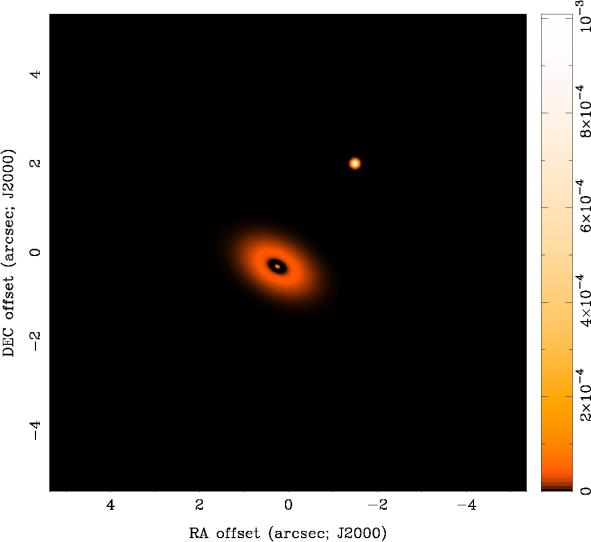
\includegraphics[width=\linewidth]{imaging-true} \\
    (a) True map
  \end{minipage}
  \begin{minipage}{0.32\textwidth}
    \centering
    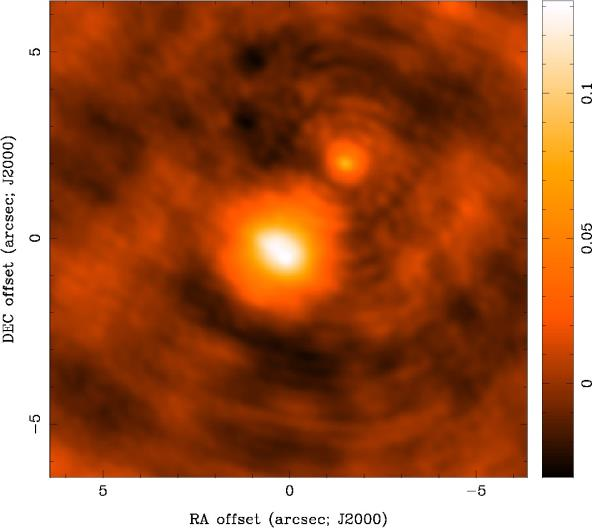
\includegraphics[width=\linewidth]{imaging-dirty} \\
    (b) Dirty map
  \end{minipage}
  \begin{minipage}{0.32\textwidth}
    \centering
    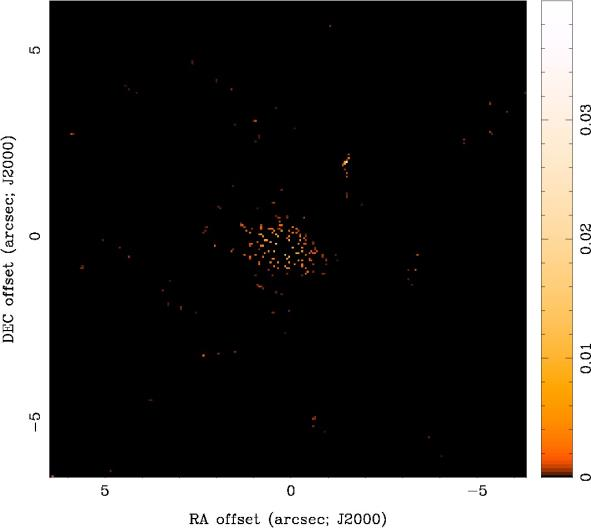
\includegraphics[width=\linewidth]{imaging-model} \\
    (c) Model map
  \end{minipage}%
  \\[0.5ex]
  \begin{minipage}{0.32\textwidth}
    \centering
    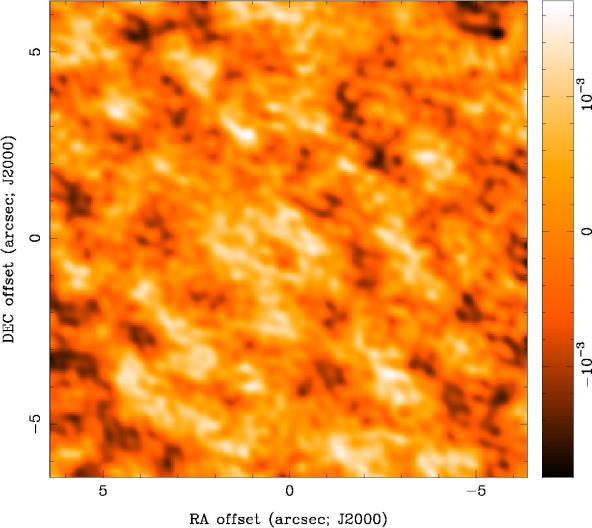
\includegraphics[width=\linewidth]{imaging-residual} \\
    (d) Residual map
  \end{minipage}
  \begin{minipage}{0.32\textwidth}
    \centering
    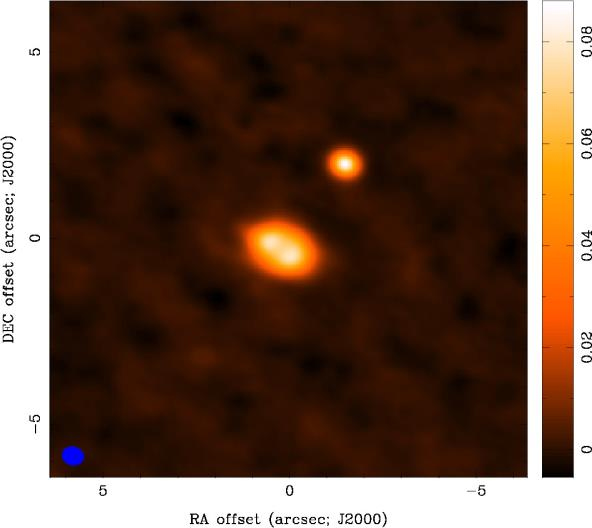
\includegraphics[width=\linewidth]{imaging-clean} \\
    (e) Clean map
  \end{minipage}
  \bicaption[从脏图得到洁图的 CLEAN 算法示例]{%
    从脏图得到洁图的 CLEAN 算法示例。
    \emph{(a)} 真实的天图 $I$;
    \emph{(b)} 脏图 $I^D$;
    \emph{(c)} CLEAN 得到的模型图 $I^m$,图中的点表示算法找到的 CLEAN 成分;
    \emph{(d)} CLEAN 迭代结束时的残差图 $I^r$;
    \emph{(e)} 洁图 $I^C$,图中左下角的蓝点表示洁波束 $B^C$ 的大小。
  }{%
    An illustration of the CLEAN algorithm that derives the clean map
    from the dirty map.
    \emph{(a)} True sky map $I$;
    \emph{(b)} Dirty map $I^D$;
    \emph{(c)} Model map $I^m$ created from all the found CLEAN compoments;
    \emph{(d)} Residual map $I^r$ when the CLEAN iteration process finished;
    \emph{(e)} Clean map $I^C$ with the blue blob in the bottom-left
    corner indicating the size of the clean beam $B^C$.
    \\来源/Credit:
    David J. Wilner, 2016, Imaging and Deconvolution,
    15th Synthesis Imaging Workshop,
    \url{https://science.nrao.edu/science/meetings/2016/15th-synthesis-imaging-workshop/}
  }
  \label{fig:imaging-clean}
\end{figure}

尽管 CLEAN 算法假定真实的辐射分布由一系列点源构成,
但是该算法处理展源的效果也相当好。
除了上面详细介绍的经典 Högbom 算法 \cite{hogbom1974},
CLEAN 算法还有多个变种,其中最重要的两种是 Clark 算法 \cite{clark1980}
和 Cotton--Schwab 算法 \cite{schwab1984}。

%---------------------------------------------------------------------
\subsection{点源灵敏度和亮度灵敏度}

天线的输出信号会因为自身的热噪声而存在一定的误差。
若天线的温度为 \ac{T-antenna} [参见\autoref{eq:t-ant}],
则每个时刻天线的测量值的\ac{rms}误差为
$\sigma_1 \approx \sqrt{2} \ac{T-antenna}$
(详见 \citeay{condon2016}, 附录 B.6)。
设信号的带宽为 $\Delta\nu$,根据\ac{sampling-theorem},
在\ac{t-int} $\tau$ 内应采样 $N \gtrsim 2 \Delta\nu \,\tau$ 个数据点,
于是天线的测量值误差减小为:
\begin{equation}
  \label{eq:radiometer}
  \sigma_{\tau}
    = \frac{\sqrt{2} \ac{T-antenna}}{\sqrt{N}}
    \approx \frac{\ac{T-antenna}}{\sqrt{\Delta\nu \,\tau}} .
\end{equation}
\ac{t-int}越长,测量值的误差就越小,观测所达到的灵敏度就越高。
然而在实际情况中,多种系统误差会限制灵敏度的提高,
比如天线和接收机的\ac{gain}变化、大气层辐射的不规则涨落、
未分辨背景源的\ac{confusion}、等等。

若一个无偏振点源的辐射使天线的温度 \ac{T-antenna} 升高了 $\Delta\ac{T-antenna}$,
则根据\autoref{eq:dt-source} 可测得该点源的流量密度为:
\begin{equation}
  S_{\nu} = \frac{2\,\ac{kb} \Delta\ac{T-antenna}}{\ac{area-eff}} ,
\end{equation}
相应的测量误差为:
\begin{align}
  \sigma_S
    & = \frac{2\,\ac{kb}}{\ac{area-eff}}
        \sigma(\ac{T-antenna} + \Delta\ac{T-antenna}) \\
    & \approx \frac{2\,\ac{kb}}{\ac{area-eff}} \sigma(\ac{T-antenna}) \\
    & = \frac{2\,\ac{kb} \ac{T-antenna}}{
      \ac{area-eff} \sqrt{\Delta\nu \,\tau}} ,
\end{align}
其中使用了\autoref{eq:radiometer},此即单天线的点源灵敏度。

对于由两个相同天线构成的二元干涉仪,其点源灵敏度为:
\begin{equation}
  \sigma_S
    = \frac{\sqrt{2}\,\ac{kb} \ac{T-antenna}}{
        \ac{area-eff} \sqrt{\Delta\nu \,\tau}} .
\end{equation}
由 \ac{N-ant} 个相同天线构成的干涉阵列可形成 $\ac{N-ant}(\ac{N-ant}-1)/2$
个独立的二元干涉仪,因此其点源灵敏度 $\sigma_S$ 为:
\begin{equation}
  \label{eq:sigma-ps}
  \sigma_S
    = \frac{2\,\ac{kb} \ac{T-antenna}}{
        \ac{area-eff} \sqrt{\ac{N-ant}(\ac{N-ant}-1) \Delta\nu \,\tau}} .
\end{equation}

如果观测一个\ac{src-extended},则需要考虑干涉仪的亮度灵敏度 $\sigma_b$,
可利用 Rayleigh--Jeans 近似 [\autoref{eq:rj-approx}] 由 $\sigma_S$ 导出:
\begin{equation}
  \label{eq:sigma-tb}
  \sigma_b = \frac{\lambda^2}{2\,\ac{kb}} \frac{\sigma_S}{\Omega_s} ,
\end{equation}
其中 $\Omega_s$ 是干涉阵列的\ac{beam-synthesized}的立体角。
相比单口径望远镜,干涉阵列的基线长、角分辨率高,
所以\ac{beam-synthesized}的立体角 $\Omega_s$ 非常小。
即使干涉阵列包含许多天线,但其亮度灵敏度 $\sigma_b$
与单口径望远镜相比并不具备优势。


%% EOF
